%-------------------------------------------------------------------------------
\section{Results}
\label{sec:result}
%-------------------------------------------------------------------------------

This section presents the results obtained from the individual channels, as well as their combination,
by following the statistical analysis discussed in Section~\ref{sec:stat_analysis}.

A binned likelihood fit under the signal-plus-background hypothesis is performed on the BDT discriminant distributions in the seven 
signal regions. The unconstrained parameter of the fit is the signal strength.
%and four independent parameters associated with the normalisation of the fake $\had$ background in each of the analysis regions. 
No significant pulls or constraints are obtained for the fitted nuisance parameters, resulting in a post-fit background prediction in each analysis region that is
very close to the pre-fit prediction, albeit with reduced uncertainties
%due to the anti-correlations among sources of systematic uncertainty
resulting from the fit.
%Figure~\ref{fig:Bonlyfit_data} shows a background only fit to the BDT discriminant distribution in the data.
Figures~\ref{fig:asimov_postfitbdtHu} and~\ref{fig:asimov_postfitbdtHc} show the BDT output distributions after the signal-plus-background fit to the 
data for the $tcH$ and $tuH$ searches, respectively.
%both pre- and post-fit to data, in the case of the $\Hc$ search.  
%A similar comparison for the leptonic channel is shown in Figure~\ref{fig:tthML_trexPrefit} and \ref{fig:tthML_trexPrefit_1}.
The observed and predicted yields after a background-only fit to the data are summarised in Table~\ref{tab:HtautauPostfitYieldsUnblind}.
%pre-fit and post-fit yields can be found in Appendix~\ref{sec:prepostfit_yields_Htautau_appendix}.
A slight excess of data events, with a significance of 2.3$\sigma$, is observed above the expected background. This is mainly in the high BDT-score region of the most sensitive channel, $t_{\ell}\thadhad$, as shown in Figures~\ref{fig:asimov_postfitbdtHu}(a) and~\ref{fig:asimov_postfitbdtHc}(a).
%Table~\ref{tab:limits_summary}.
The kinematic distributions for the observed excess in
the high BDT-score region were checked. Within the large statistical uncertainty, the observed distributions are compatible with the background shapes, but also with a small signal contribution. There is no indication that the excess is from a specific data period.
The background modelling in this signal region was also checked using the VR in which both $\thad$ candidates have the same charge.
%The BDT distribution in this VR is shown in Fig.##,
In this VR the signal contribution is negligble in the highest BDT bins and the background shape is well reproduced by the data.
%The fitted signal strength and its significance from individual channels and their combination are shown in Table~\ref{tab:limits_summary}.
%and found there are nothing unusual between data and expectation.
% \begin{figure}[H]
% \centering
% \begin{tabular}{@{}ccc@{}}
% %\includegraphics[width=0.33\textwidth]{\FCNCFigures/unblinded/tthML/tcH_reg1l2tau1bnj_os_postFit_BOnly.pdf}&
% %\includegraphics[width=0.33\textwidth]{\FCNCFigures/unblinded/tthML/tcH_reg1l1tau1b1j_ss_postFit_BOnly.pdf}&
% %\includegraphics[width=0.33\textwidth]{\FCNCFigures/unblinded/tthML/tcH_reg1l1tau1b2j_ss_postFit_BOnly.pdf}\\
% %(a1) BDT discriminant in $t_{\ell}\thadhad$ & (a2) BDT discriminant in  $t_{\ell}\tauhad$-1j& (a3) BDT discriminant in $t_{\ell}\tauhad$-2j\\
% %\includegraphics[width=0.33\textwidth]{\FCNCFigures/unblinded/tthML/tcH_reg1l1tau1b2j_os_postFit_BOnly.pdf}&
% %\includegraphics[width=0.33\textwidth]{\FCNCFigures/unblinded/tthML/tcH_reg1l1tau1b3j_os_postFit_BOnly.pdf}&
% %\includegraphics[width=0.33\textwidth]{\FCNCFigures/unblinded/xTFW/tcH_reg2mtau1b2jos_vetobtagwp70_highmet_postFit_BOnly.pdf}\\
% %(b1) BDT discriminant in $t_h\tlhad$-2j & (b2) BDT discriminant in  $t_h\tlhad$-3j & (b3) BDT discriminant in $t_h\thadhad$-2j \\
% %\includegraphics[width=0.33\textwidth]{\FCNCFigures/unblinded/xTFW/tcH_reg2mtau1b3jos_vetobtagwp70_highmet_postFit_BOnly.pdf}& \\
% %(c1) BDT discriminant in$t_h\thadhad$-3j\\
%   \includegraphics[page=9,width=0.33\textwidth]{\FCNCFigures/tthML/showFake/faketau/postfit/NOMINAL/reg1l2tau1bnj_os/BDTG_test.pdf}&
%   \includegraphics[page=9,width=0.33\textwidth]{\FCNCFigures/tthML/showFake/faketau/postfit/NOMINAL/reg1l1tau1b1j_ss_vetobtagwp70_highmet/BDTG_test.pdf}&
%   \includegraphics[page=9,width=0.33\textwidth]{\FCNCFigures/tthML/showFake/faketau/postfit/NOMINAL/reg1l1tau1b2j_ss_vetobtagwp70_highmet/BDTG_test.pdf}\\
% (a1) BDT in $t_{\ell}\thadhad$ & (a2) BDT in  $t_{\ell}\tauhad$-1j& (a3) BDT in $t_{\ell}\tauhad$-2j\\
%   \includegraphics[page=9,width=0.33\textwidth]{\FCNCFigures/tthML/showFake/faketau/postfit/NOMINAL/reg1l1tau1b2j_os_vetobtagwp70_highmet/BDTG_test.pdf}&
%   \includegraphics[page=9,width=0.33\textwidth]{\FCNCFigures/tthML/showFake/faketau/postfit/NOMINAL/reg1l1tau1b3j_os_vetobtagwp70_highmet/BDTG_test.pdf}&
%   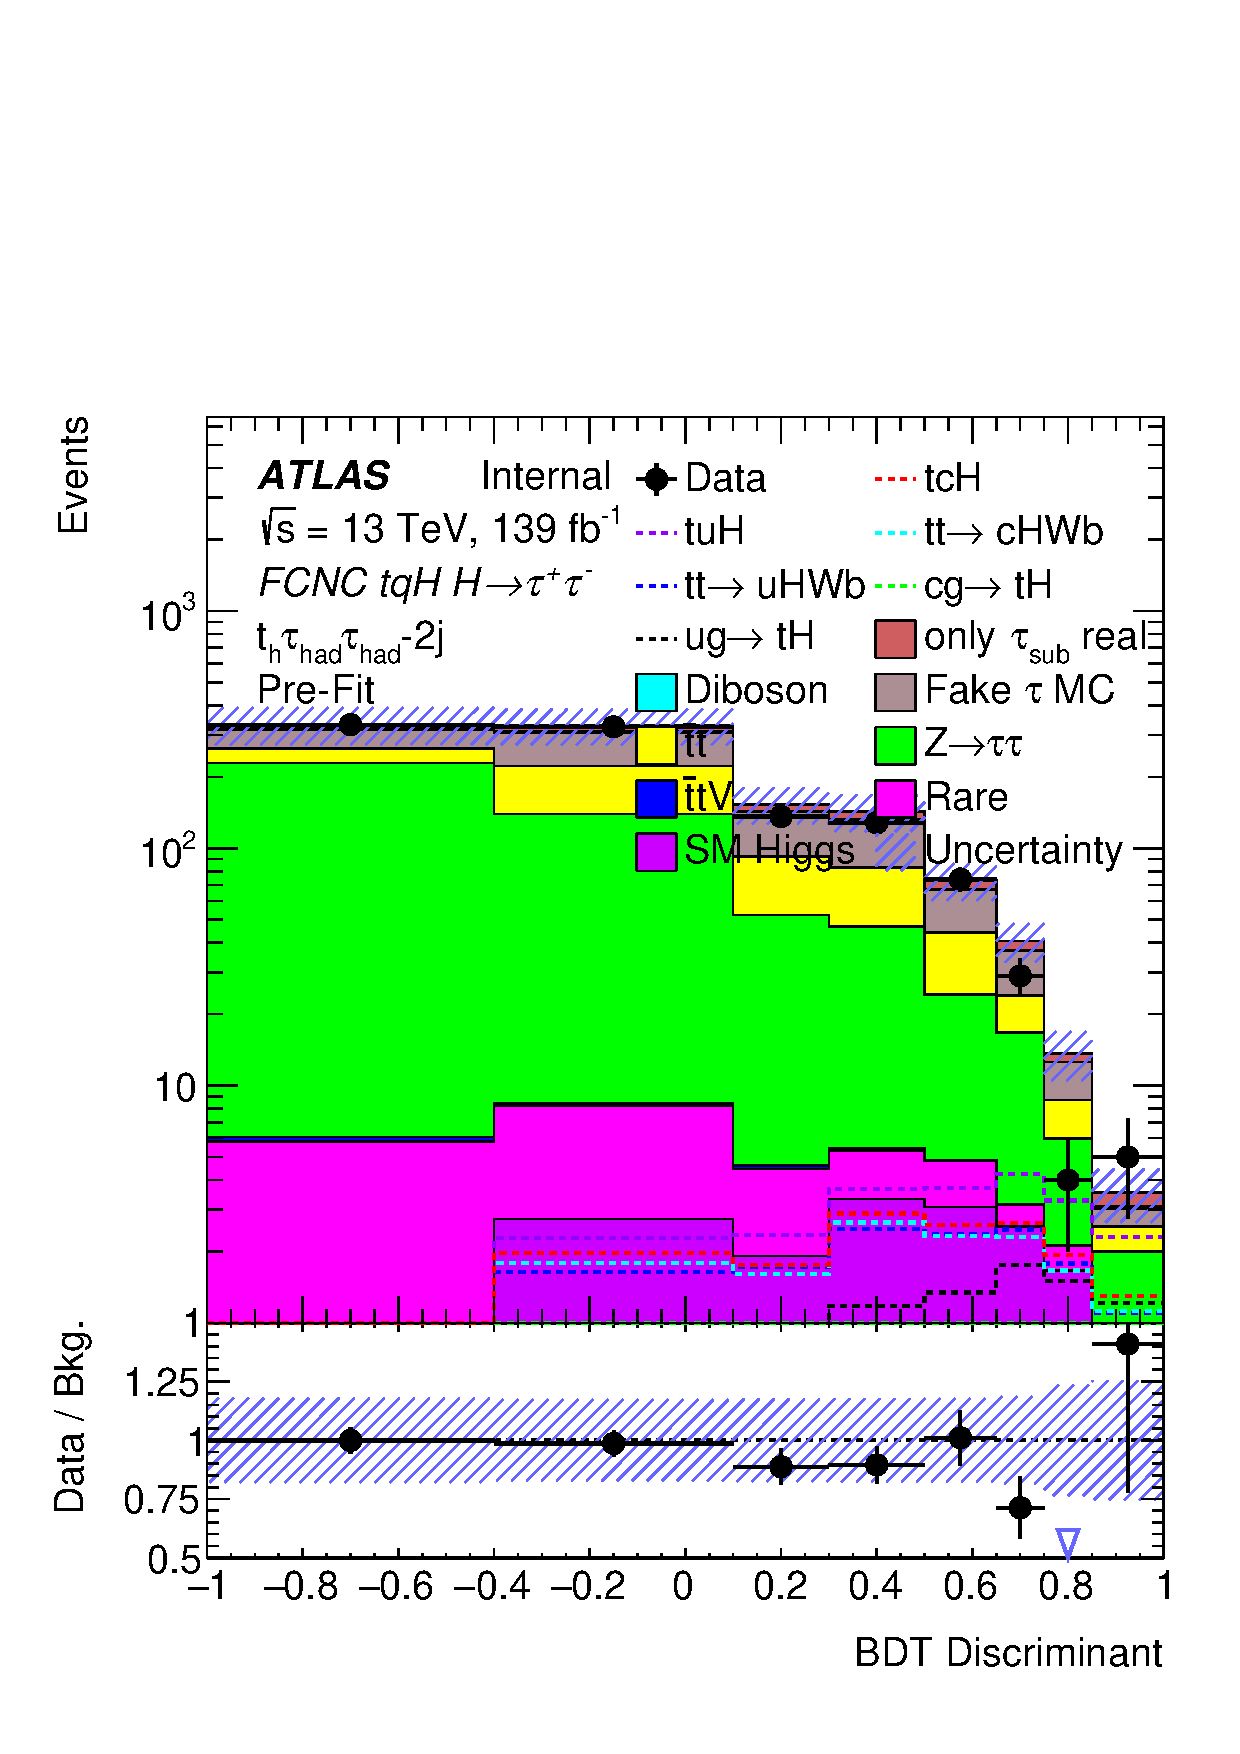
\includegraphics[width=0.33\textwidth]{figures/reg2mtau1b2jos_vetobtagwp70_highmet_pre_bonly.pdf}\\
% (b1) BDT in $t_h\tlhad$-2j & (b2) BDT in $t_h\tlhad$-3j & (b3) BDT in $t_h\thadhad$-2j \\
%   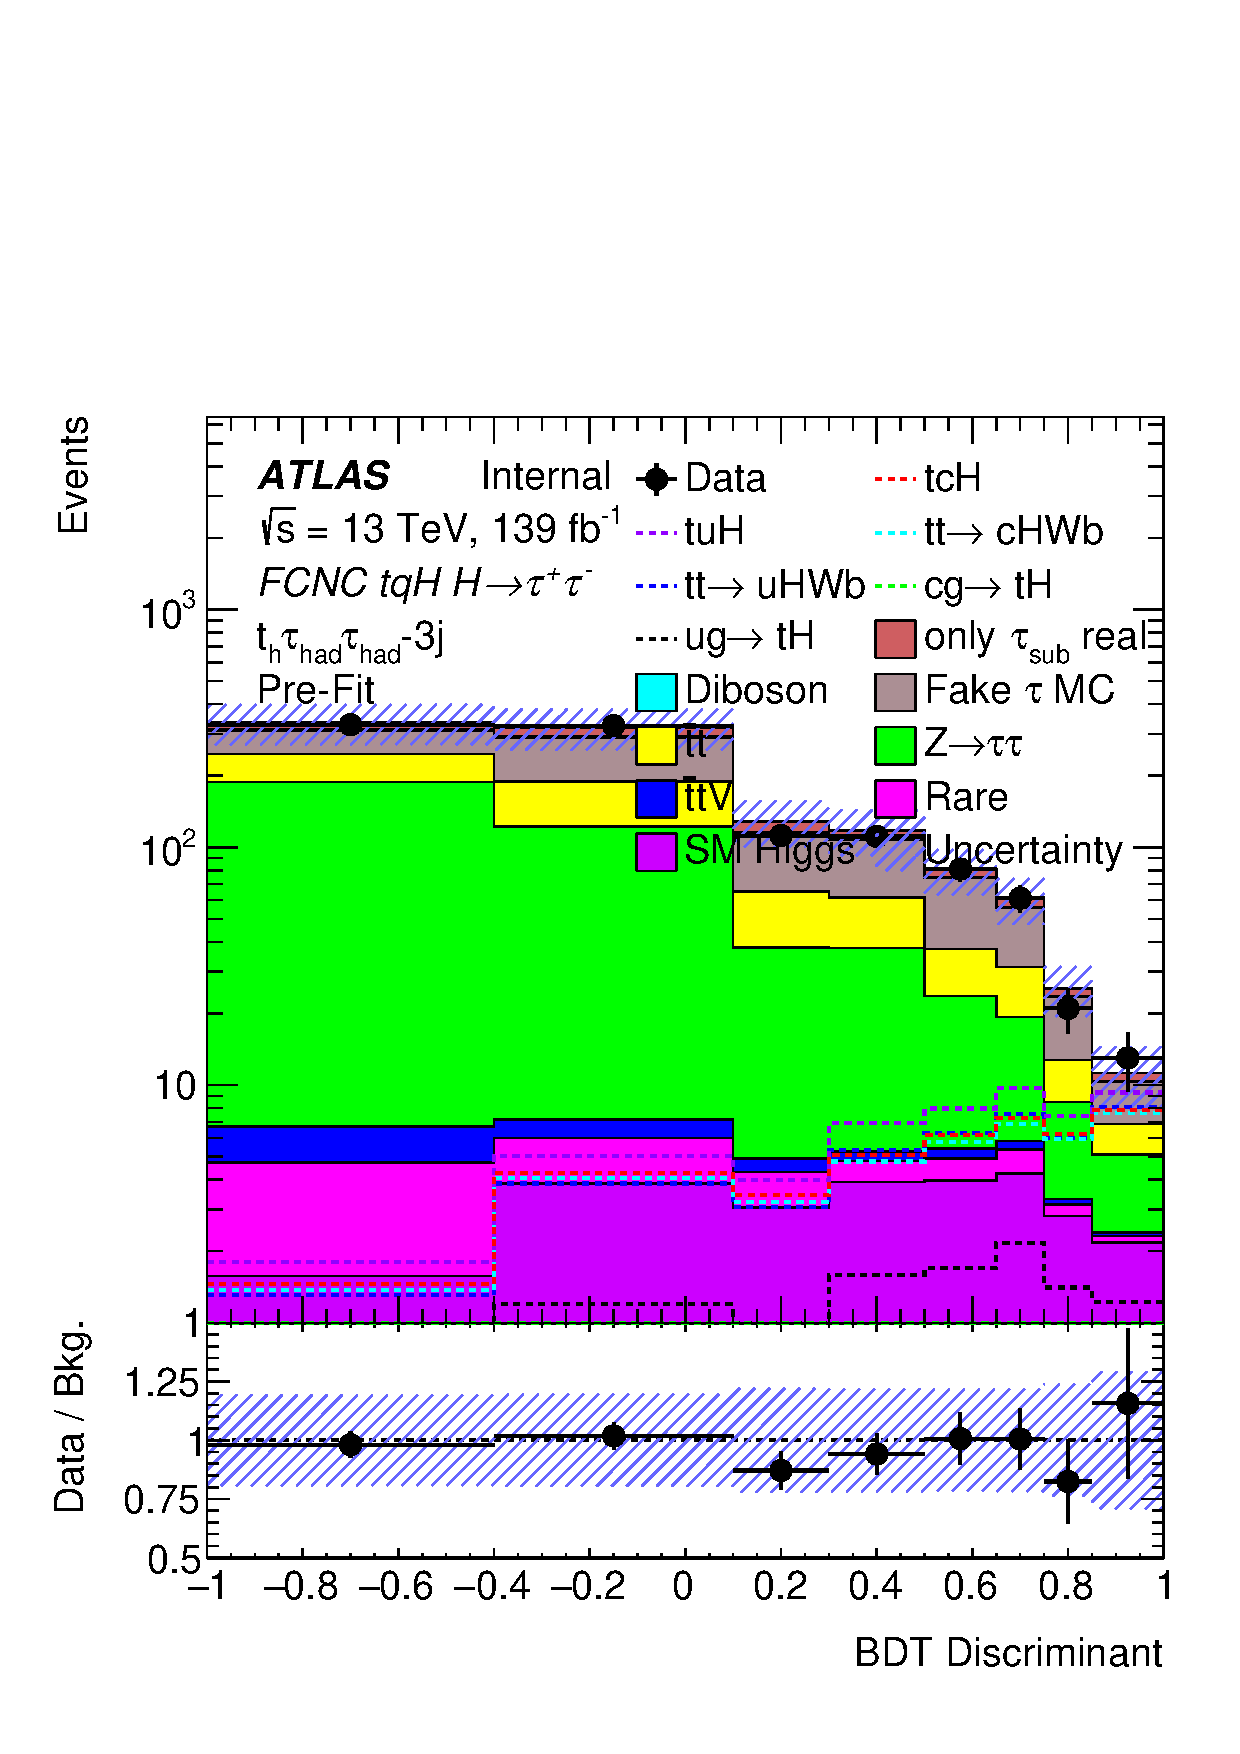
\includegraphics[width=0.33\textwidth]{figures/reg2mtau1b3jos_vetobtagwp70_highmet_pre_bonly.pdf}& \\
% (c1) BDT in$t_h\thadhad$-3j\\
% \end{tabular}
% \caption{ The BDT output distributions are fitted with background only to the data: $t_{\ell}\thadhad$ (a1),  $t_{\ell}\tauhad$-1j (a2),  $t_{\ell}\tauhad$-2j (a3),
%   $t_h\tlhad$-2j (b1), $t_h\tlhad$-3j (b2), $t_h\thadhad$-2j (b3), and $t_h\thadhad$-3j (c1).
%   Statistical and systematic uncertainties are being shown. For different type of signals are also shown for comparing their shapes. ({\textbf to be updated?})}
% \label{fig:Bonlyfit_data}
% \end{figure}



%\input{\FCNCFigures/tex/tthML_trexPrefit}
%\input{\FCNCFigures/tex/xTFW_trexPrefit}
\begin{figure}[H]
\centering
%\begin{tabular}{@{}ccc@{}}
%\includegraphics[width=0.33\textwidth]{\FCNCFigures/tthML/Limit/tcH_reg1l2tau1bnj_os_postFit.pdf}&
%\includegraphics[width=0.33\textwidth]{\FCNCFigures/tthML/Limit/tcH_reg1l1tau1b1j_ss_postFit.pdf}&
%\includegraphics[width=0.33\textwidth]{\FCNCFigures/tthML/Limit/tcH_reg1l1tau1b2j_ss_postFit.pdf}\\
%(a1) BDT discriminant in $t_{\ell}\thadhad$ & (a2) BDT discriminant in  $t_{\ell}\tauhad$-1j& (a3) BDT discriminant in $t_{\ell}\tauhad$-2j\\
%\includegraphics[width=0.33\textwidth]{\FCNCFigures/tthML/Limit/tcH_reg1l1tau1b2j_os_postFit.pdf}&
%\includegraphics[width=0.33\textwidth]{\FCNCFigures/tthML/Limit/tcH_reg1l1tau1b3j_os_postFit.pdf}&
%\includegraphics[width=0.33\textwidth]{\FCNCFigures/xTFW/Limit/tcH_reg2mtau1b2jos_vetobtagwp70_highmet_postFit.pdf}\\
%(b1) BDT discriminant in $t_h\tlhad$-2j & (b2) BDT discriminant in  $t_h\tlhad$-3j & (b3) BDT discriminant in $t_h\thadhad$-2j \\
%\includegraphics[width=0.33\textwidth]{\FCNCFigures/xTFW/Limit/tcH_reg2mtau1b3jos_vetobtagwp70_highmet_postFit.pdf}& \\
%(c1) BDT discriminant in$t_h\thadhad$-3j\\
%\end{tabular}
%\caption{ The BDT output distributions are fitted to the asimov S+B data in $tHc$ search: $t_{\ell}\thadhad$ (a1),  $t_{\ell}\tauhad$-1j (a2),  $t_{\ell}\tauhad$-2j (a3),
%  $t_h\tlhad$-2j (b1), $t_h\tlhad$-3j (b2), $t_h\thadhad$-2j (b3), and $t_h\thadhad$-3j (c1). Statistical and systematic uncertainties are being shown.}
%\label{fig:asimov_postfitbdtHc}


\begin{tabular}{@{}ccc@{}}
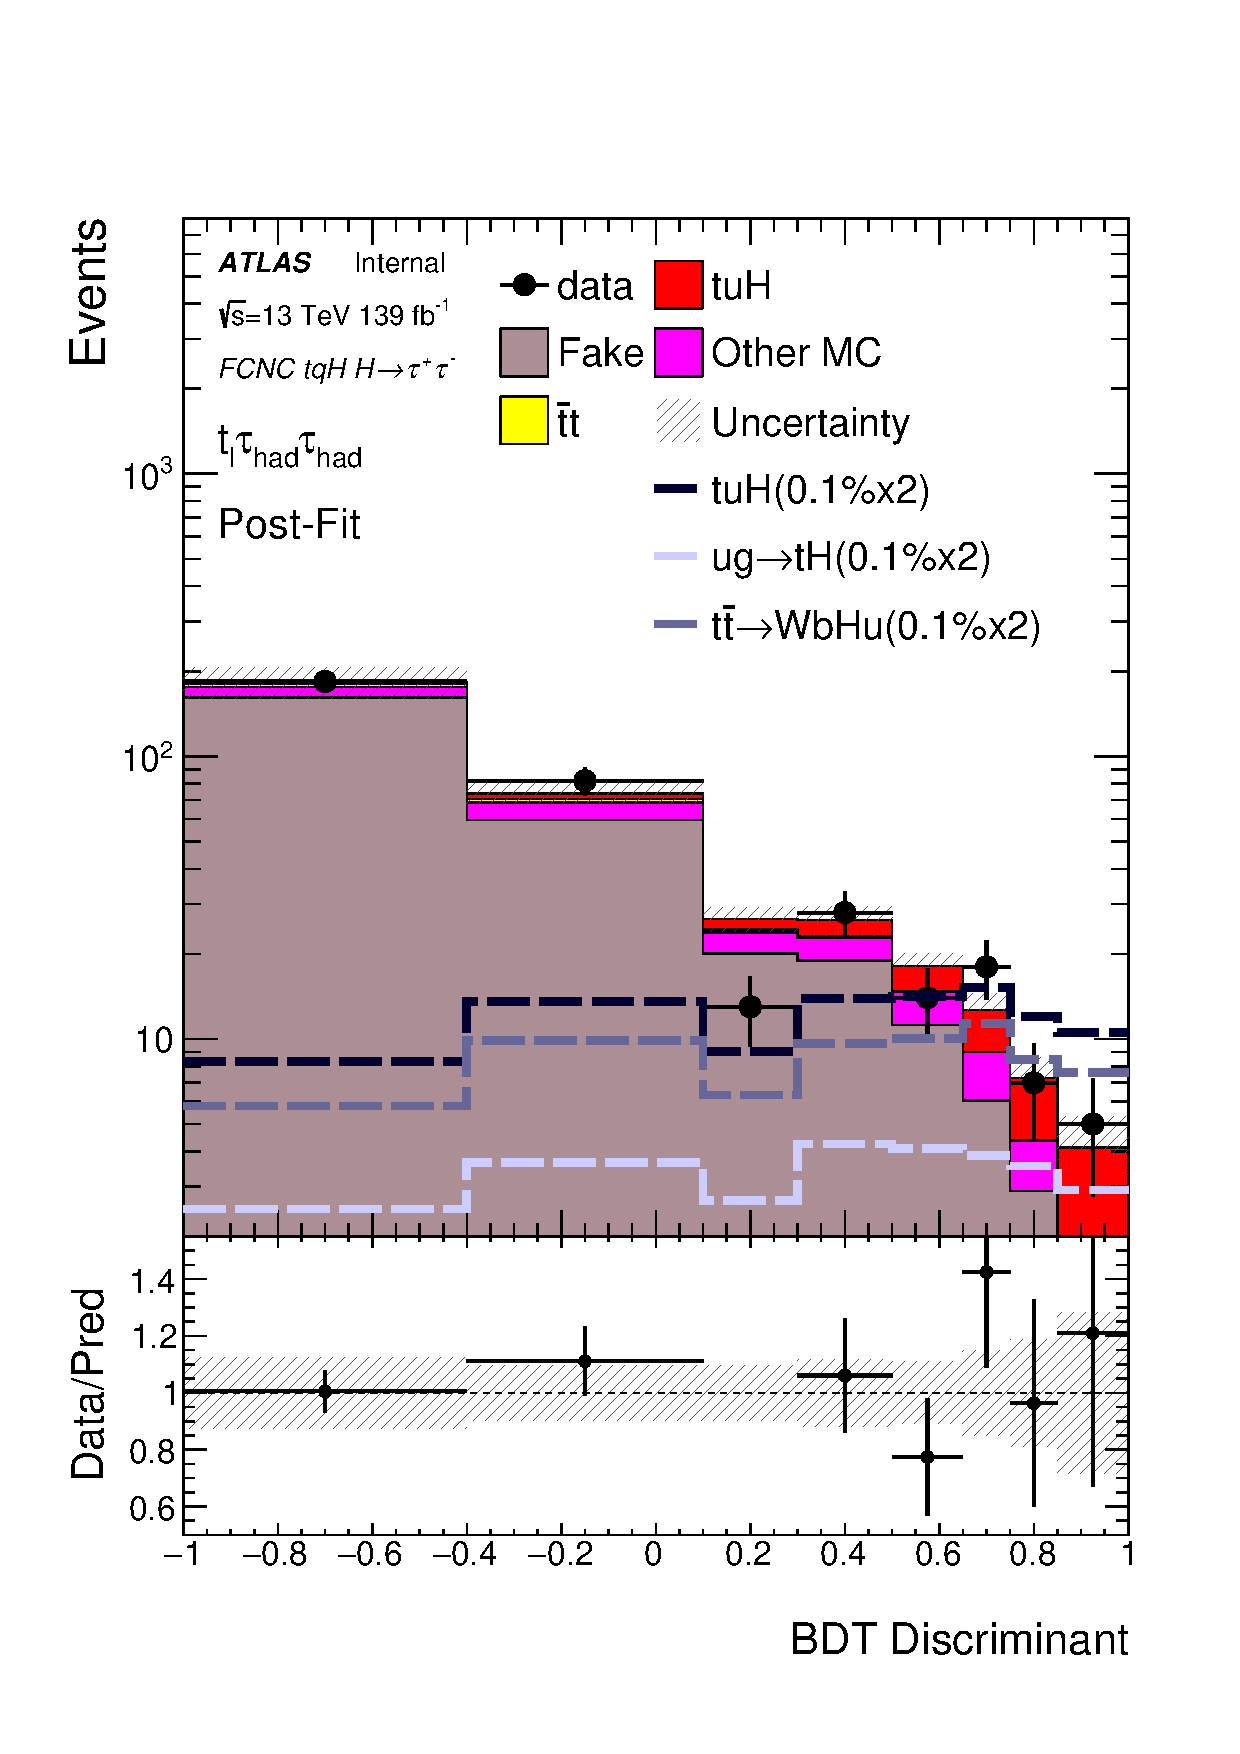
\includegraphics[width=0.29\textwidth]{figures/tuH_reg1l2tau1bnj_os.pdf}&
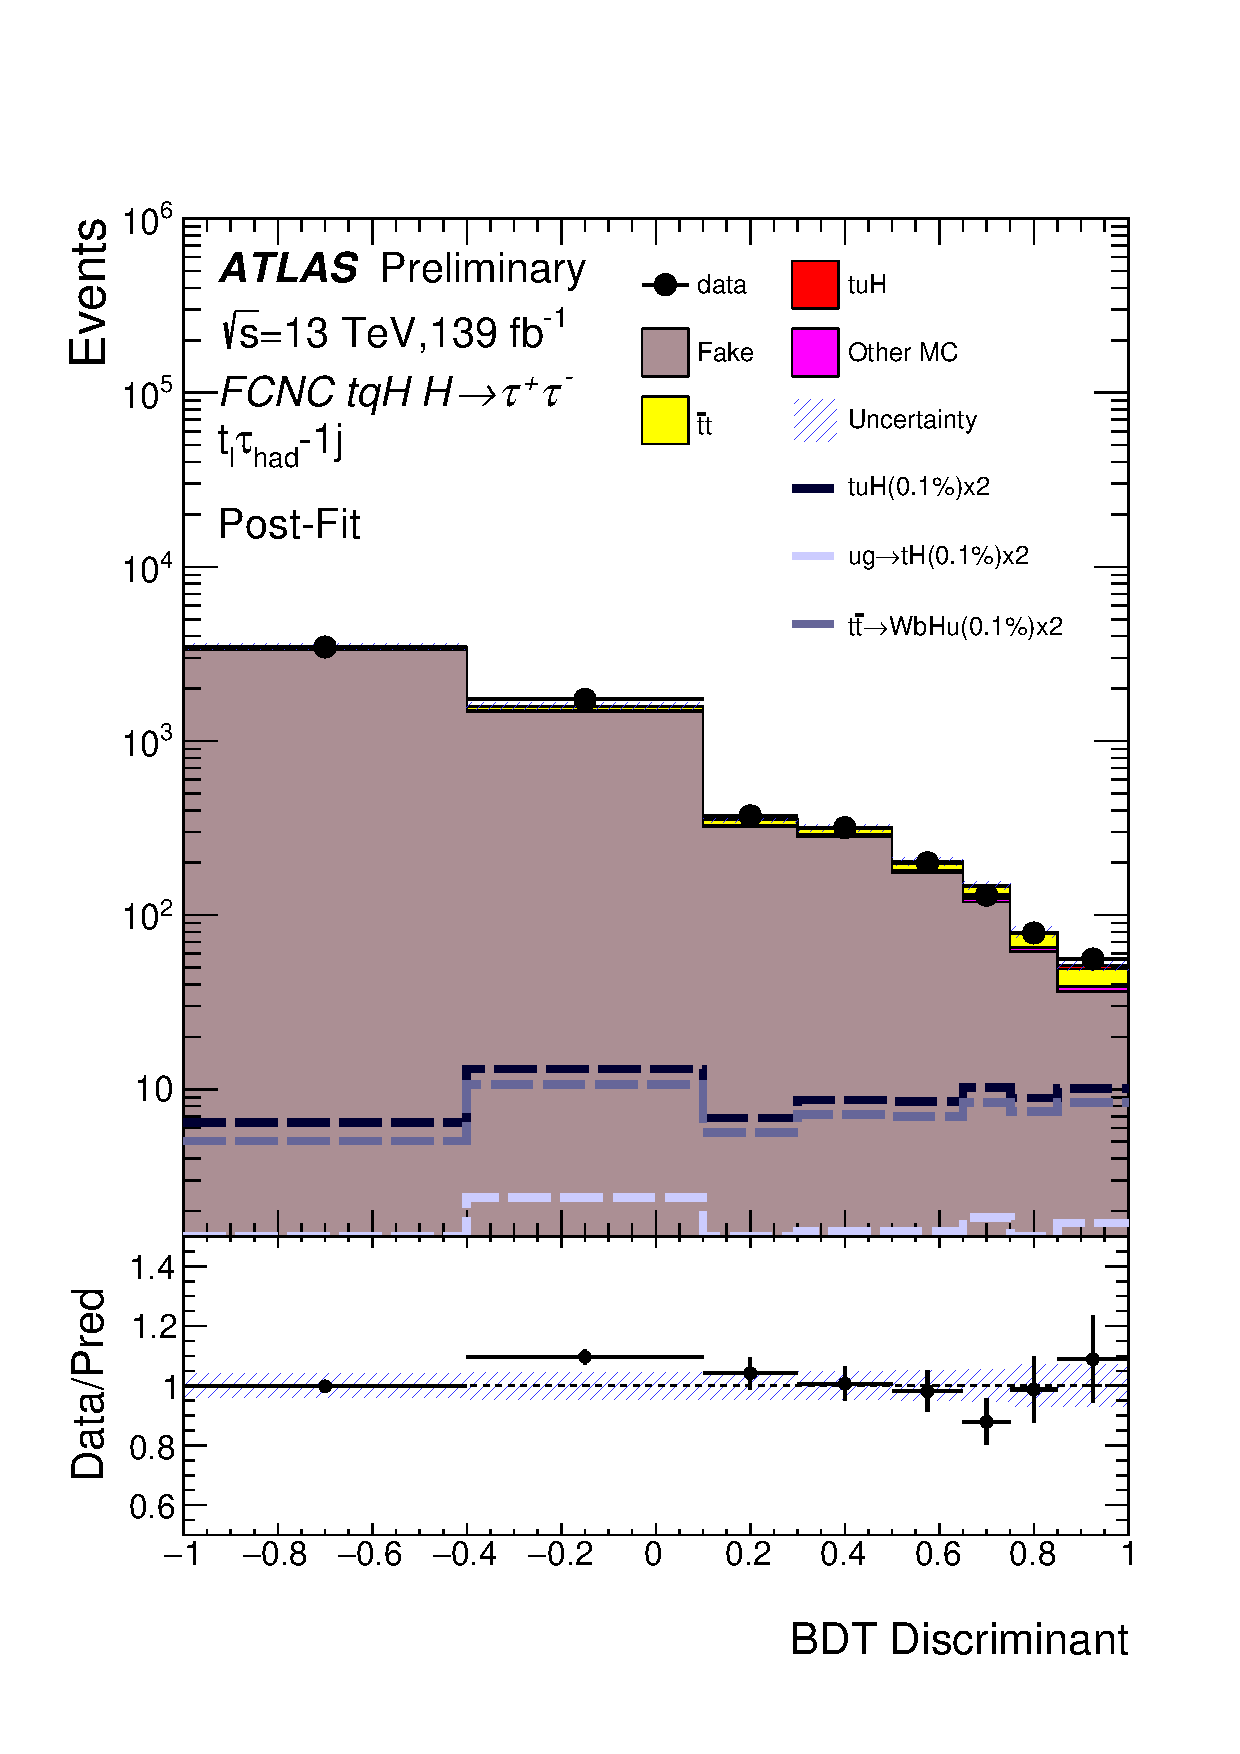
\includegraphics[width=0.29\textwidth]{figures/tuH_reg1l1tau1b1j_ss.pdf}&
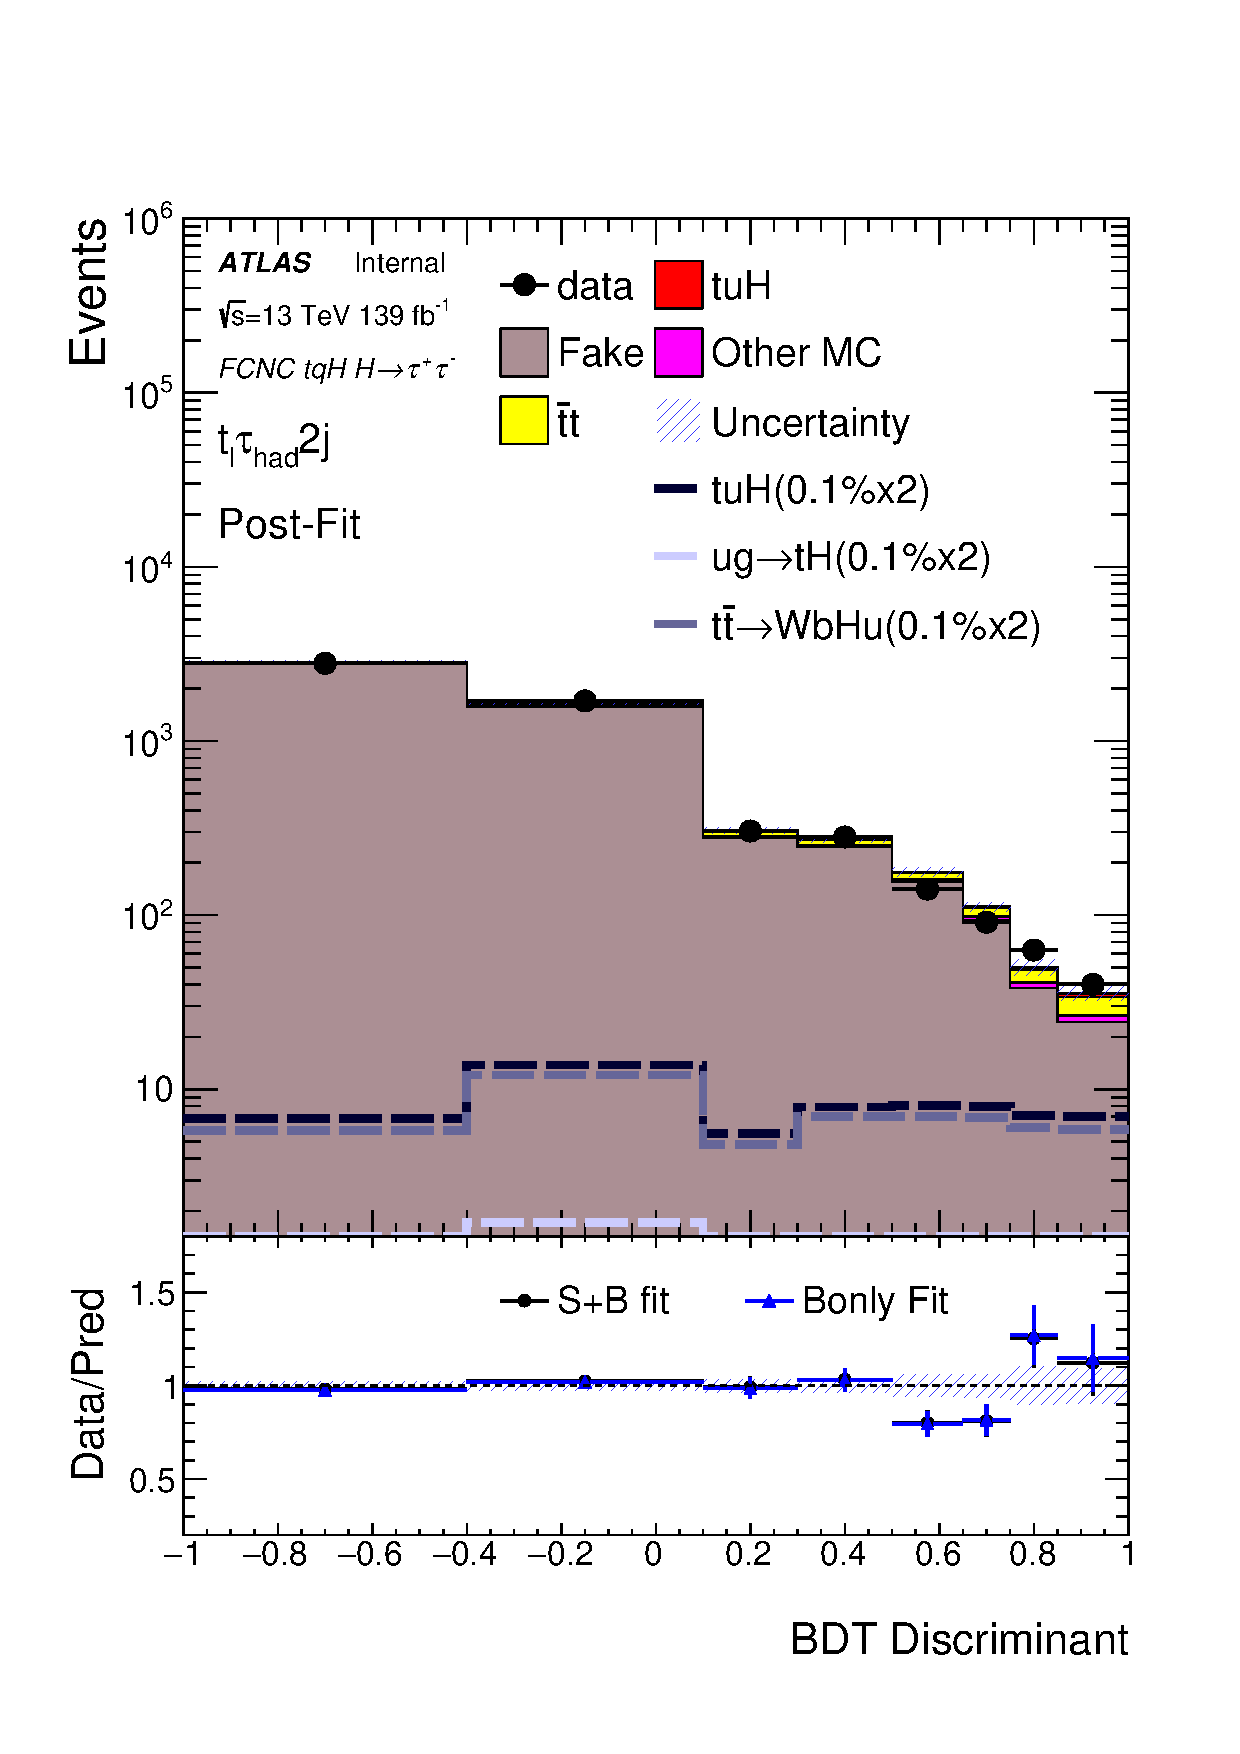
\includegraphics[width=0.29\textwidth]{figures/tuH_reg1l1tau1b2j_ss.pdf}\\
%(a1) BDT in $t_{\ell}\thadhad$ & (a2) BDT in  $t_{\ell}\tauhad$-1j& (a3) BDT in $t_{\ell}\tauhad$-2j\\
(a)  & (b) & (c) \\
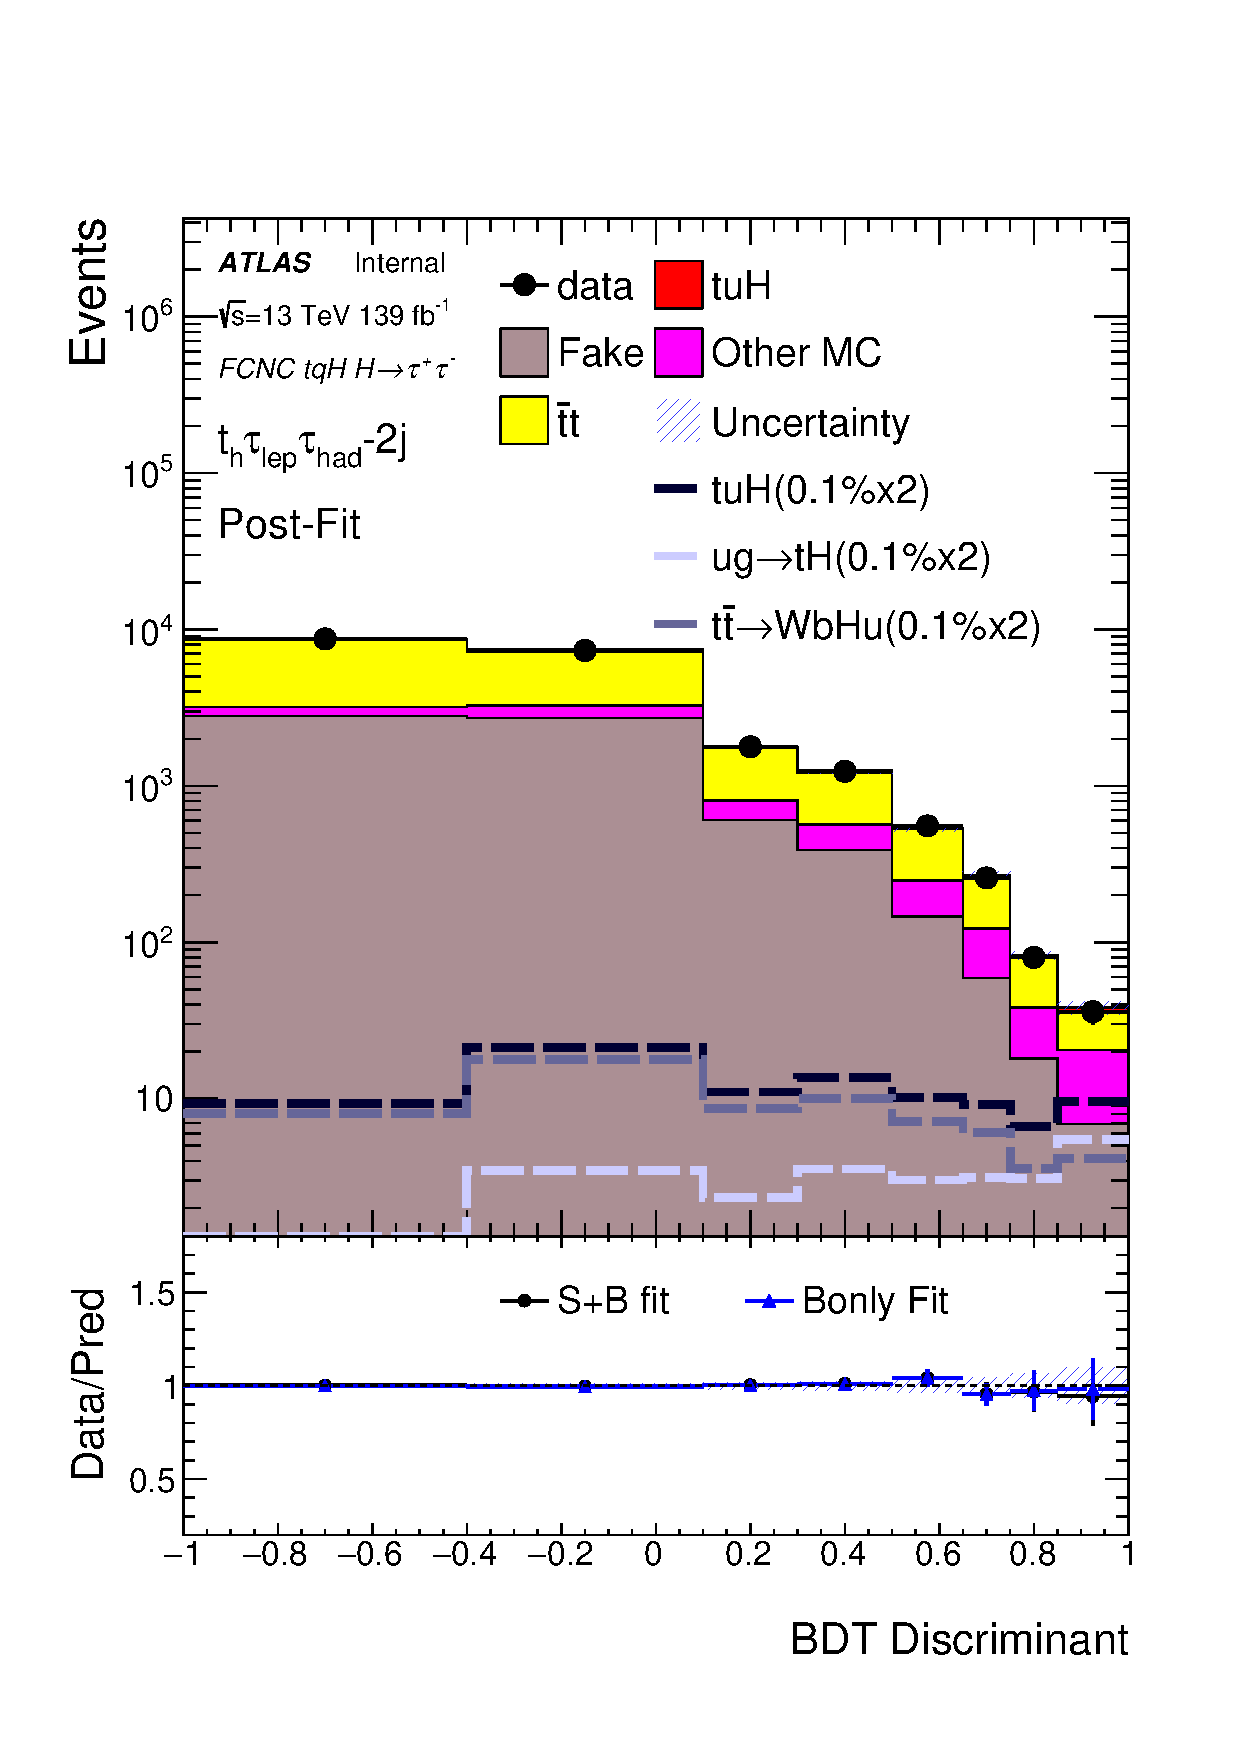
\includegraphics[width=0.29\textwidth]{figures/tuH_reg1l1tau1b2j_os.pdf}&
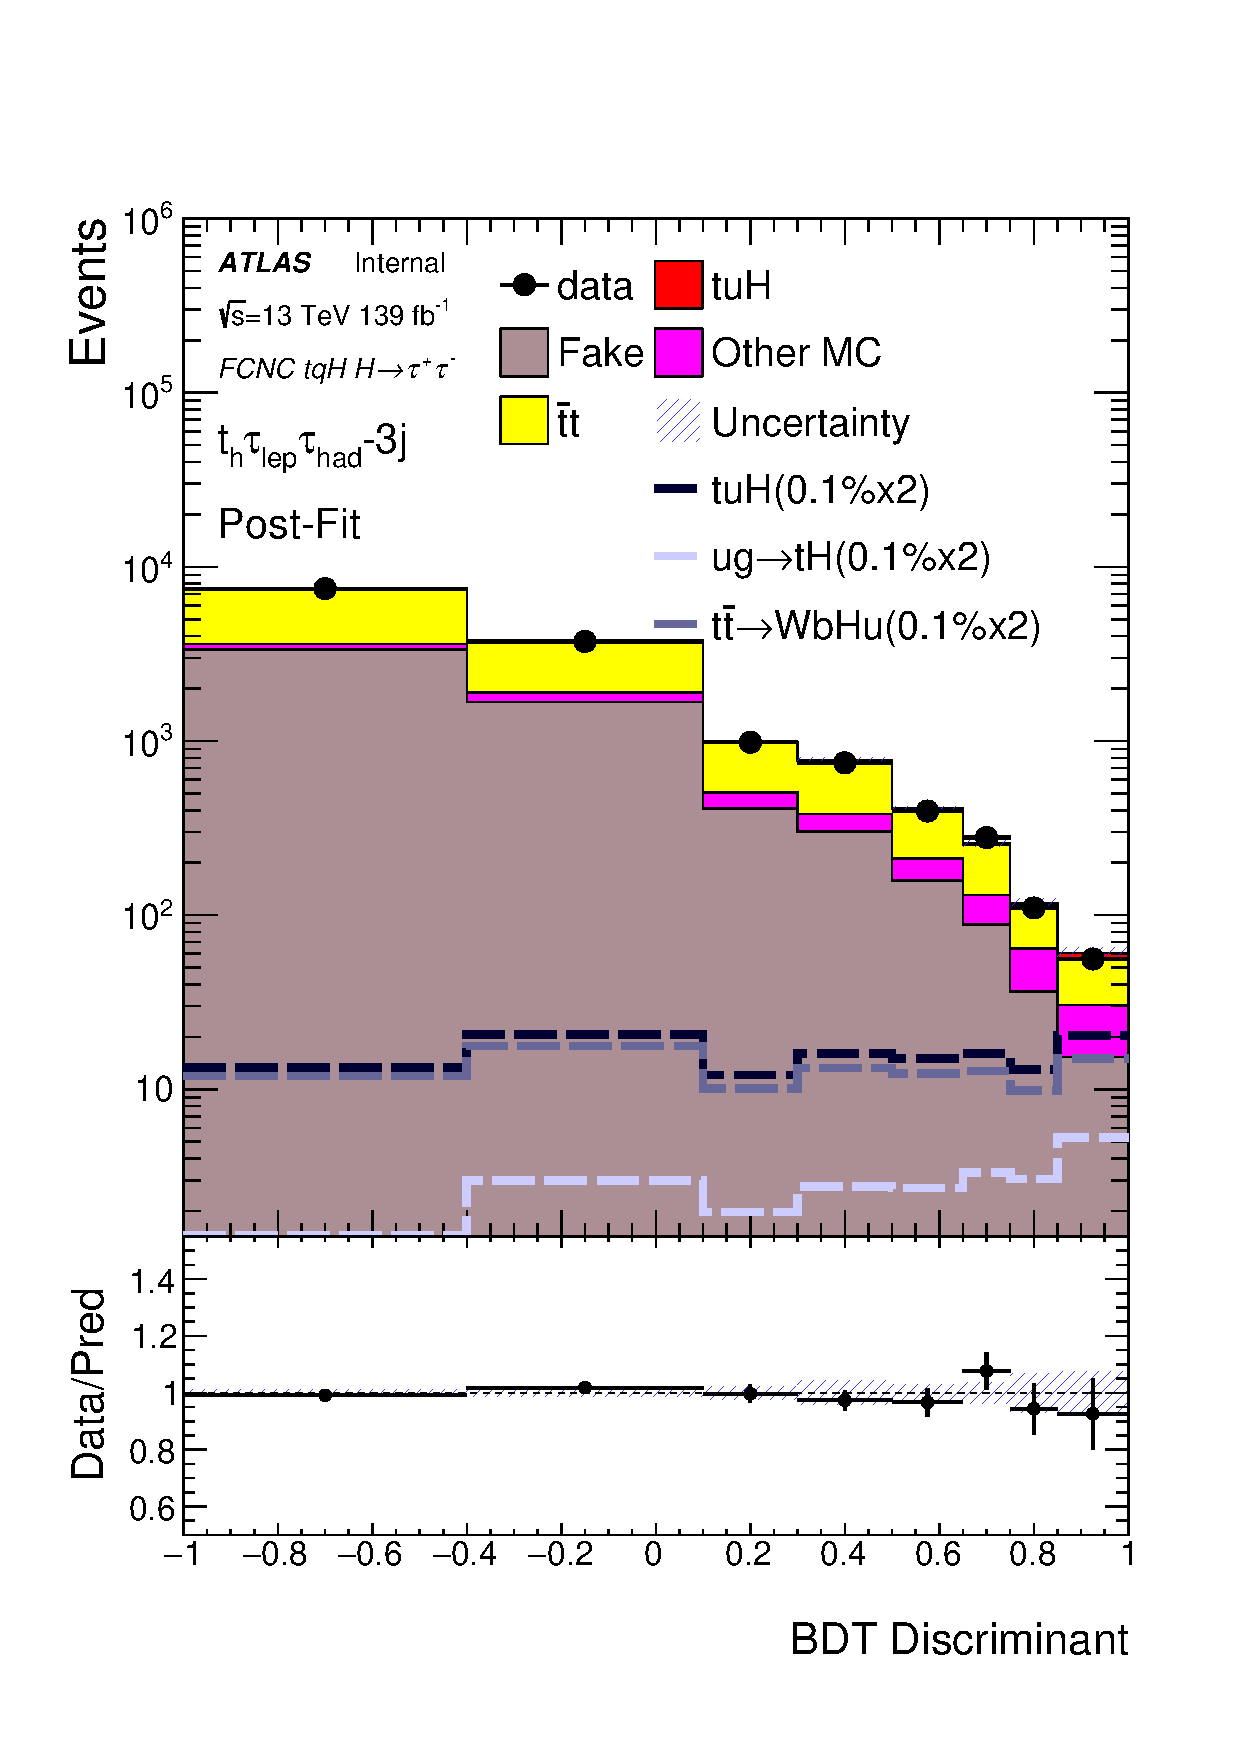
\includegraphics[width=0.29\textwidth]{figures/tuH_reg1l1tau1b3j_os.pdf}&
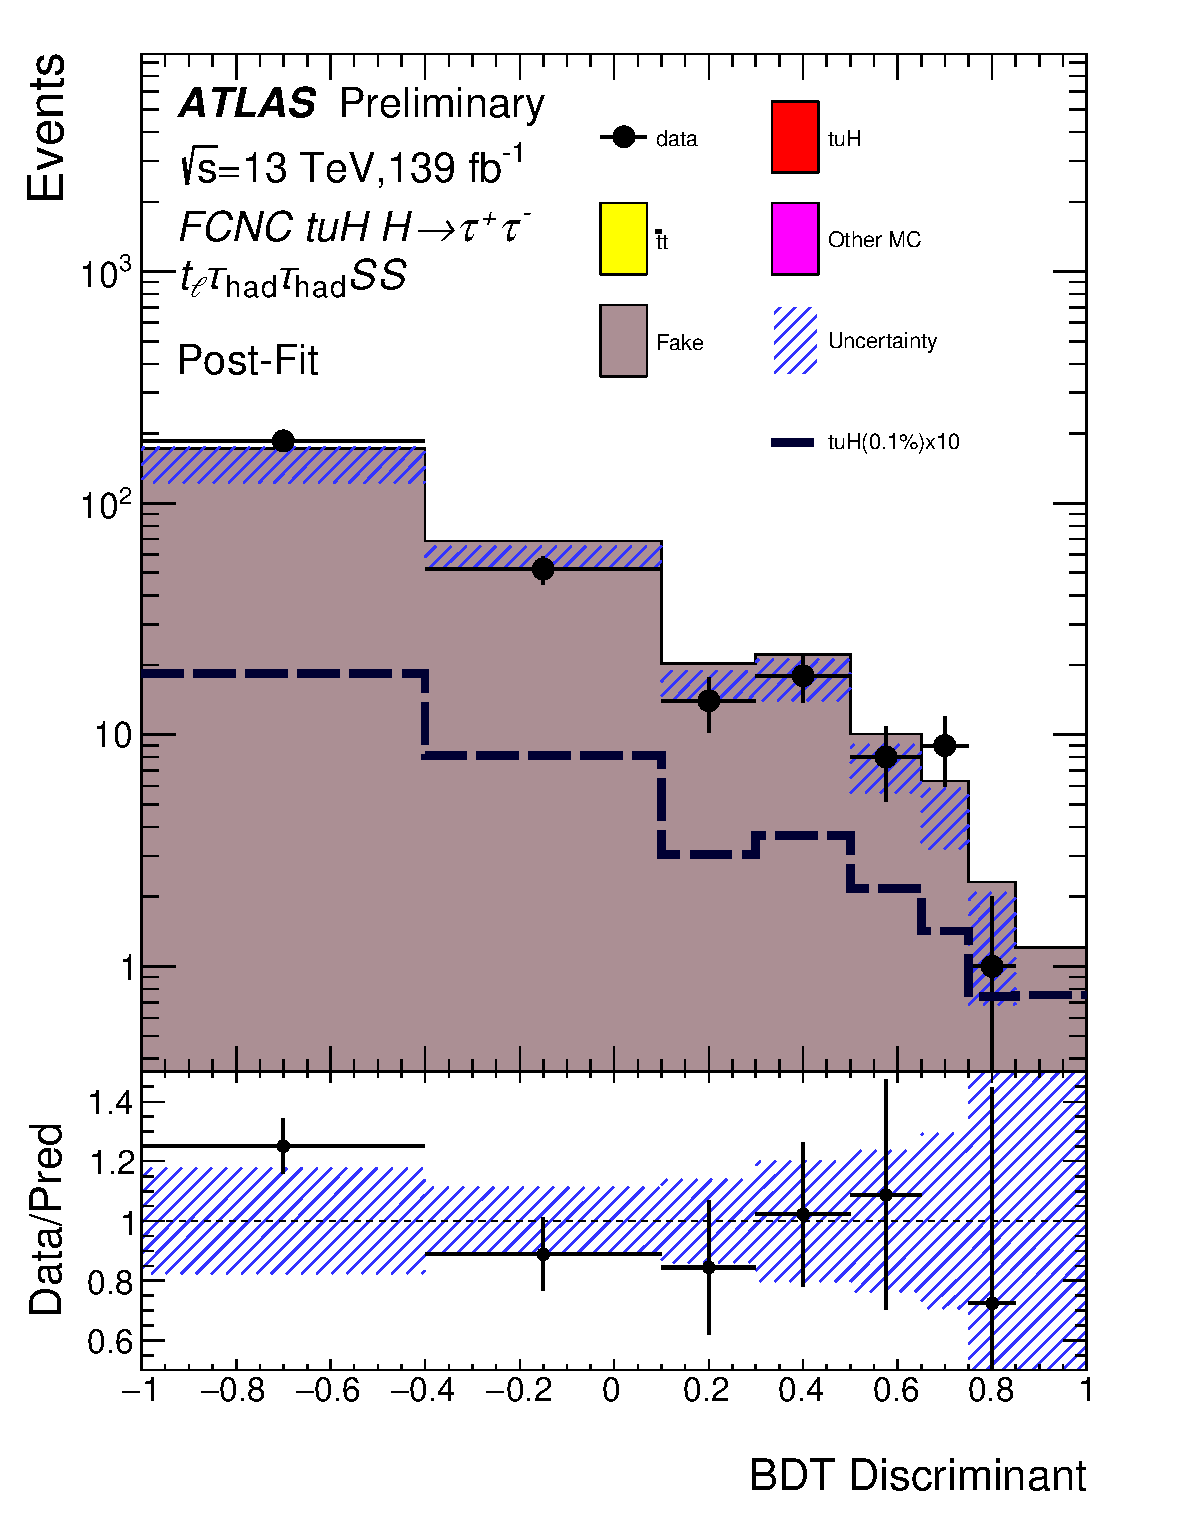
\includegraphics[width=0.29\textwidth]{figures/tuH_reg1l2tau1bnj_ss.pdf}\\
%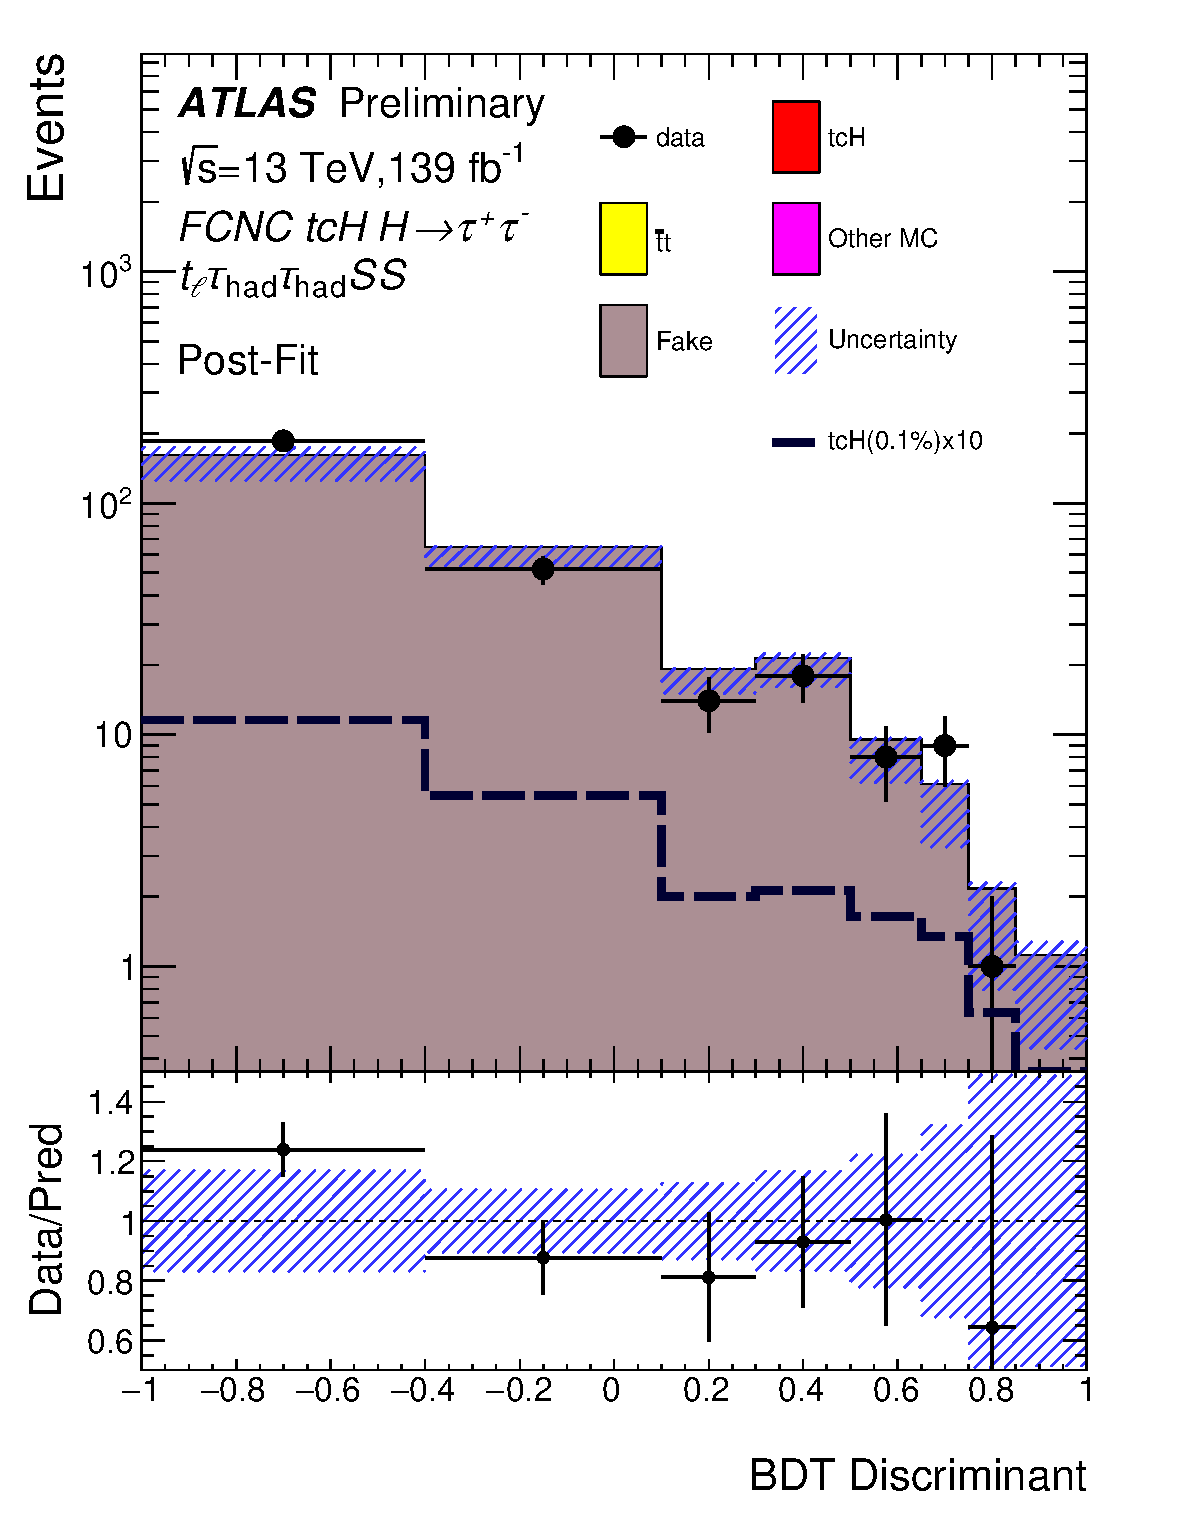
\includegraphics[width=0.3\textwidth]{figures/tcH_reg1l2tau1bnj_ss.pdf}\\
%(b1) BDT in $t_h\tlhad$-2j & (b2) BDT in  $t_h\tlhad$-3j & (b3) BDT in $t_h\thadhad$-2j \\
(d) & (e)  & (f) \\
%(d) & (e)\\
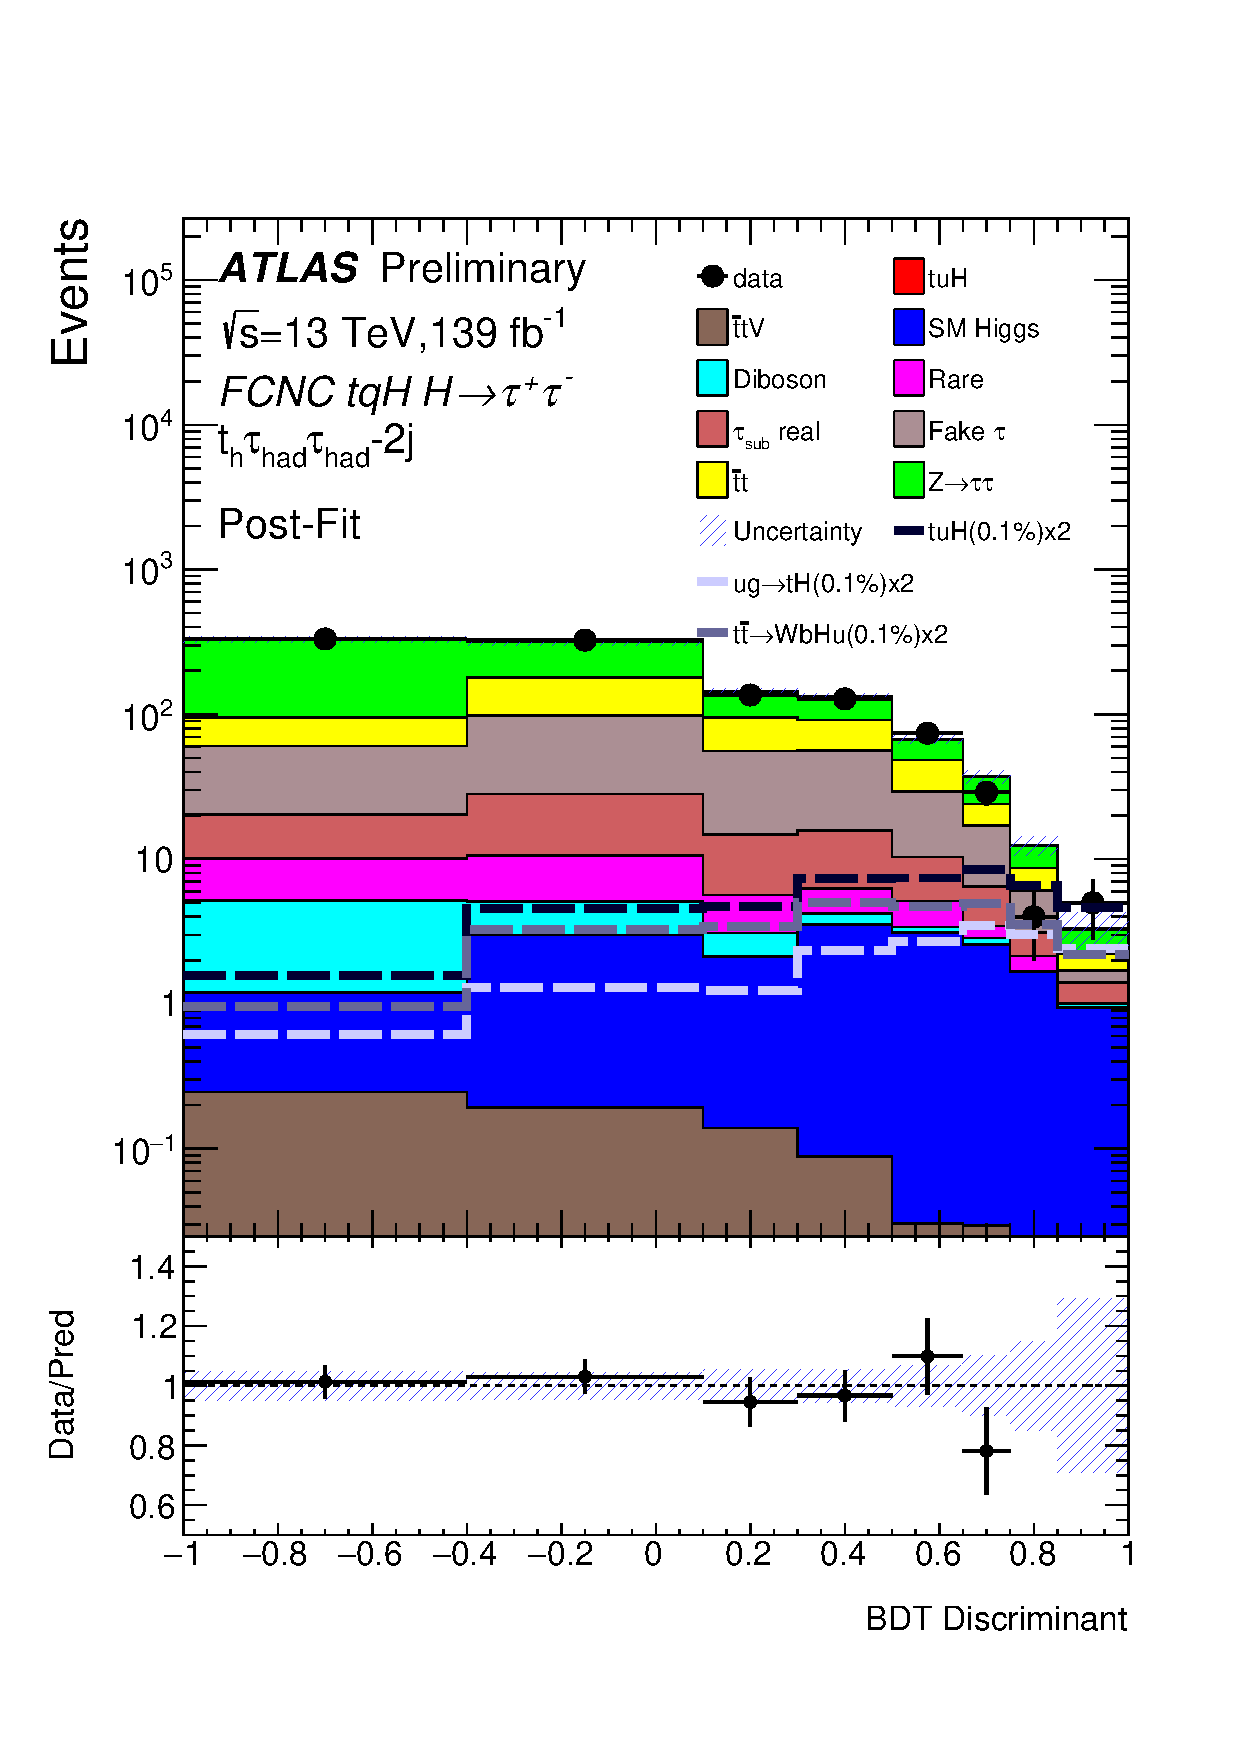
\includegraphics[width=0.29\textwidth]{figures/tuH_reg2mtau1b2jos.pdf}&
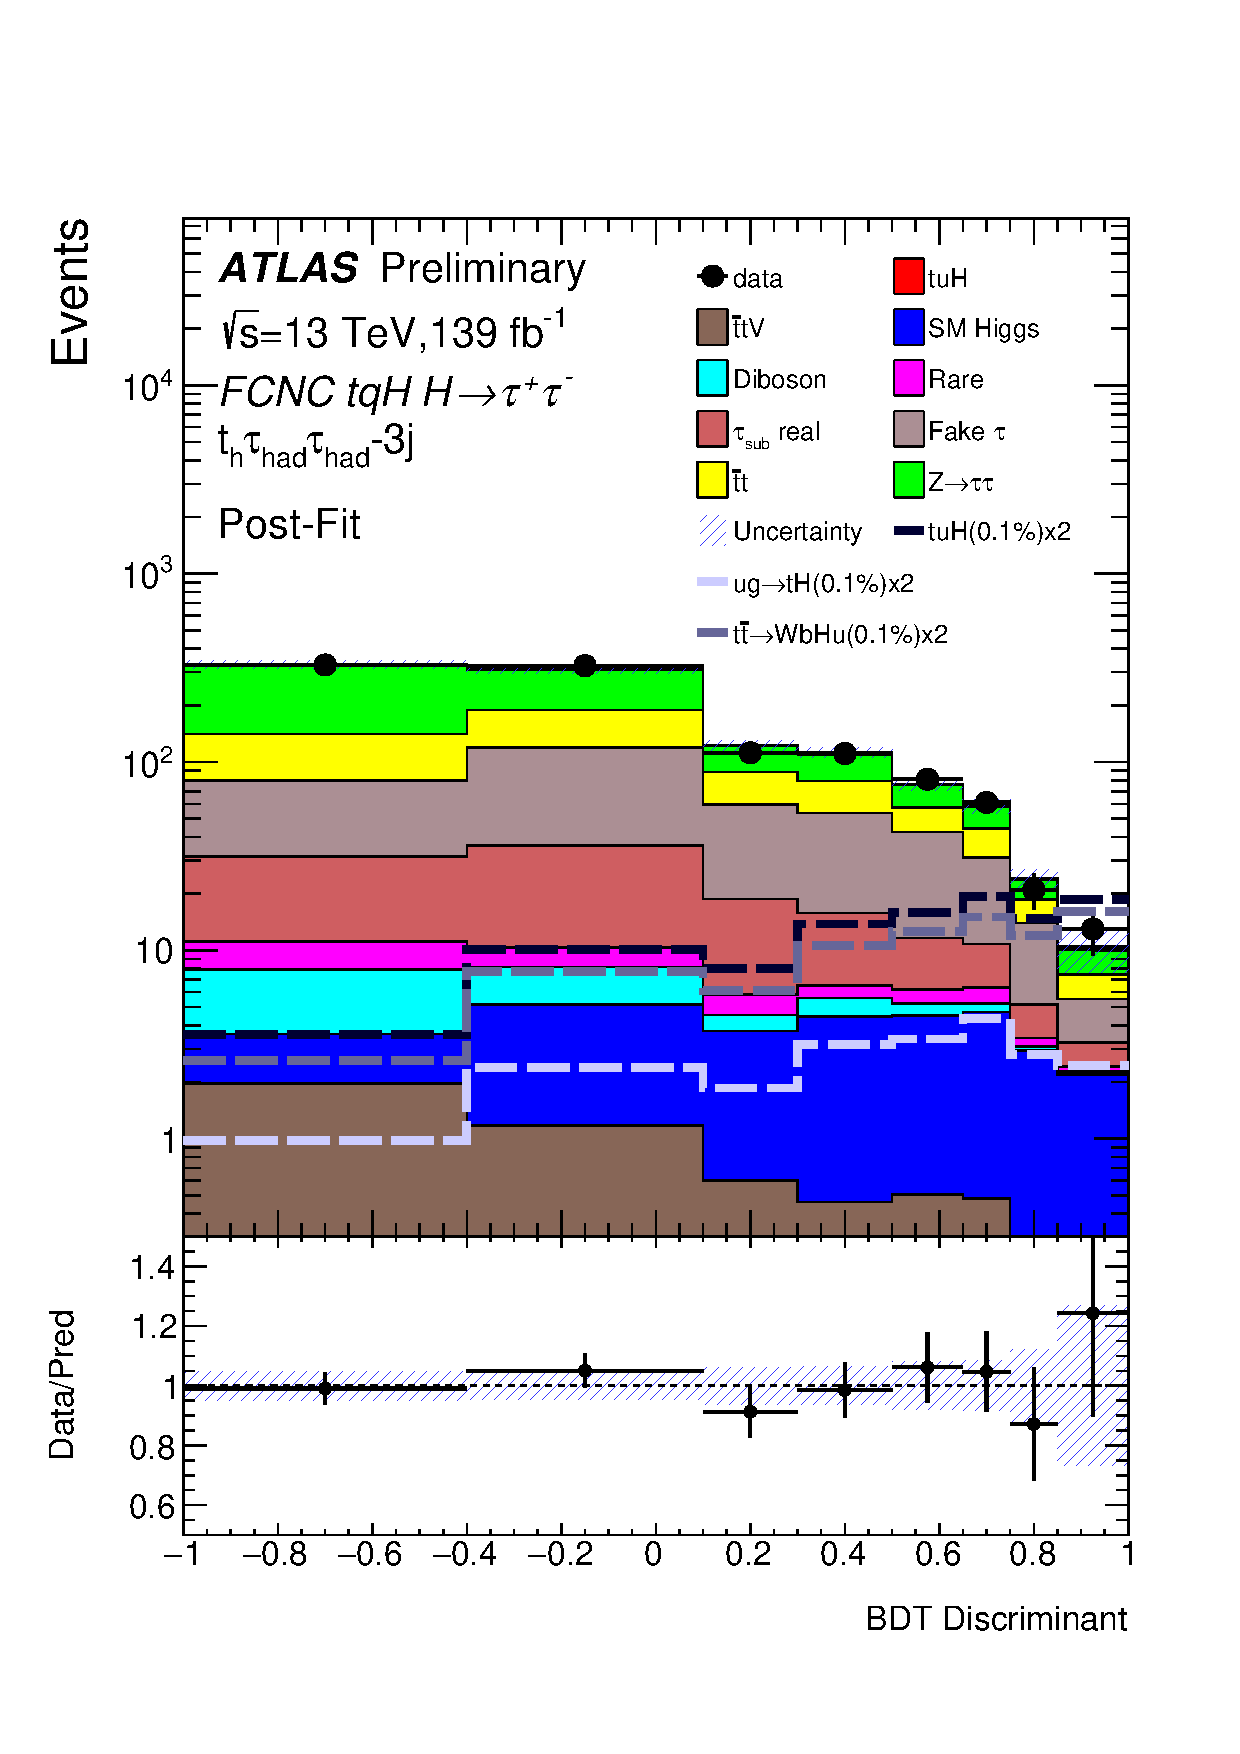
\includegraphics[width=0.29\textwidth]{figures/tuH_reg2mtau1b3jos.pdf}&
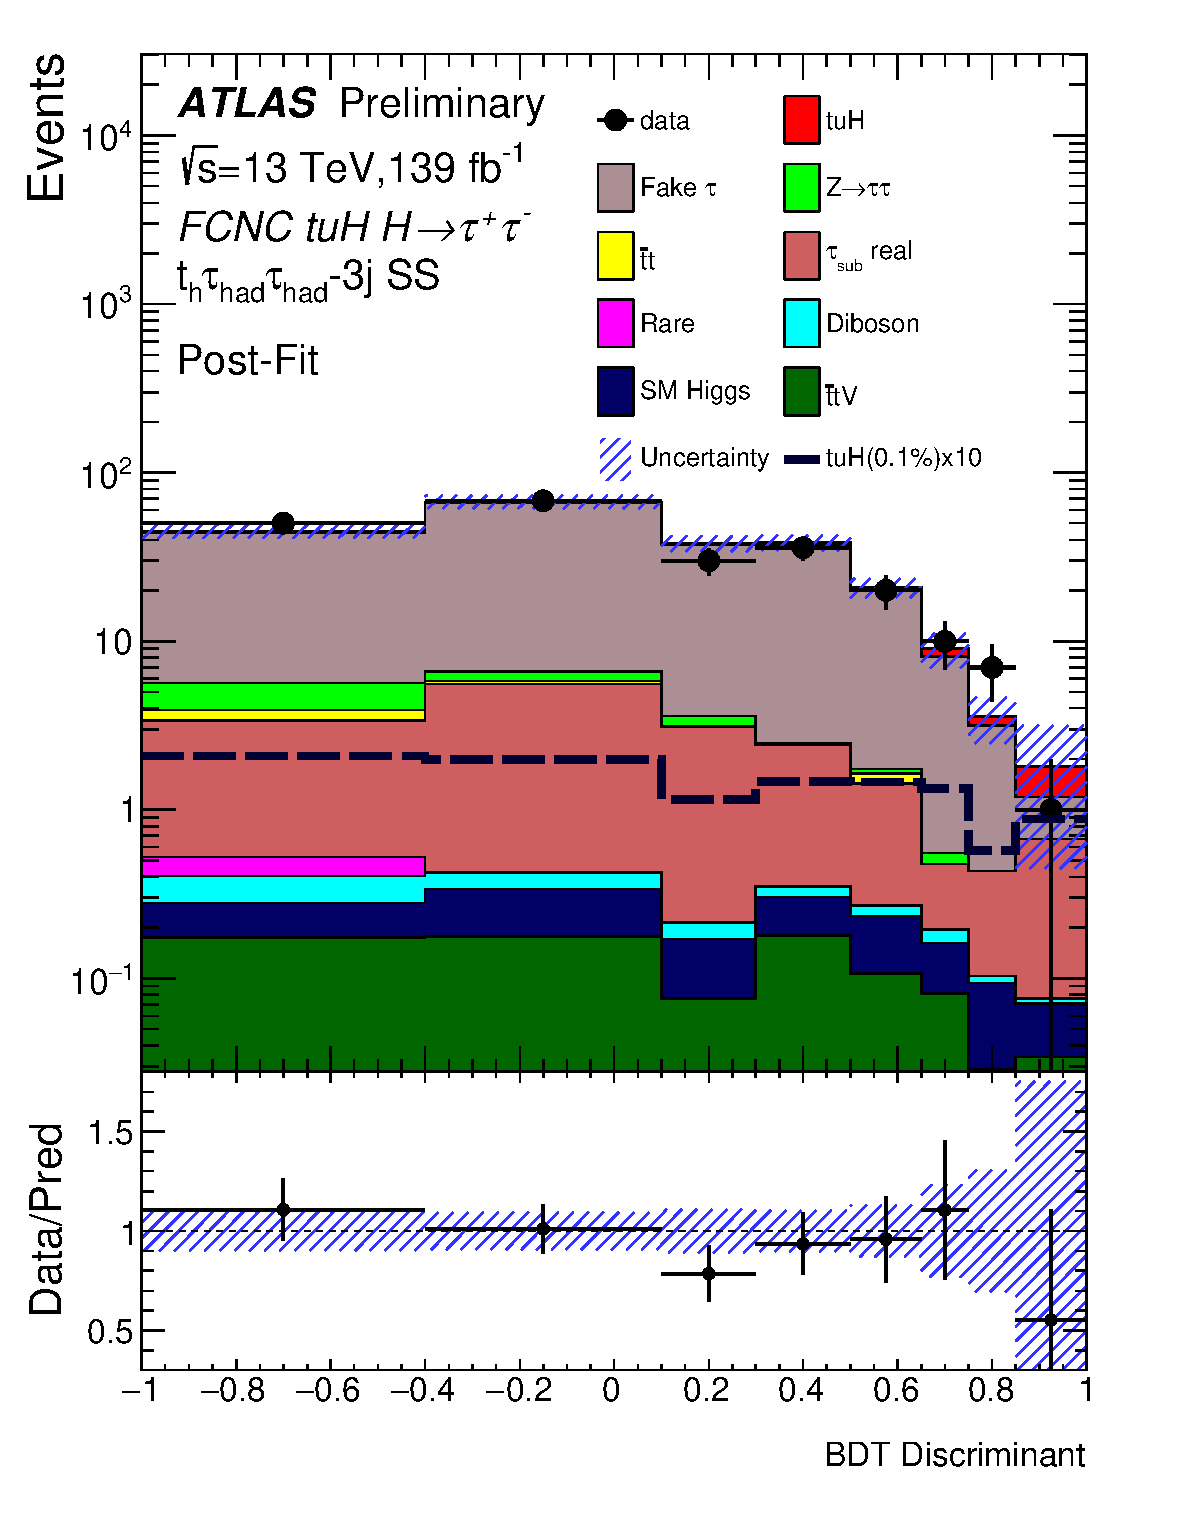
\includegraphics[width=0.29\textwidth]{figures/tuH_reg2mtau1b3jss.pdf}\\
%(c1) BDT in$t_h\thadhad$-3j\\
(g) & (h)  & (i) \\
%(f) & (g)  &  \\
\end{tabular}
\caption{ BDT output distributions obtained from a signal+background fit to the data for the $tuH$ search: 
%$t_{\ell}\thadhad$ (a),  $t_{\ell}\tauhad$-1j (b),  $t_{\ell}\tauhad$-2j (c), $t_h\tlhad$-2j (d), $t_h\tlhad$-3j (e), $t_{\ell}\thadhad$ SS (f), $t_h\thadhad$-2j (g), and $t_h\thadhad$-3j (h), where $t_{\ell}\thadhad$ SS is used for the background validation. 
(a) $t_{\ell}\thadhad$, (b) $t_{\ell}\tauhad$-1j,  (c) $t_{\ell}\tauhad$-2j, (d) $t_h\tlhad$-2j, (e) $t_h\tlhad$-3j, (f) $t_{\ell}\thadhad$-SS, (g) $t_h\thadhad$-2j, (h) $t_h\thadhad$-3j and (i) $t_h\thadhad$-3j SS.  
The total statistical and systematic uncertainty is indicated by the hatched band. The signal shapes of $tt(uH)$, $tH$, and their sum are also shown using a normalisation of $2 \times\BR(t\to uH)$ of 0.1\%. 
}
\label{fig:asimov_postfitbdtHu}
\end{figure}



\begin{figure}[H]
\centering
\begin{tabular}{@{}ccc@{}}
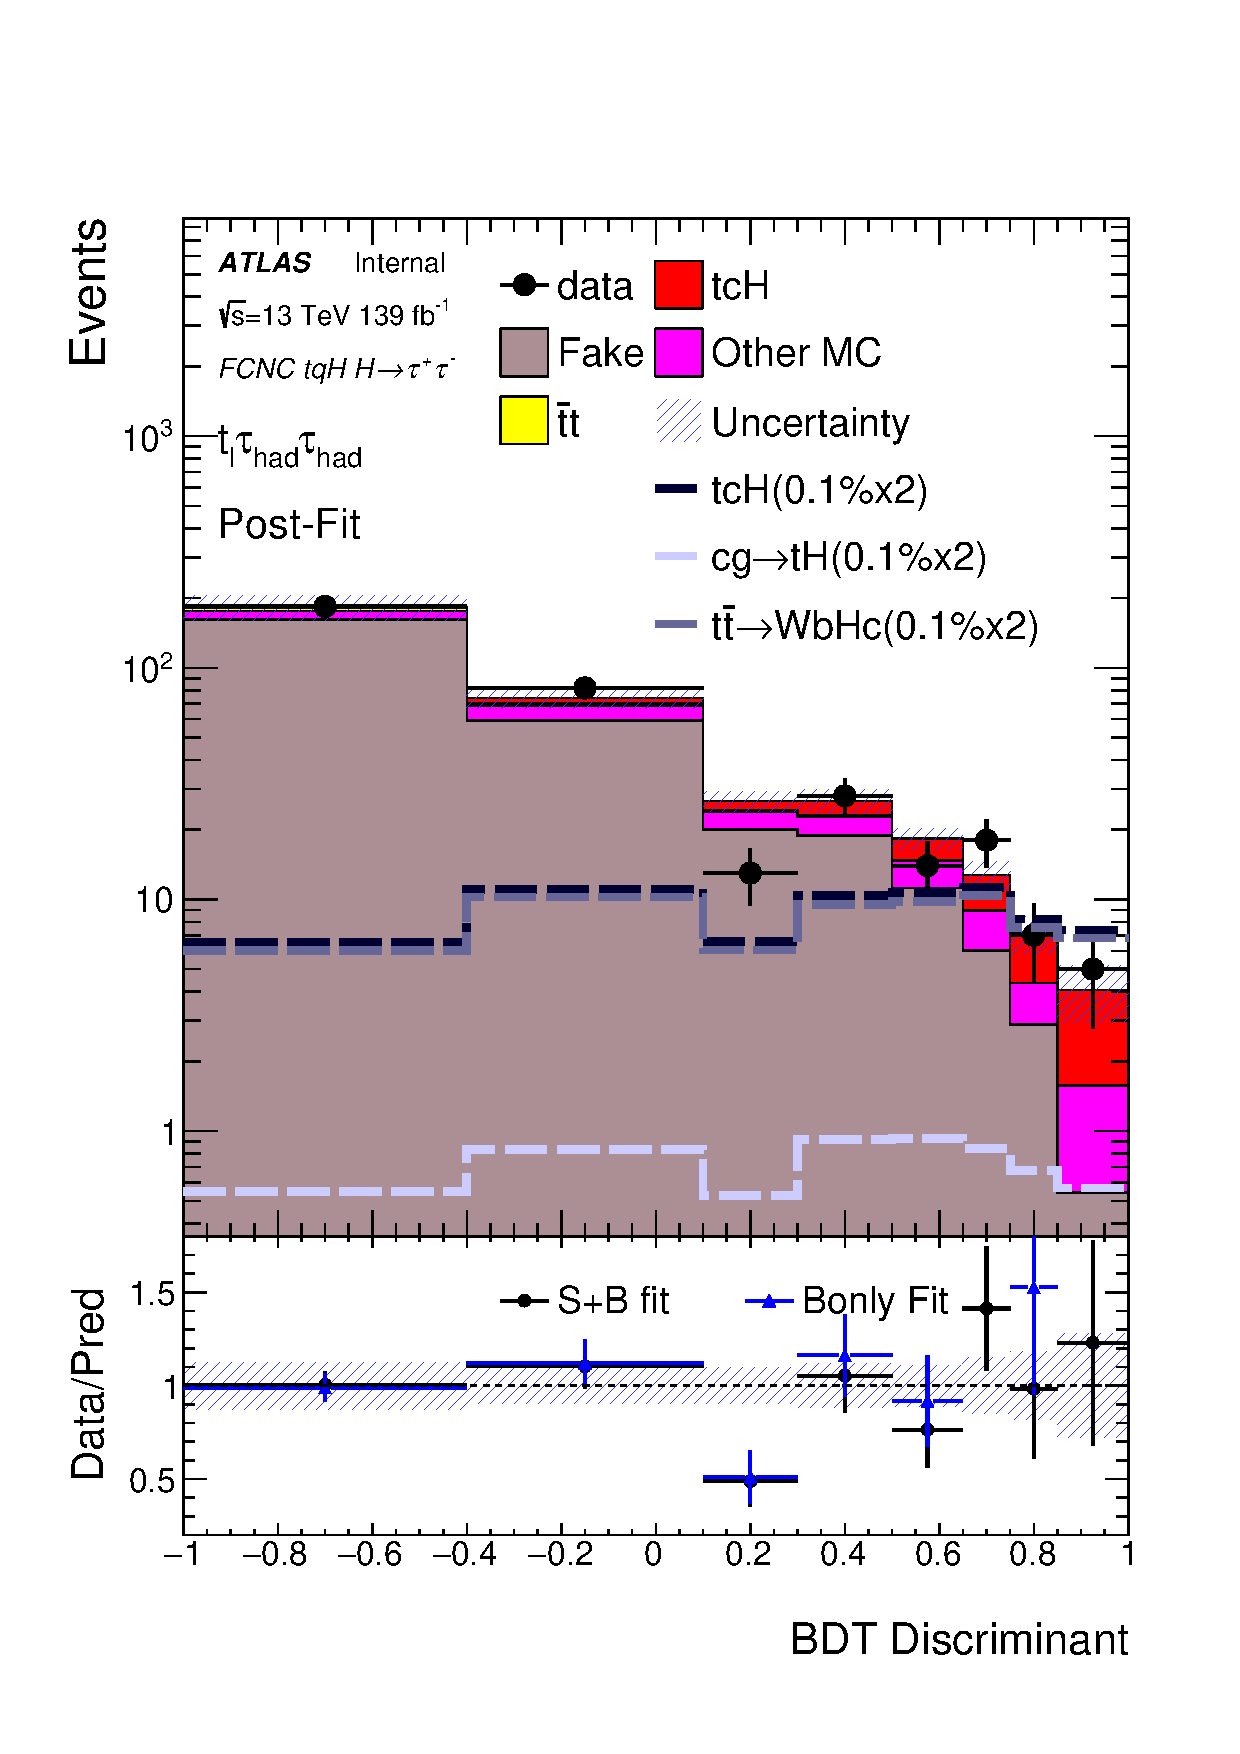
\includegraphics[width=0.29\textwidth]{figures/tcH_reg1l2tau1bnj_os.pdf}&
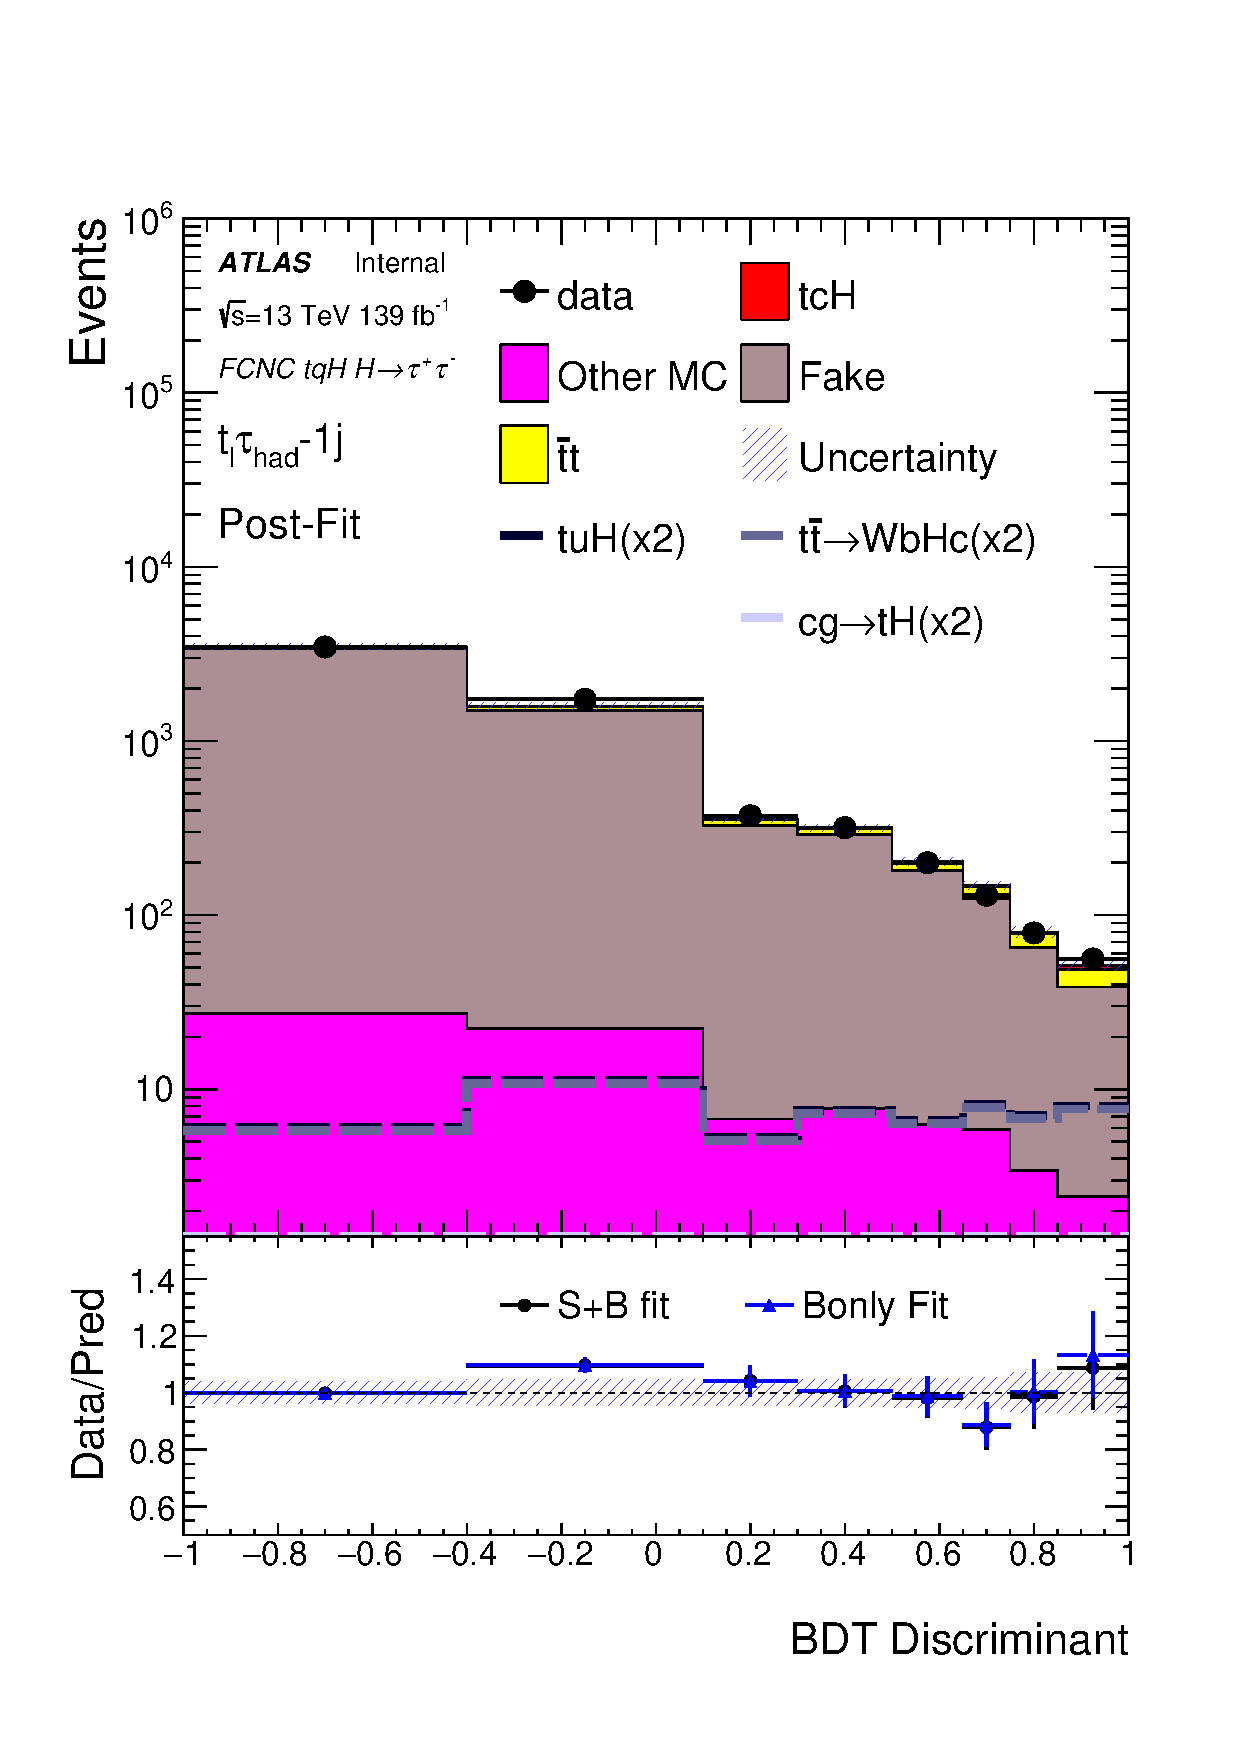
\includegraphics[width=0.29\textwidth]{figures/tcH_reg1l1tau1b1j_ss.pdf}&
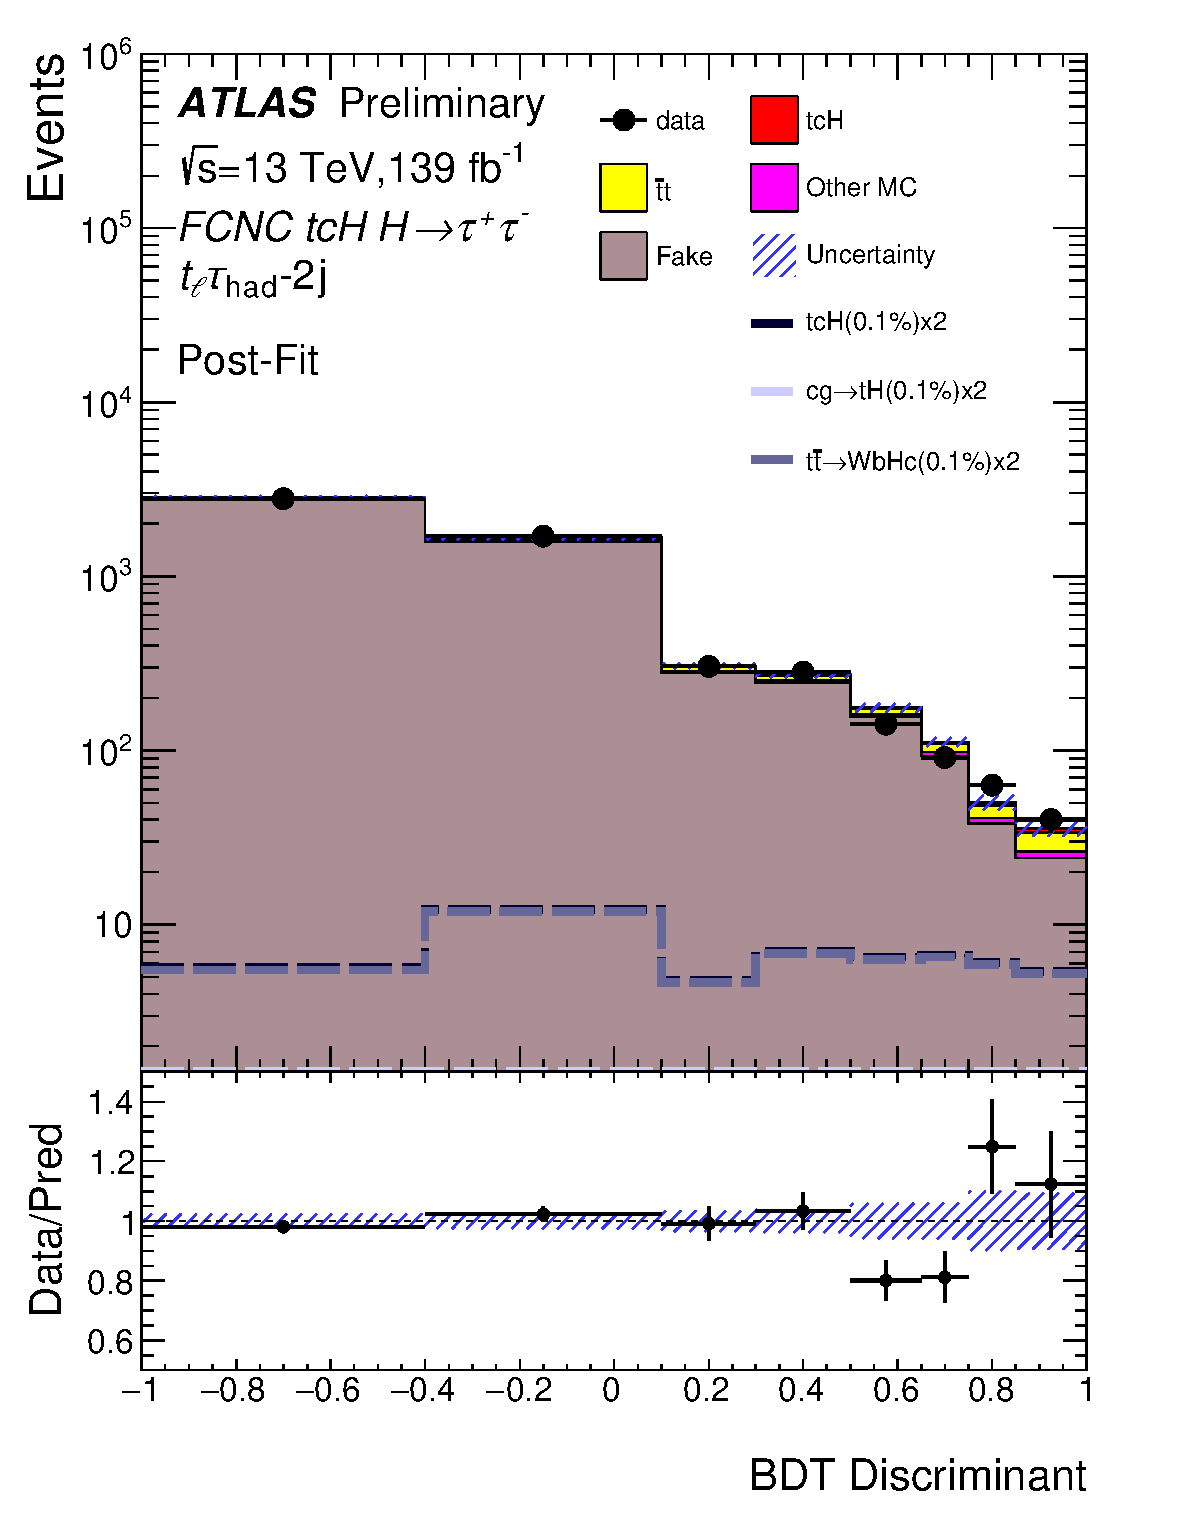
\includegraphics[width=0.29\textwidth]{figures/tcH_reg1l1tau1b2j_ss.pdf}\\
%(a1) BDT in $t_{\ell}\thadhad$ & (a2) BDT in  $t_{\ell}\tauhad$-1j& (a3) BDT in $t_{\ell}\tauhad$-2j\\
(a)  & (b) & (c) \\
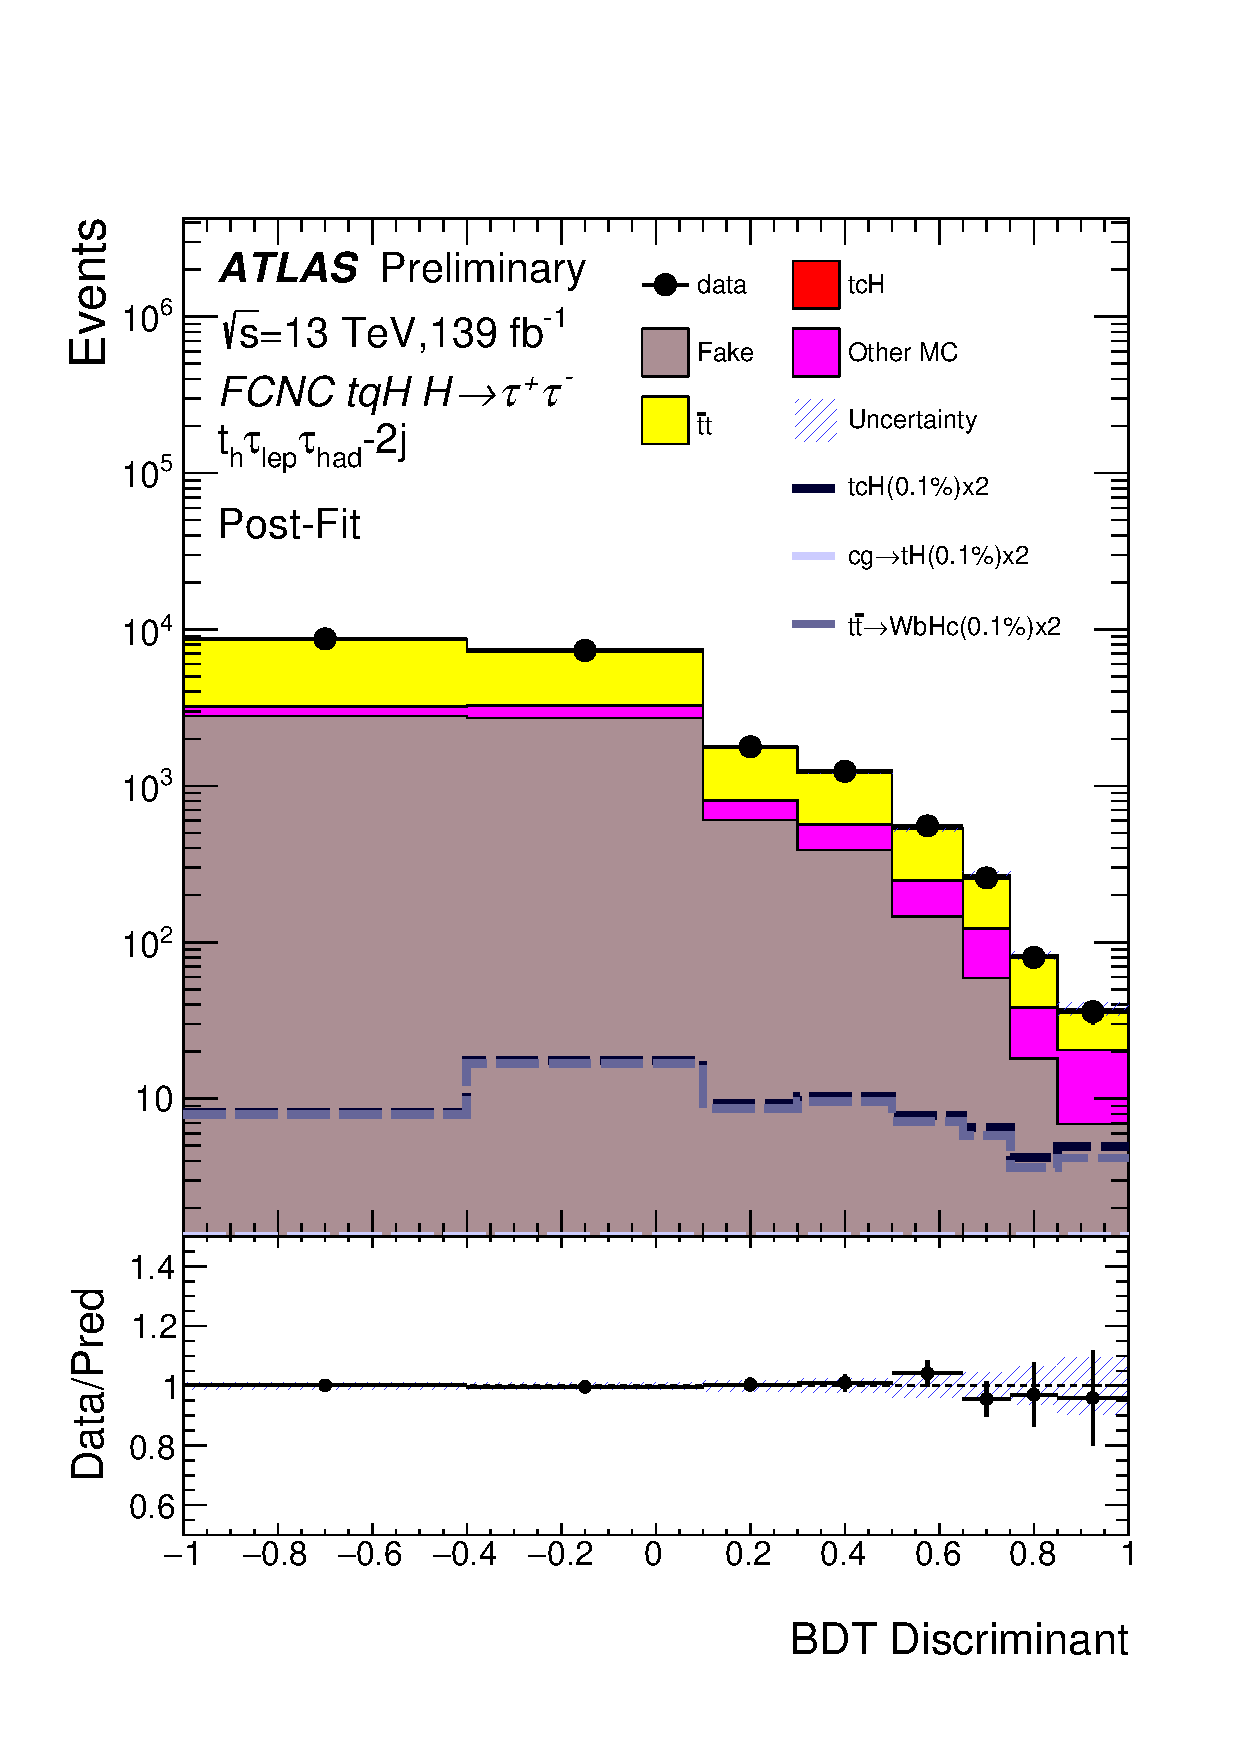
\includegraphics[width=0.29\textwidth]{figures/tcH_reg1l1tau1b2j_os.pdf}&
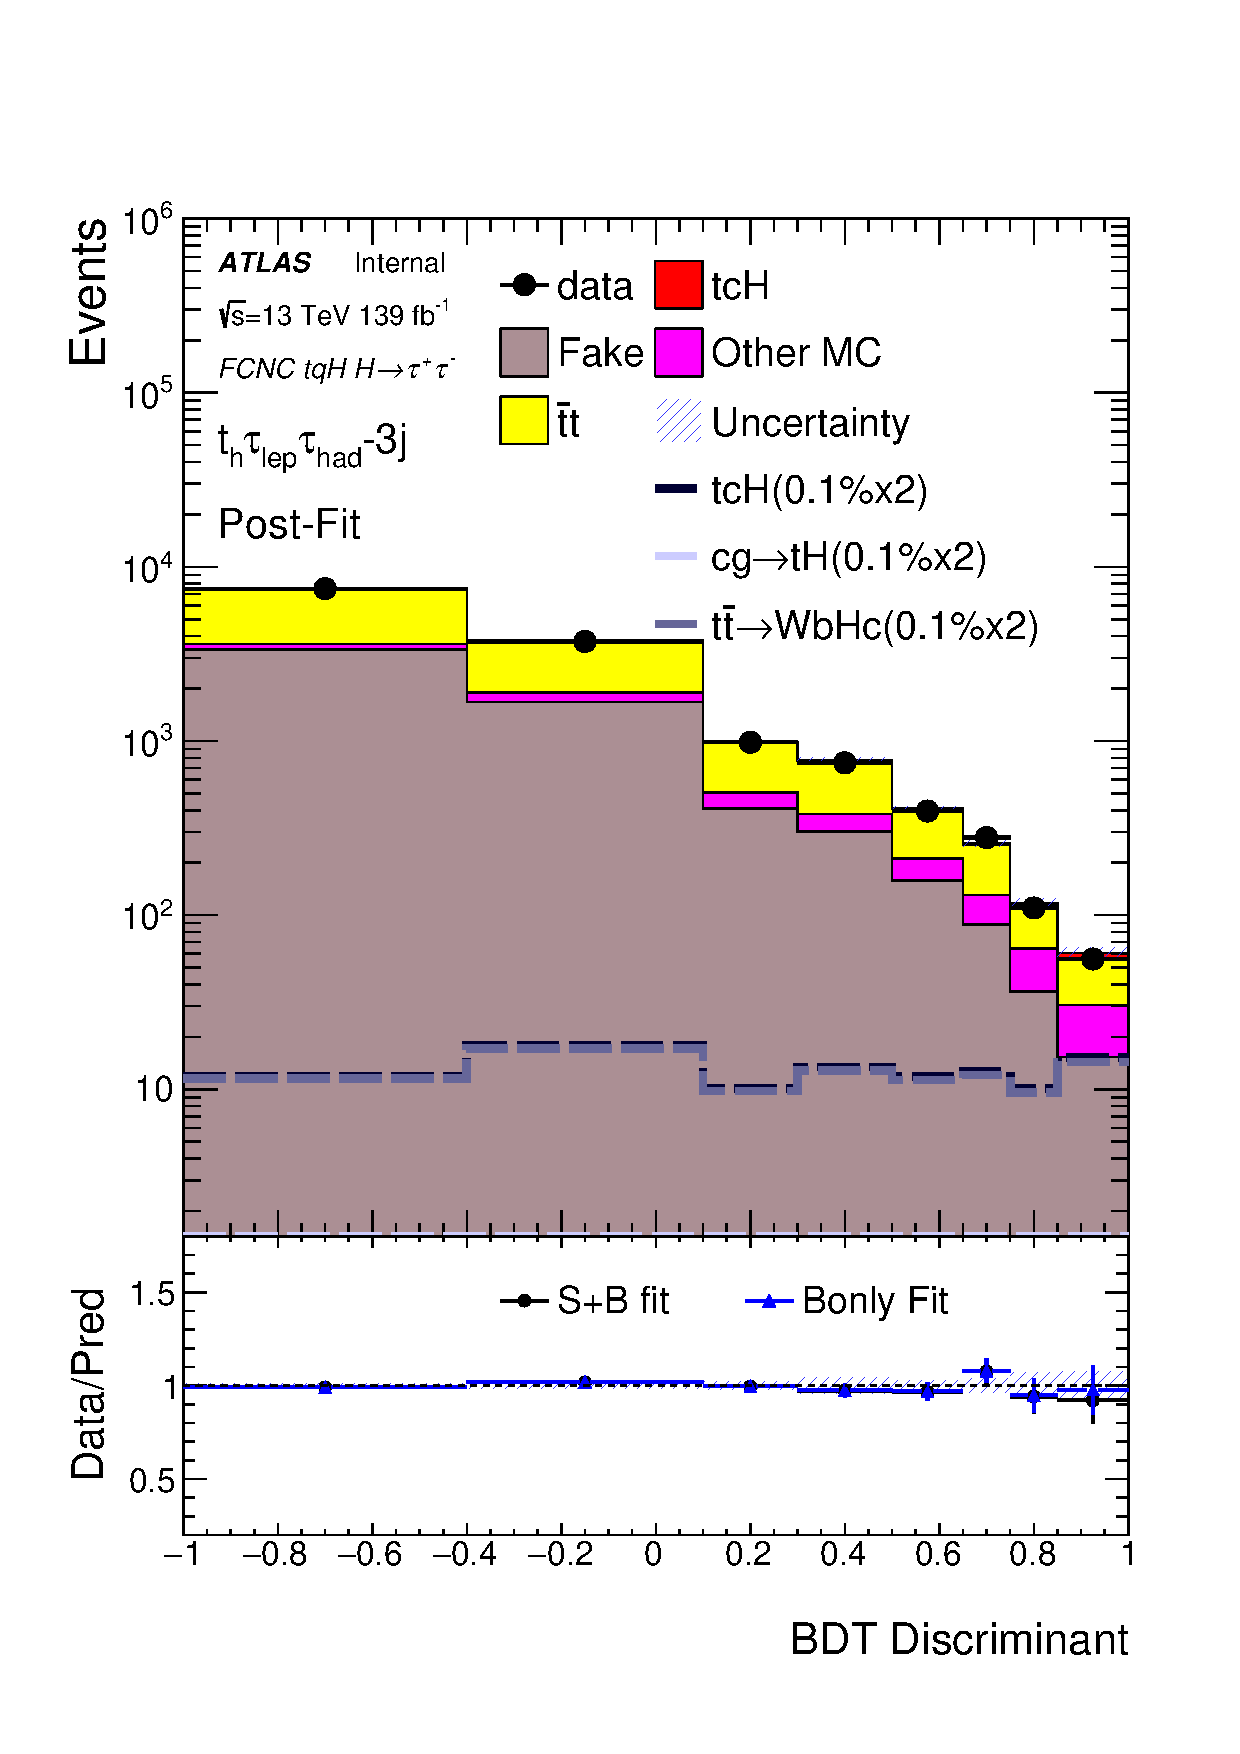
\includegraphics[width=0.29\textwidth]{figures/tcH_reg1l1tau1b3j_os.pdf}&
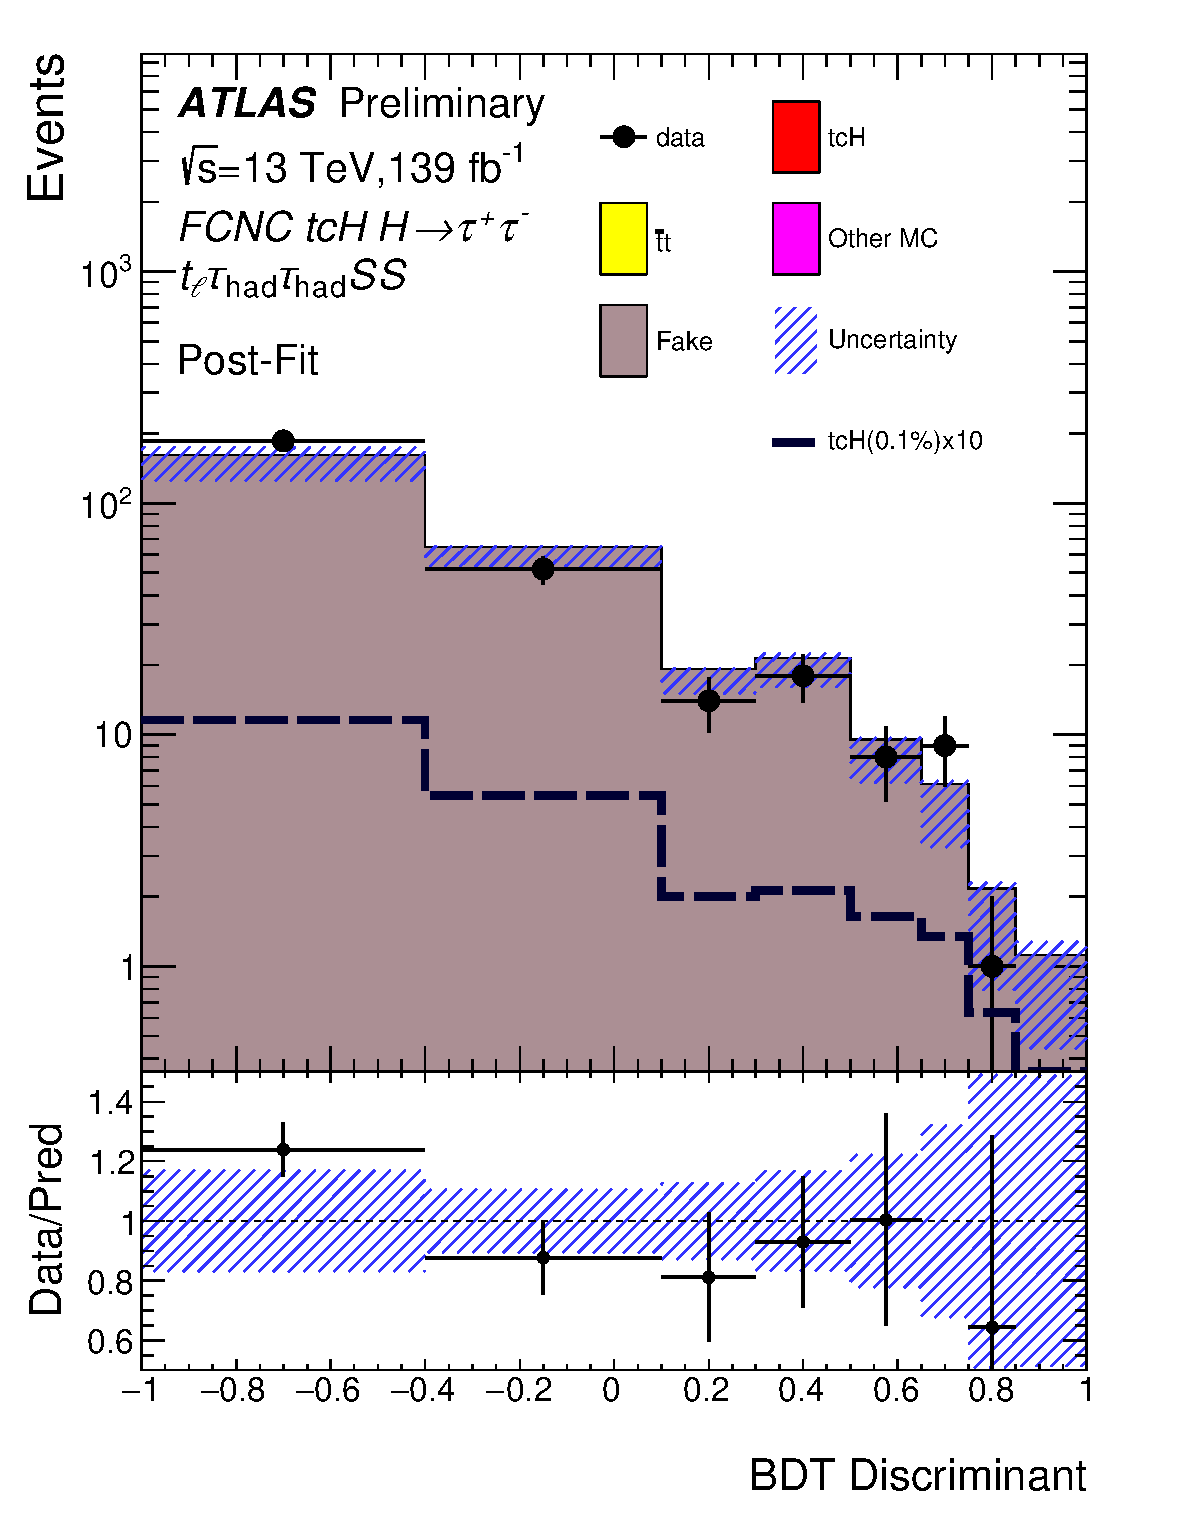
\includegraphics[width=0.29\textwidth]{figures/tcH_reg1l2tau1bnj_ss.pdf}\\
%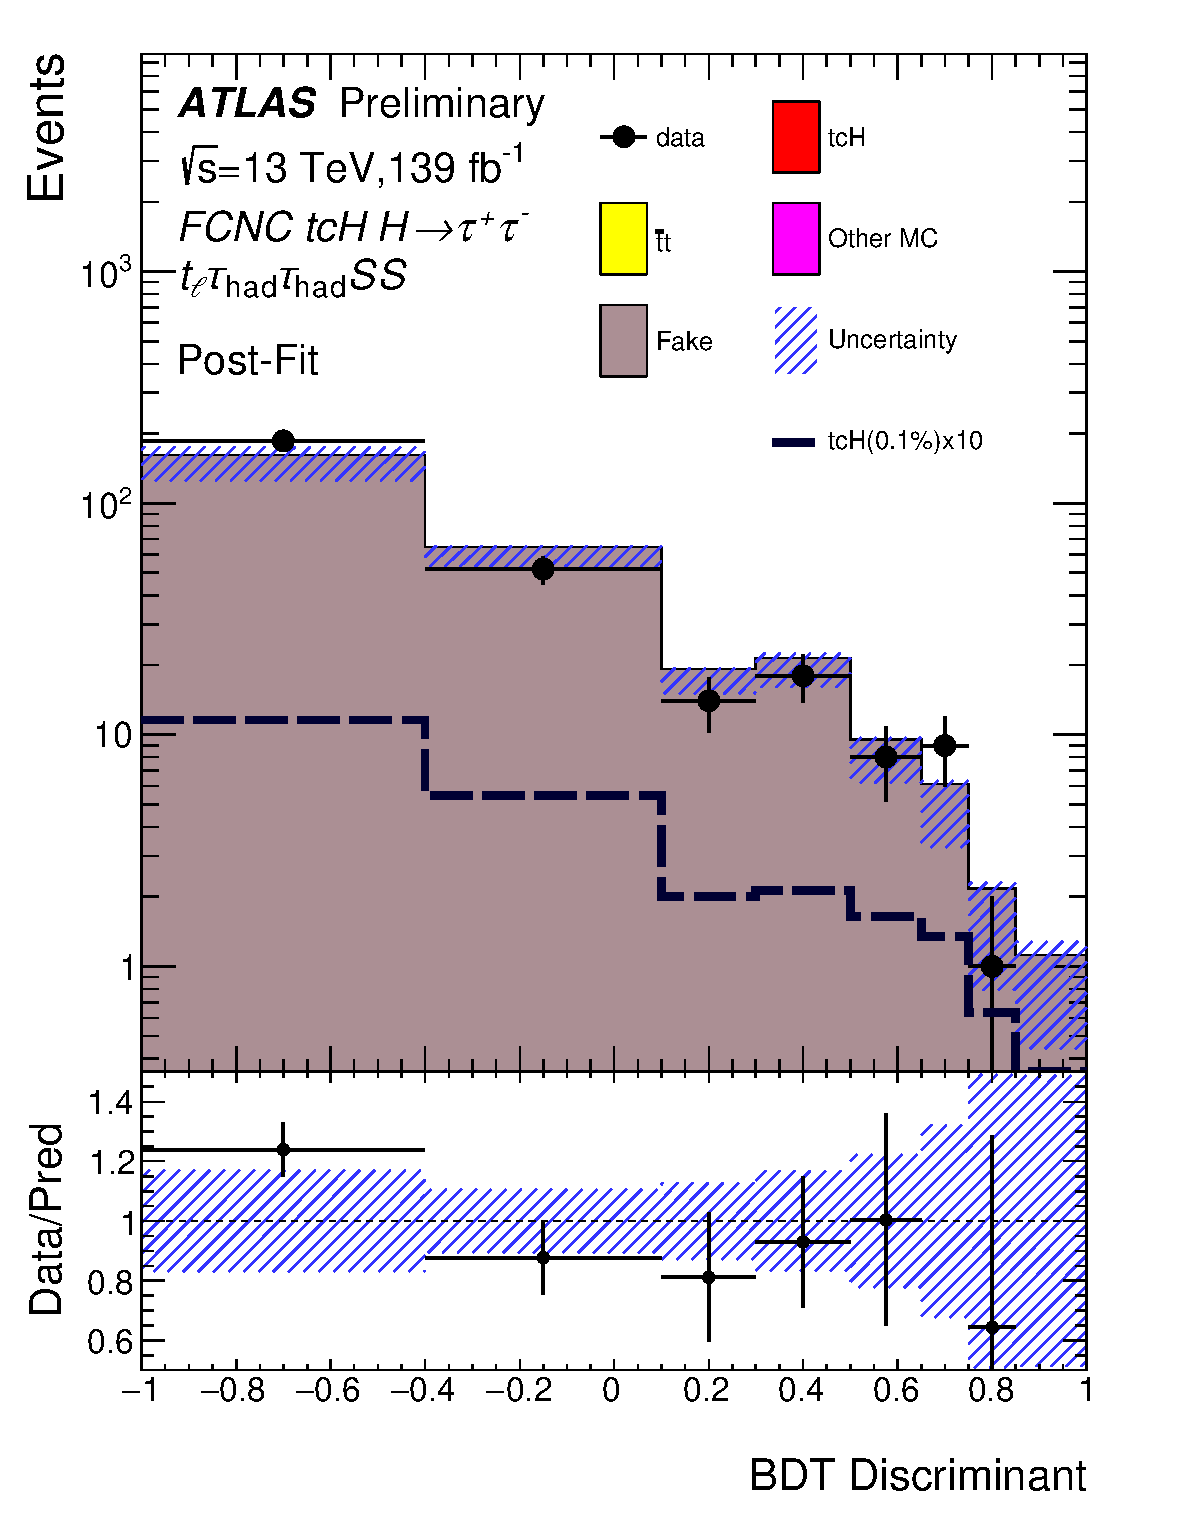
\includegraphics[width=0.3\textwidth]{figures/tcH_reg1l2tau1bnj_ss.pdf}\\
%(b1) BDT in $t_h\tlhad$-2j & (b2) BDT in  $t_h\tlhad$-3j & (b3) BDT in $t_h\thadhad$-2j \\
(d) & (e)  & (f) \\
%(d) & (e)\\
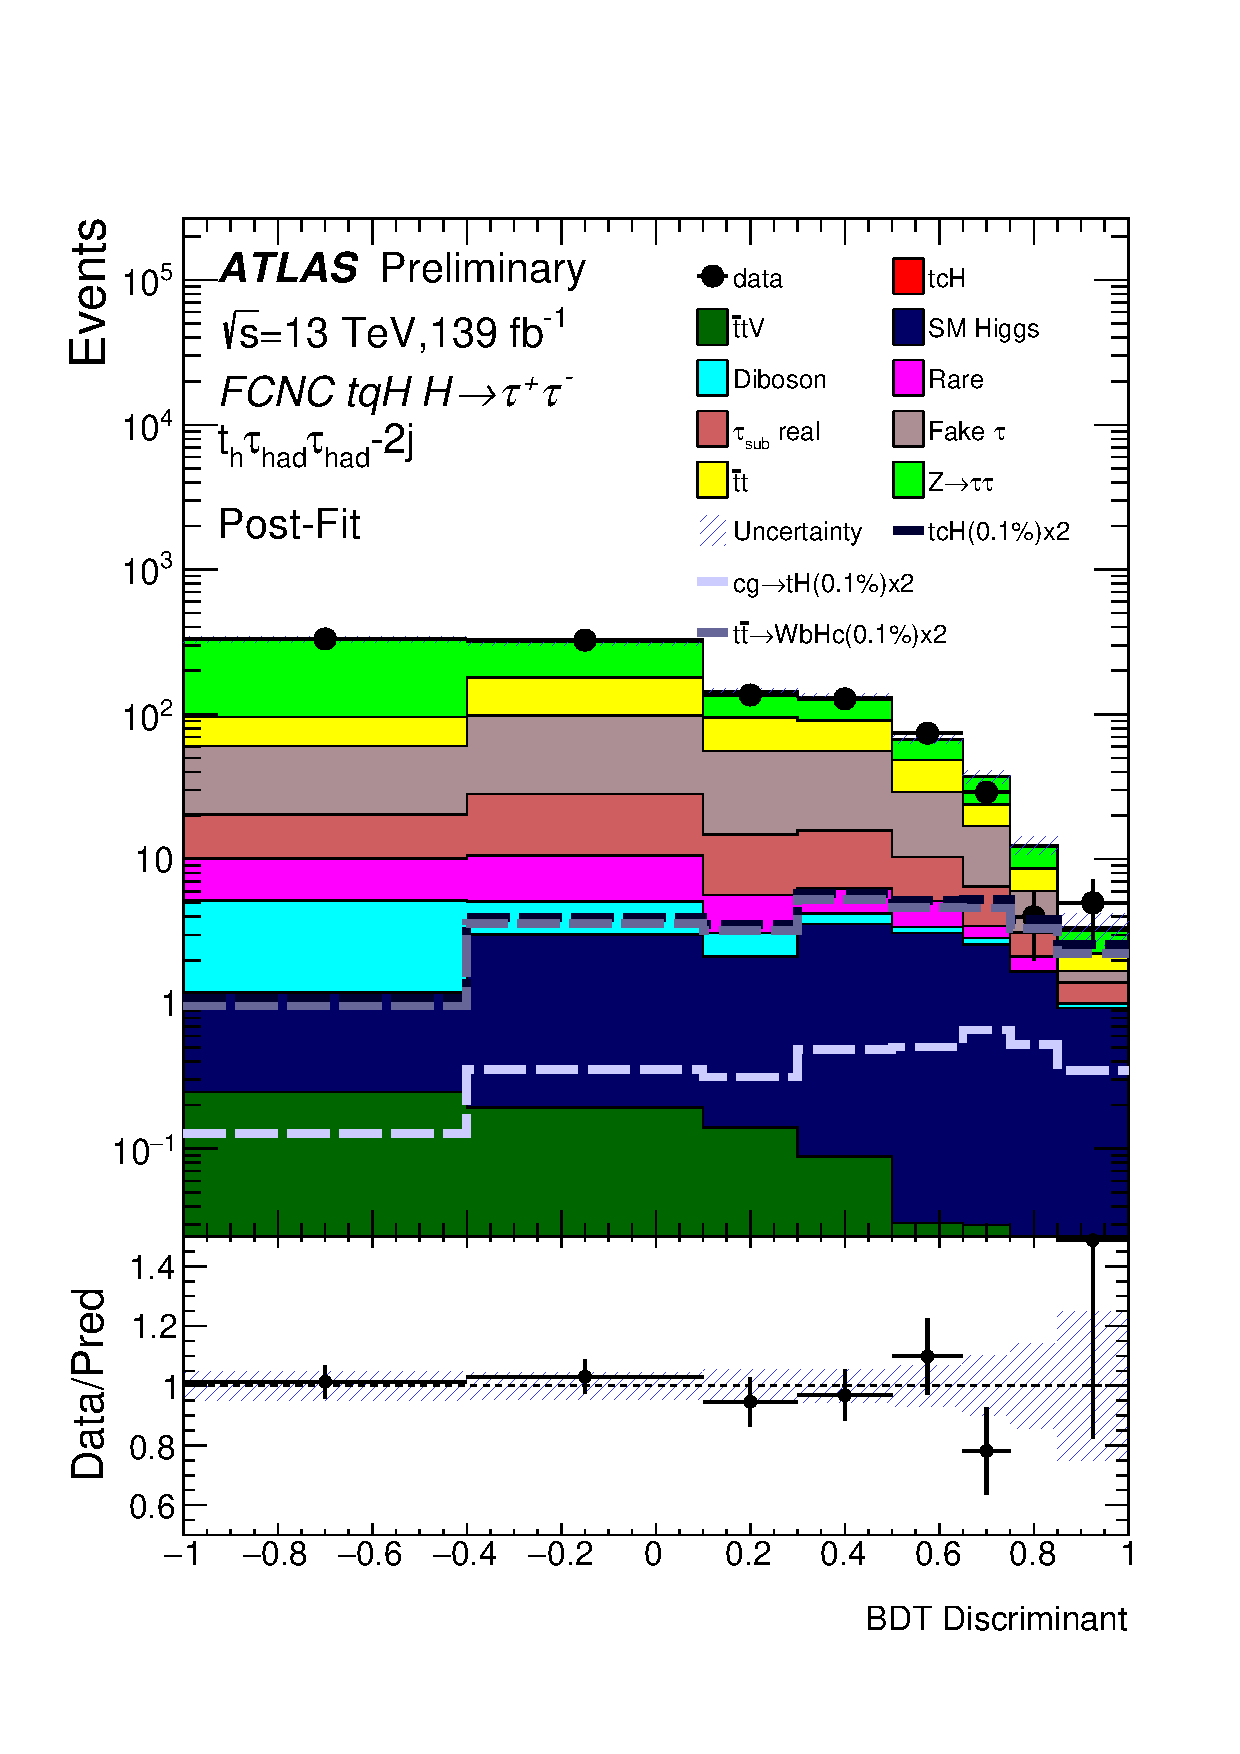
\includegraphics[width=0.29\textwidth]{figures/tcH_reg2mtau1b2jos.pdf}&
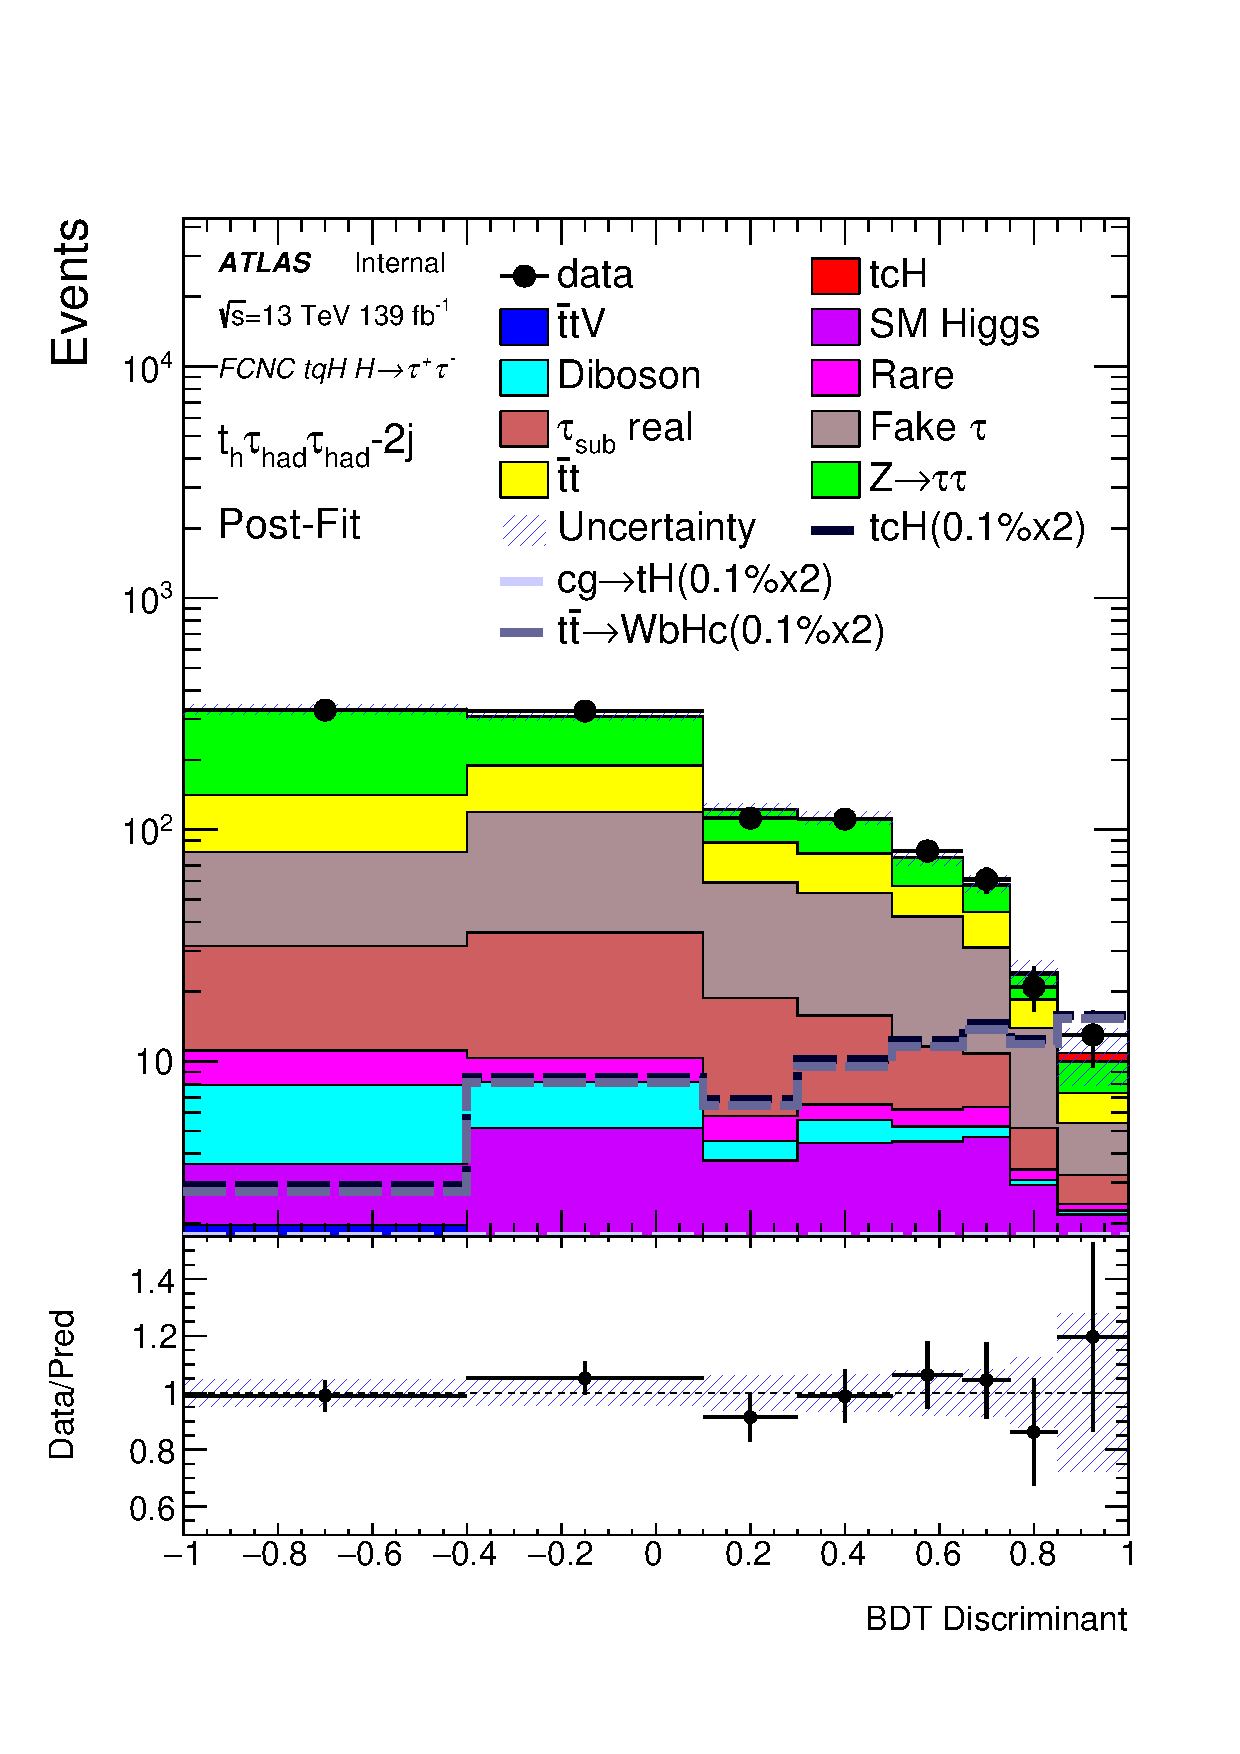
\includegraphics[width=0.29\textwidth]{figures/tcH_reg2mtau1b3jos.pdf}&
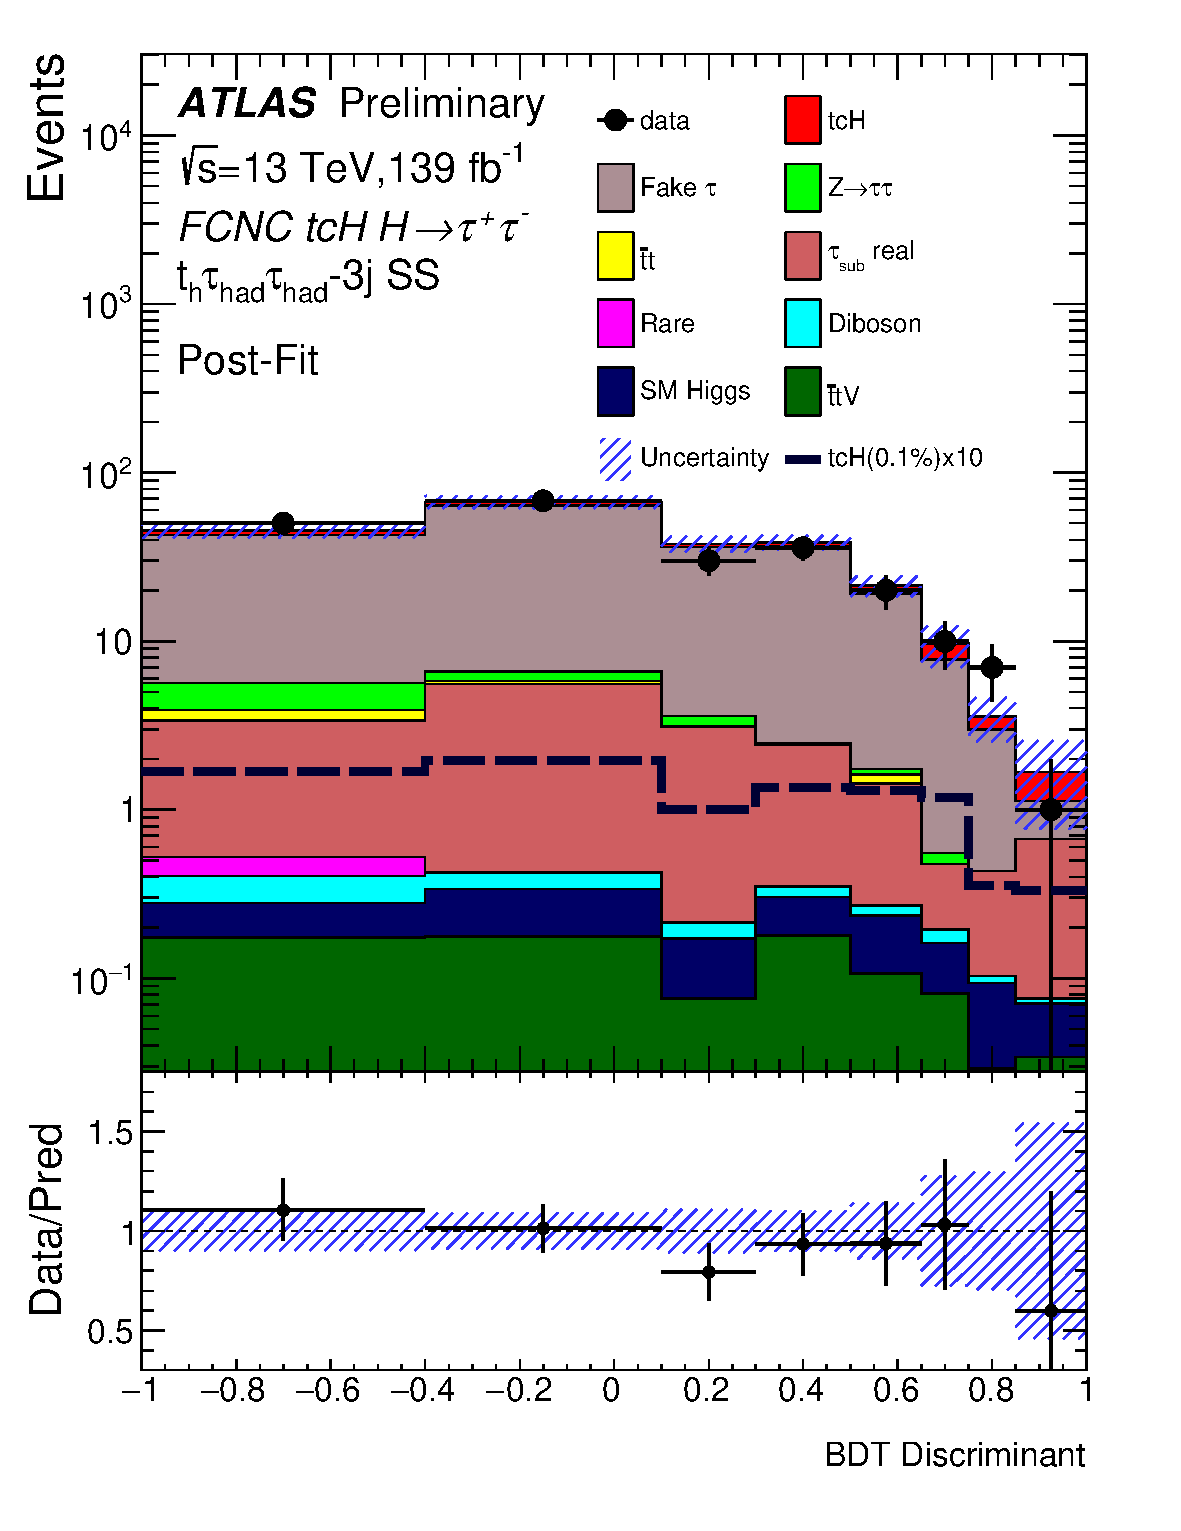
\includegraphics[width=0.29\textwidth]{figures/tcH_reg2mtau1b3jss.pdf}\\
%(c1) BDT in$t_h\thadhad$-3j\\
(g) & (h)  & (i) \\
%(f) & (g)  &  \\
\end{tabular}
\caption{ BDT output distributions obtained from a signal+background fit to the data for the $tcH$ search: 
%$t_{\ell}\thadhad$ (a),  $t_{\ell}\tauhad$-1j (b),  $t_{\ell}\tauhad$-2j (c), $t_h\tlhad$-2j (d), $t_h\tlhad$-3j (e), $t_{\ell}\thadhad$ SS (f), $t_h\thadhad$-2j (g), and $t_h\thadhad$-3j (h), where $t_{\ell}\thadhad$ SS is used for the background validation.
(a) $t_{\ell}\thadhad$, (b) $t_{\ell}\tauhad$-1j,  (c) $t_{\ell}\tauhad$-2j, (d) $t_h\tlhad$-2j, (e) $t_h\tlhad$-3j, (f) $t_{\ell}\thadhad$-SS, (g) $t_h\thadhad$-2j, (h) $t_h\thadhad$-3j and (i) $t_h\thadhad$-3j SS. 
The total statistical and systematic
uncertainty is indicated by the hatched band. The signal shapes of $tt(cH)$, $tH$, and their sum are also shown using a normalisation of $2 \times\BR(t\to cH)$ of 0.1\%.
}
\label{fig:asimov_postfitbdtHc}
\end{figure}

\begin{table}[htbp]
\caption{
  Predicted and observed yields in each of the analysis regions considered. The background prediction is shown after a background-only fit is applied to the data.
  Also shown are the expected signals for $\Hc$ and
  $\Hu$ assuming $\BR(t\to cH)=0.1\%$ and $\BR(t\to uH)=0.1\%$ respectively. The contributions with real $\had$ candidates from $\ttbar$ and  $Z\to \ell^+\ell^-$ ($\ell = e, \mu$),
  diboson, $\ttbar V$, $\ttbar H$, single-top-quark, and other small backgrounds are combined into a single background source referred to as `Other MC' in the leptonic channels,
  whereas single-top-quark and the small contributions are combined into `Rare' in the hadronic channels.
  The quoted uncertainties are the sum in quadrature of the statistical and systematic uncertainties of the yields.}
\small
\centering

\begin{tabular}{cccccc} \toprule\toprule
 & $t_\ell\tauhad$-1j & $t_\ell\tauhad$-2j & $t_h\tlhad$-3j &$t_h\tlhad$-2j  & $t_\ell\thadhad$ \\\midrule
  Double Fake            & $--       $  & $--       $  & $--       $  &  $--       $  & ~~$73 \pm 24    $ \\ 
  $\bar{t}tV$            & ~~$9.3 \pm 1.2 $  & $22.6 \pm 2.8$  & $23.5 \pm 3.0$  &  $13.7 \pm 1.7$  & ~~$2.57 \pm 0.35$ \\ 
  SM Higgs               & ~~$5.8 \pm 0.8 $  & $13.7 \pm 1.7$  & $32.8 \pm 3.5$  &  $13.5 \pm 2.5$  & $16.7 \pm 1.9 $ \\ 
  Diboson                & $32.6 \pm 3.4$  & $19.9 \pm 2.1$  & $36 \pm 4    $  &  $46 \pm 5    $  & $13.2 \pm 1.4 $ \\ 
  Other MC               & $35.6 \pm 3.1$  & $15.9 \pm 1.7$  & $226 \pm 21  $  &  $620 \pm 40  $  & ~~$6.7 \pm 0.6  $  \\ 
  $Z\rightarrow\tau\tau$ & ~~$0 \pm 6     $  & ~~$9.1 \pm 2.2 $  & $500 \pm 60  $  &  $880 \pm 90  $  & ~~$2.1 \pm 0.7  $ \\ 
  Lep.\ Fake               & $212 \pm 30  $  & ~~$80 \pm 10   $  & $292 \pm 26  $  &  $490 \pm 70  $  & ~~$0.9 \pm 0.4  $ \\ 
  QCD Fake               & ~~$670 \pm 200 $  & $310 \pm 90  $  & $180 \pm 70  $  &  ~~$330 \pm 110 $  & $--        $  \\ 
  $b$ Fake                 & ~~$960 \pm 140 $  & $1250 \pm 230$  & ~~$710 \pm 140 $  &  ~~$710 \pm 130 $  & ~~$82 \pm 13    $ \\ 
  $W$-jet Fake             & ~~$970 \pm 200 $  & $1090 \pm 240$  & $3300 \pm 500$  &  $3800 \pm 600$  & ~~$5.5 \pm 1.8  $ \\ 
  Other Fake             & $3020 \pm 260$  & $2470 \pm 160$  & $1420 \pm 220$  &  $1320 \pm 320$  & $129 \pm 14   $ \\ 
  $\bar{t}t$             & $281 \pm 14  $  & $195 \pm 24  $  & $7100 \pm 400$  &  $11800 \pm 500$~~ & ~~$7.7 \pm 2.7  $ \\ \midrule
  Total background       & $6200 \pm 170$  & $5480 \pm 100$  & $13820 \pm 140$~~ &  $20000 \pm 170$~~ & $339 \pm 27   $ \\  \midrule
  $tcH$                    & $30 \pm 5    $  & $27 \pm 4    $  & $51 \pm 8    $  &  $34 \pm 6    $  & $36 \pm 5     $ \\
  $tuH$                    & $36 \pm 8    $  & $32 \pm 5    $  & ~~$63 \pm 10   $  &  $45 \pm 7    $  & $48 \pm 7     $ \\ \midrule
  Data                   & $6353        $  & $5410        $  & $13804       $  &  $20000       $  & $351          $ \\ 
\bottomrule\bottomrule
\end{tabular}\\




\begin{tabular}{ccc} \toprule\toprule
& $t_{h}\thadhad$-2j & $t_{h}\thadhad$-3j\\\midrule
  $t\bar{t}V$              & ~~$0.7 \pm 0.4 $ & ~~$5.5 \pm 1.0 $  \\
  Diboson                  & ~~$8.4 \pm 1.6 $ & $10.8 \pm 1.5$  \\
  Rare                     & $17.9 \pm 3.1$ & $10.2 \pm 2.6$  \\ 
  SM Higgs                 & $17.4 \pm 2.5$ & $25.9 \pm 3.1$  \\ 
  only $\tau_\text{sub}$ real   & ~~$56 \pm 30   $ & ~~$80 \pm 50   $  \\  
  $t\bar{t}$               & $221 \pm 28  $ & $220 \pm 40  $  \\
  Fake $\tau$              & $220 \pm 70  $ & $270 \pm 70  $  \\  
  $Z\rightarrow\tau\tau$   & $490 \pm 50  $ & $420 \pm 50  $  \\ \midrule
  Total background         & $1040 \pm 35 $~~ & $1040 \pm 40 $~~  \\ \midrule
  $tcH$                      & $15.6 \pm 2.5$ & $42 \pm 8    $  \\ 
  $tuH$                      & $23 \pm 4    $ & ~~$52 \pm 10   $  \\ \midrule
  Data                     & $1033       $& $1052 $       \\
\bottomrule\bottomrule
\end{tabular}
\label{tab:HtautauPostfitYieldsUnblind}
\end{table}



%Comparison between the data and prediction for the BDT discriminant distribution in the
%$\lephad$ channel, before and after the fit to data  (``Pre-Fit'' and ``Post-Fit'', respectively) under the signal-plus-background hypothesis.
%Shown are the ($\lephad$, 3j) region (a) pre-fit and (c) post-fit, and the ($\lephad$, $\geq$4j) region (b) pre-fit and (d) post-fit.
%The contributions with real $\had$ candidates from $\ttbar$,  $\ttbar V$, $\ttbar H$, and single-top-quark backgrounds are combined into
%a single background source referred to as ``Top (real $\had$)'', whereas the small contributions from 
%$Z\to \ell^+\ell^-$ ($\ell = e, \mu$) and diboson backgrounds are combined into ``Other''. 
%In the pre-fit figures the expected $\Hc$ signal (solid red) corresponding to $\BR(t\to Hc)=1\%$ is also shown,
%added to the background prediction. In the post-fit figures, the $\Hc$ signal is normalised using the best-fit branching ratio, 
%$\BR(t\to Hc)=(-4.4^{+9.9}_{-8.5})\times 10^{-4}$.
%The bottom panels display the ratios of data to either the SM background prediction before the fit (``Bkg'')  or the total signal-plus-background
%prediction after the fit (``Pred''). 
%The hashed area represents the total uncertainty of the background. 
%In the case of the pre-fit background uncertainty, the normalisation uncertainty of the fake $\had$ background is not included.
%The results are given in terms of exclusion limits despite a small excess of data events above the background expectation is found.
Upper limits on $\BR(t\to cH)$ and $\BR(t\to uH)$ are derived using the CL$_{\textrm{s}}$ method~\cite{Junk:1999kv,Read:2002hq}, and  
the observed (expected) 95\% CL limits are 
$\BR(t\to cH)<9.4 \times 10^{-4}\,(4.8^{+2.2}_{-1.4}\times10^{-4})$, assuming $\BR(t\to uH)=0$, and $\BR(t\to uH)<6.9 \times 10^{-4}\,(3.5^{+1.5}_{-1.0}\times10^{-4})$, assuming $\BR(t\to cH)=0$.
These results are dominated by the leptonic channels, whose sensitivity is a factor of two better than that of the hadronic channels.
The expected sensitivity is a factor of five better than that of the previous ATLAS search, which was based on 36 fb$^{-1}$ of data and used $H\to \tau\tau$ decays~\cite{fcnc36}.
A factor of~2 improvement in sensitivity comes from the larger dataset, and a further factor of~2.5 comes from including
additional leptonic channels, $tH$ production, and improved techniques.

%The best-fit branching ratio obtained is $\BR(t\to Hc)=[xxx^{+yy}_{-yy}\,(\mathrm{stat})^{+zz}_{-zz}\,(\mathrm{syst})] \times 10^{-4}$, assuming $\BR(t\to Hu)=0$. 
%The best-fit normalisation factors for the fake $\had$ background are: $0.82 \pm 0.23$ in the ($\lephad$, 3j) region, $0.84^{+0.25}_{-0.28}$ in the ($\lephad$, $\geq$4j) region,
%$0.94^{+0.18}_{-0.17}$ in the ($\hadhad$, 3j) region, and $0.90 \pm 0.26$ in the ($\hadhad$, $\geq$4j) region.
%A similar fit is performed for the $tuH$ search, yielding $\BR(t\to Hu)=[xxx^{+yy}_{-yy}\,(\mathrm{stat})^{+zz}_{-zz}\,(\mathrm{syst})] \times 10^{-4}$,
%assuming $\BR(t\to Hc)=0$.
%The obtained normalisation factors for the fake $\had$ background agree within 1\% with those obtained by the $\Hc$ search.
In both cases, the results are dominated by the statistical uncertainty.
The main contributions to the total systematic uncertainty arise from  the size of the MC samples,
the uncertainties in the $\thad$ identification efficiency,
%measured $H\to \tautau$ branching ratio,
the renormalisation and factorisation scales, the $b$-tagging efficiency, the choice of parton shower and hadronisation schemes for $t\bar t$ modelling, and
the fake-$\had$ background estimation in the hadronic channels. Their absolute impacts on the signal strength are summarised in Table~\ref{tab:had_sys_impact}.
%the fake $\had$ background estimation in the hadronic channels and the uncertainty associated
%with the different responses to quark-initiated and gluon-initiated jets. 
%o significant excess of data events above the background expectation is found, 
%nd observed (expected) 95\% CL limits are set on $\BR(t\to Hc)$ and $\BR(t\to Hu)$:
%\BR(t\to Hc)<xxx \times 10^{-3}\,(yyy \times 10^{-3})$ and $\BR(t\to Hu)<xxx \times 10^{-3}\,(yyy \times 10^{-3})$.
%hese results are dominated by the leptonic channels, which has a sensitivity a factor of two better than that of the hadronic channels.
%\begin{figure*}[t!]
%\begin{center}
%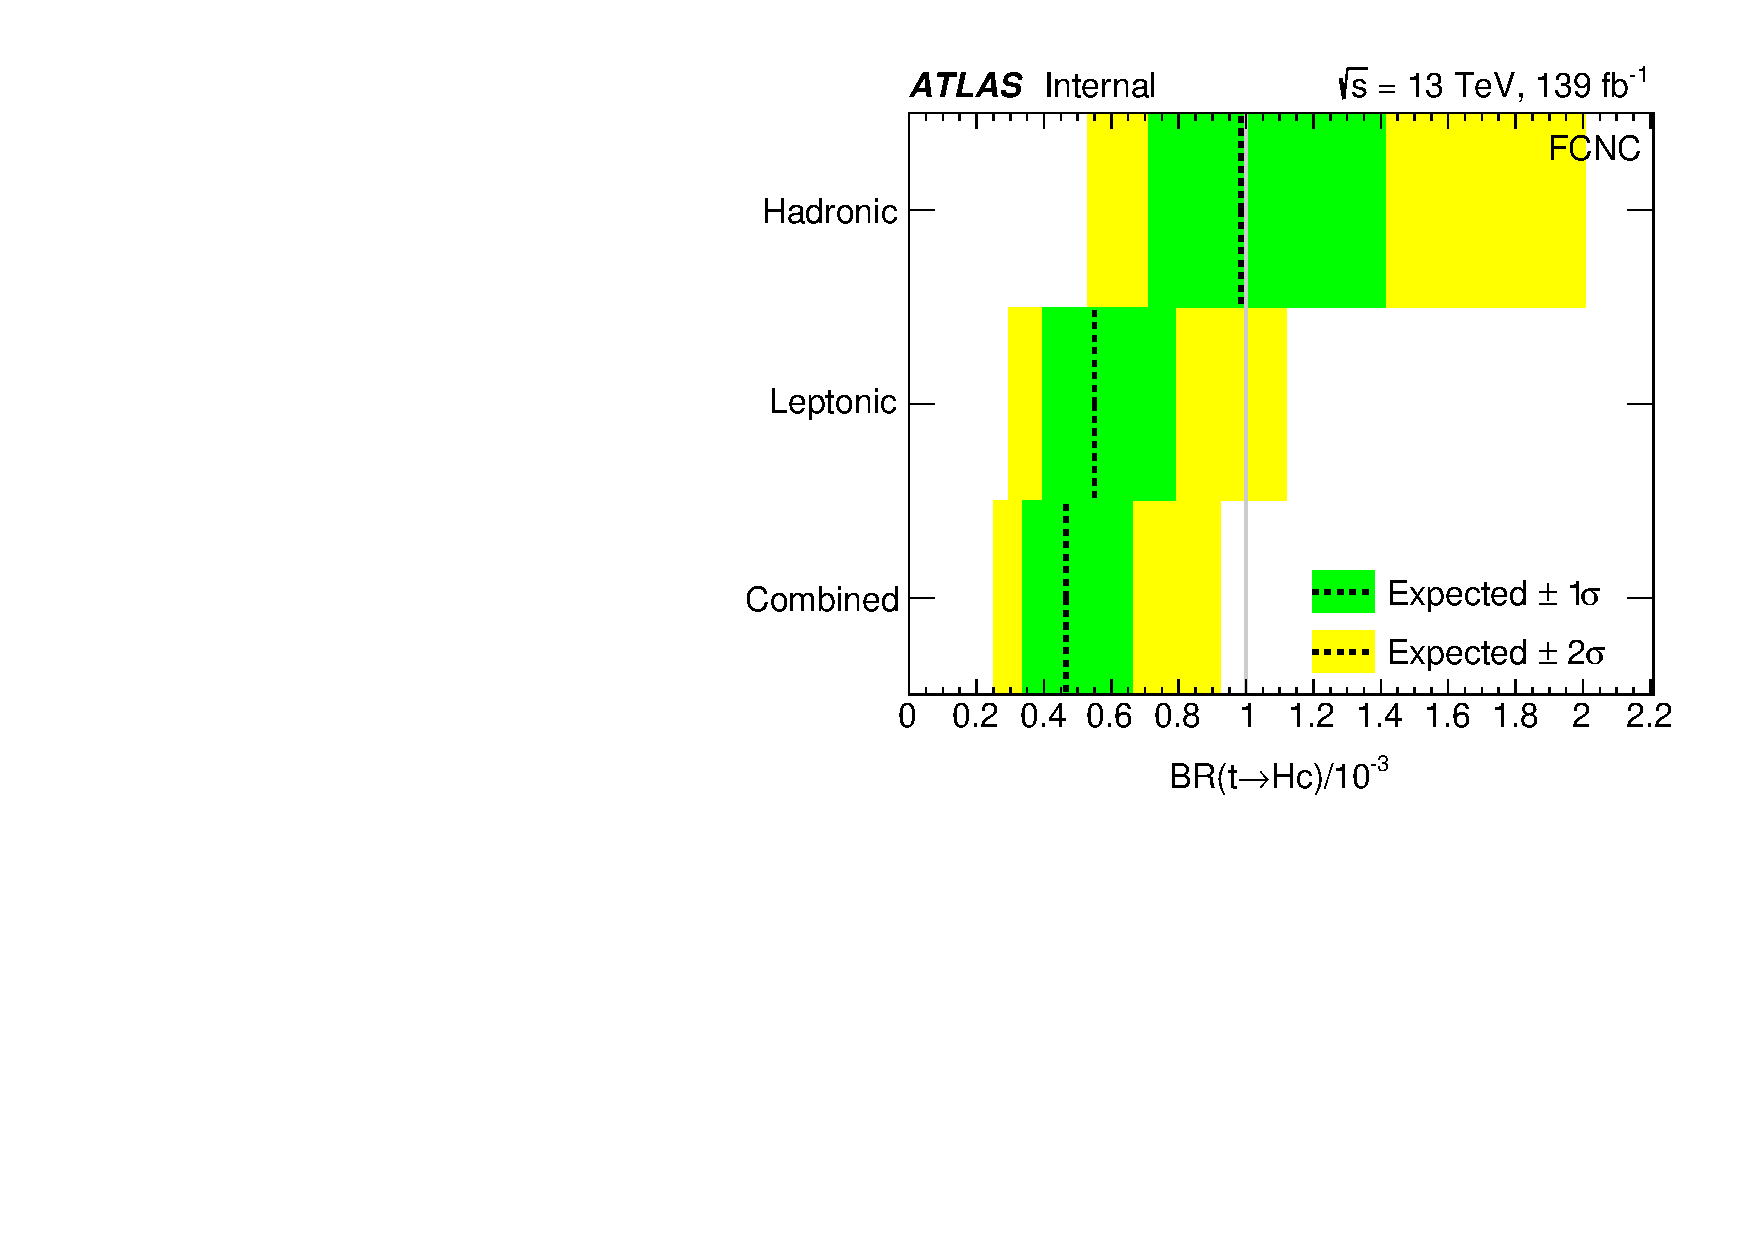
\includegraphics[width=0.7\textwidth]{\FCNCFigures/tcH_combined_Limit.pdf}
%\caption{\small {Summary of the best-fit $\BR(t\to Hc)$ for the individual channels as well as their combination,
%assuming $\BR(t\to Hu)=0$. (TBD: updated with best fit plots.)}}
%\label{fig:summary_printnum_hc} 
%\end{center}
%\end{figure*}
%%%%%%%%%%%%%%
%%%%%%%%%%%%%%
%\begin{figure*}[h!]
%\begin{center}
%\includegraphics[width=0.7\textwidth]{\FCNCFigures/tuH_combined_Limit.pdf}
%\caption{\small {Summary of the best-fit $\BR(t\to Hu)$ for the individual channels as well as their combination,
%assuming $\BR(t\to Hc)=0$. (TBD: updated with best fit plots.)}}
%\label{fig:summary_printnum_hu} 
%\end{center}
%\end{figure*}
%%%%%%%%%%%%%%
%The first set of combined results is obtained for each branching ratio separately, setting the other branching ratio to zero.
%The best-fit combined branching ratios are $\BR(t\to Hc)=[3.0^{+3.0}_{-2.7}\,(\mathrm{stat})^{+2.6}_{-2.1}\,(\mathrm{syst})] \times 10^{-4}$ and 
%$\BR(t\to Hu)=[4.2^{+3.2}_{-2.9}\,(\mathrm{stat})^{+2.6}_{-2.1}\,(\mathrm{syst})] \times 10^{-4}$.  
%%The difference between the central values of $\BR(t\to Hc)$ and $\BR(t\to Hu)$ originates from the ability of the $H \to b\bar{b}$ search to 
%%probe both decay modes separately.
%A comparison of the best-fit branching ratios for the individual searches and their combination is shown in Figure~\ref{fig:summary_printnum_hc} 
%for $\BR(t\to Hc)$ and Figure~\ref{fig:summary_printnum_hu} for $\BR(t\to Hu)$.
%The observed (expected) 95\% CL combined upper limits on the branching ratios are 
%$\BR(t\to Hc)<1.1 \times 10^{-3}\,(8.3 \times 10^{-4})$ and $\BR(t\to Hu)<1.2 \times 10^{-3}\,(8.3 \times 10^{-4})$.
A summary of the upper limits, significance and best-fit values of the branching ratios obtained by the individual searches, as well as their combination, is given  
%%in Table~\ref{tab:limits_summary}, as is displayed in Figures~\ref{fig:limits_combo_1D_hc} and~\ref{fig:limits_combo_1D_hu}.
in Table~\ref{tab:limits_summary} and in Figures~\ref{fig:limits_combo_1D_hc}(a) and~\ref{fig:limits_combo_1D_hc}(b).

\begin{table}[h!]
  \caption{Absolute uncertainties in $\BR(t\to qH)$ ($q=u,c$) obtained from the combined fit to the data. The uncertainties are symmetrised
    and grouped into the categories described in Section~\ref{sec:systematics}.}
\label{tab:had_sys_impact}
% \begin{center}
%   \begin{tabular}{%
%       @{}l%
%       S
%       S
%       @{}
%     }
%     \toprule\toprule
%     \multirow{2}{*}{Source of uncertainty}      & \multicolumn{2}{c}{$\Delta\BR$ [$10^{-5}$]} \\
%     & \multicolumn{1}{c}{$t\rightarrow uH$} & \multicolumn{1}{c}{$t\rightarrow cH$} \\\midrule
%     Lepton ID                               & 0.6           &1.0         \\
%     $\met$                                  & 0.7           &0.8         \\
%     Fake lepton  modeling                   & 0.9           &1.1         \\
%     JES and JER                             & 2.4           &3.2         \\
%     Flavour tagging                         & 2.7           &3.7         \\
%     $t\bar{t}$ modeling                     & 2.9           &4.3         \\
%     Other MC modeling                       & 2.1           &2.9         \\
%     Fake $\tau$ modeling                    & 3.2           &4.6         \\
%     Signal modeling including Br($H\to\tau\tau$)            &5.3           &7.0         \\
%     $\tau$ ID                               & 3.3           &4.4         \\
%     Luminosity and Pileup                   & 0.9           &1.3         \\    
%     MC statistics              & 5.1           &7.0         \\\midrule
%     %Other MC modeling                       & 2.1           &2.9         \\
%     %JES and JER                             & 2.4           &3.2         \\
%     %Flavour tagging                         & 2.7           &3.7         \\
%     %$t\bar{t}$ modeling                     & 2.9           &4.3         \\
%     %Fake $\tau$ modeling                    & 3.2           &4.6         \\
%     %$\tau$ ID                               & 3.3           &4.4         \\
%     %Signal modeling including Br($H\to\tau\tau$)       & 5.3           &7.0         \\\midrule
%     Total systematic uncertainty                            & 11.2          &15.5        \\
%     Data statistical uncertainty                           & 14.1          &19.6         \\\midrule
%     Total uncertainties                       & 18            &25        \\
%     %Total systematic  uncertainty            & 11.2          &15.5        \\
%     %Total statistical uncertainty            & 14.1          &19.6         \\\midrule
%     %Total                                    & 18            &25        \\
%     \bottomrule\bottomrule
%   \end{tabular}
% \end{center}
% \end{table}
 \begin{center}
   \begin{tabular}{%
       @{}l%
       S
       S
       @{}
     }
     \toprule\toprule
     \multirow{2}{*}{Source of uncertainty}      & \multicolumn{2}{c}{$\Delta\BR$ [$10^{-5}$]} \\
     & \multicolumn{1}{c}{$t\rightarrow uH$} & \multicolumn{1}{c}{$t\rightarrow cH$} \\\midrule
     Lepton ID                               & 0.6           &0.8         \\
     $\met$                                  & 0.7           &0.7         \\
     Fake-lepton  modelling                   & 1.2           &1.7         \\
     JES and JER                             & 2.5           &3.3         \\
     Flavour tagging                         & 2.7           &3.7         \\
     $t\bar{t}$ modelling                     & 2.6           &3.9         \\
     Other MC modelling                       & 2.1           &3.0         \\
     Fake-$\tau$ modelling                    & 3.3           &4.7         \\
     Signal modelling including $\BR(H\to\tau\tau)$&1.8        &1.5         \\
     $\tau$ ID                               & 3.3           &4.4         \\
     Luminosity and pile-up                   & 1.7           &2.4         \\    
     MC statistics                           & 5.1           &7.1         \\\midrule
     Total systematic uncertainty            & 10.1          &14.1        \\
     Data statistical uncertainty            & 14.9          &19.4        \\\midrule
     Total uncertainties                     & 18            &24          \\
     \bottomrule\bottomrule
   \end{tabular}
 \end{center}
 \end{table}


Upper limits on the branching ratios $\BR(t\to qH)$ ($q=u,\, c$) can be translated into upper limits on the dimension-6 (D6) operator Wilson coefficients ($C^{i3}_{u\phi}$,
$C^{3i}_{u\phi}$) appearing in the effective field theory Lagrangian for the $tqH$ interaction~\cite{fcnc_production_theory}:
%
\begin{equation*}
  \mathcal{L}_{EFT} = \frac{C^{i3}_{u\phi}}{\Lambda^{2}}(\phi^{\dagger}\phi)(\bar{q_{i}}t)\tilde{\phi} + \frac{C^{3i}_{u\phi}}{\Lambda^{2}}(\phi^{\dagger}\phi)(\bar{t}q_{i})\tilde{\phi}
  \label{eq:eq01}
\end{equation*}
%
where the subscript $i=1,\, 2$ represents the generation of the light-quark fields ($q=u,\, c$).
The branching ratio $\BR(t\to qH)$ is estimated as the ratio of its partial width to the SM $t \to Wb$ partial width including next-to-leading-order QCD corrections. The coefficients can be extracted as $C_{q\phi} = \sqrt{1946.6~\BR(t\to qH)}$~\cite{fcnc_production_theory}. The $C_{q\phi}$ coefficient corresponds to the sum in quadrature of the coefficients relative to the two possible chirality combinations of the quark fields,
$C_{q\phi} =\sqrt{(C^{i3}_{q\phi})^2 + (C^{3i}_{q\phi})^2}$~\cite{fcnc_production_theory}. The observed (expected) upper limits on the D6 Wilson coefficients from the combination of the search
results are $C_{c\phi}<1.35\,(0.97)$ and $C_{u\phi}<1.16\,(0.82)$ for a new-physics scale $\Lambda=1$~\TeV. 

%Upper limits on the branching ratios $\BR(t\to Hq)$ ($q=u,c$) can be translated into upper limits on the non-flavour-diagonal Yukawa couplings $\lamHq$ 
%appearing in the Lagrangian~\cite{Harnik:2012pb}:
%\begin{equation*}
%{\cal L}_\mathrm{FCNC} = -\lambda_{t_\mathrm{L} q_\mathrm{R}} \bar{t}_\mathrm{L} q_\mathrm{R} H - \lambda_{q_\mathrm{L} t_\mathrm{R}} \bar{q}_\mathrm{L} t_\mathrm{R} H  + \mathrm{h.c.}
%\end{equation*}
%The branching ratio $\BR(t\to Hq)$ is estimated as the ratio of its partial width~\cite{Zhang:2013xya} to the SM $t \to Wb$ partial width~\cite{Denner:1990ns}, 
%which is assumed to be dominant. Both predicted partial widths include next-to-leading-order QCD corrections.
%Using the expression derived in Ref.~\cite{Aad:2014dya}, the coupling $|\lamHq|$ can be extracted as $| \lamHq | = (1.92 \pm 0.02) \sqrt{\BR(t\to Hq)}$.
%The $\lamHq$ coupling corresponds to the sum in quadrature of the couplings relative to the two possible chirality combinations of the quark fields, 
%$\lamHq \equiv \sqrt{ |\lambda_{t_\mathrm{L} q_\mathrm{R}}|^2 +   |\lambda_{q_\mathrm{L} t_\mathrm{R}}|^2 }$~\cite{Harnik:2012pb}.
%The observed (expected) upper limits on the couplings from the combination of the searches are $|\lamHc|<0.064\,(0.055)$ and $|\lamHu|<0.066\,(0.055)$.

%%%%%%%%%%%%%%%

%%%%% mu benchmark is 0.1%

% \begin{table}[t!]
% \caption{\small{Summary of 95\% CL upper limits on $\BR(t \to cH)$ and $\BR(t \to uH)$, in each case neglecting the other decay mode. }}
% \begin{center}
% \begin{tabular}{lcc}
% \toprule\toprule
%  & \multicolumn{1}{c}{95\% CL upper limits} & \multicolumn{1}{c}{95\% CL upper limits}  \\
%  & \multicolumn{1}{c}{on $\BR(t \to cH)$} & \multicolumn{1}{c}{on $\BR(t \to uH)$} \\
%  &  Observed (Expected) & Observed (Expected)  \\
% \midrule\midrule
% hadronic  & $1.0 \times 10^{-3}$ ($9.8 \times 10^{-4}$) & $7.8 \times 10^{-4}$ ($7.8 \times 10^{-4}$) \\ 
% leptonic  & $1.3 \times 10^{-3}$ ($5.9 \times 10^{-4}$) & $9.2 \times 10^{-4}$ ($4.2 \times 10^{-4}$) \\
% \midrule
% Combination  & $9.9 \times 10^{-4}$ ($5.0 \times 10^{-4}$) & $7.2 \times 10^{-4}$ ($3.6 \times 10^{-4}$) \\
% \bottomrule\bottomrule
% \end{tabular}
% \label{tab:limits_summary}
% \end{center}
% \end{table}
% %%%%%%%%%%%%%%%

%      \begin{table}[t!]
%        \caption{\small{Summary of 95\% CL upper limits on $\BR(t \to cH)$ and $\BR(t \to uH)$, significance and best-fit branching ratio in signal regions with a
%        benchmark branching ratio of $\BR(t \to qH)=0.1\%$}. Expected significance is obtained from Asimov fit with a signal injection corresponding to a branching ratio of 0.1\%. }
%      \begin{center}
%      \resizebox{\textwidth}{!}{
%      \begin{tabular}{lcccccc}
%      \toprule\toprule
%      
%      \multirow{3}{*}{Signal Regions} & \multicolumn{3}{c}{$t\to cH$}                                & \multicolumn{3}{c}{$t\to uH$}  \\
%                                      &  95\% CL upper limits[$10^{-3}$]  & Significance             &  $\BR[10^{-3}]$ &     95\% CL upper limits[$10^{-3}$]  & Significance   &  $\BR%[10^{-      3}]$  \\
%                                      &  \multicolumn{2}{c}{Observed (Expected)}                     &        &     \multicolumn{2}{c}{Observed (Expected)}& \\
%      \midrule
%      $t_h\thadhad$-2j                & $1.85$($2.80^{+1.30}_{-0.78}$)&$-0.96$($0.78$) & $-1.03^{+1.04}_{-1.04}$&$1.10$($1.65^{+0.79}_{-0.46}$)&$-0.90$($1.25$) &$-0.55^{+0.59}_{-0.59%}$ \\
%      $t_h\thadhad$-3j                & $1.18$($1.06^{+0.50}_{-0.30}$)&$0.34$($1.87$)  & $0.16^{+0.47}_{-0.47}$ &$1.00$($0.89^{+0.42}_{-0.25}$)&$0.36$($2.13$)  &$0.14^{+0.40}_{-0.40}%$  \\       \midrule
%      Hadronic Combination            & $1.04$($0.98^{+0.46}_{-0.28}$)&$0.26$ ($1.99$) & $0.11^{+0.43}_{-0.43}$ &$0.78$($0.78^{+0.37}_{-0.22}$)&$0.11$($2.33$)  &$0.04^{+0.34}_{-0.34}%$  \\
%      \midrule
%      $t_l\tauhad$-2j                 &$4.86$($4.32^{+1.89}_{-1.21}$) &$0.40$($0.48$)   &$0.81^{+2.04}_{-2.04}$  & $3.93$($3.55^{+1.56}_{-0.99}$) & $0.34$($0.58$)  &$0.57^{+1.66}_{-%1.66}$      \\
%      $t_l\tauhad$-1j                 &$3.94$($3.67^{+1.66}_{-1.03}$) &$0.24$($0.57$)   &$0.40^{+1.70}_{-1.70}$  & $3.10$($2.87^{+1.29}_{-0.80}$) & $0.24$($0.73$)  &$0.31^{+1.33}_{-%1.33}$      \\
%      $t_h\tlhad$-2j                  &$4.81$($5.85^{+2.90}_{-1.63}$) &$-0.52$($0.39$)  &$-1.36^{+2.56}_{-2.56}$ & $2.56$($3.05^{+1.38}_{-0.85}$) & $-0.48$($0.69$) &$-0.66^{+1.38}_{-%1.38}$      \\
%      $t_h\tlhad$-3j                  &$2.78$($2.79^{+1.36}_{-0.78}$) &$-0.04$($0.76$)  &$-0.04^{+1.26}_{-1.26}$ & $2.07$($2.09^{+0.94}_{-0.58}$) & $-0.05$($0.98$) &$-0.04^{+0.98}_{-%0.98}$      \\
%      $t_l\thadhad$                   &$1.41$($0.63^{+0.29}_{-0.18}$) &$2.64$($3.24$)   &$0.74^{+0.34}_{-0.34}$  & $1.01$($0.45^{+0.21}_{-0.13}$) & $2.64$($4.08$)  &$0.53^{+0.25}_{-%0.25}$      \\ \midrule
%      Leptonic Combination            &$1.29$($0.59^{+0.27}_{-0.17}$) &$2.59$($3.34$)   &$0.68^{+0.32}_{-0.32}$  & $0.92$($0.42^{+0.19}_{-0.12}$) & $2.59$($4.23$)  &$0.48^{+0.23}_{-%0.23}$      \\
%      \midrule
%      Combination                     &$0.99$ ($0.50^{+0.22}_{-0.14}$)&$2.34$($3.69$)   &$0.51^{+0.25}_{-0.25}$ & $0.72$ ($0.36^{+0.17}_{-0.10}$)& $2.31$($4.49$)&$0.37^{+0.18}_{-0.18%}$  \\
%      \bottomrule\bottomrule
%      \end{tabular}
%      }
%      \label{tab:limits_summary}
%      \end{center}
%      \end{table}
%%%%%%%%%%%%%%%


\begin{table}[t!]
  \caption{\small{Summary of 95\% CL upper limits on $\BR(t \to cH)$ and $\BR(t \to uH)$, significance and best-fit branching ratio in the signal regions with a
  benchmark branching ratio of $\BR(t \to qH)=0.1\%$}. The expected significance is obtained from an Asimov fit~\cite{Cowan:2010js} with a signal injection corresponding to a branching ratio of 0.1\%. }
\begin{center}
\resizebox{\textwidth}{!}{
\begin{tabular}{lcccccc}
\toprule\toprule

\multirow{3}{*}{Signal Region} & \multicolumn{3}{c}{$t\to cH$}                                & \multicolumn{3}{c}{$t\to uH$}  \\
                                &  95\% CL upper limit\,[$10^{-3}$]  & Significance             &  $\BR\,[10^{-3}]$ &     95\% CL upper limit\,[$10^{-3}$]  & Significance   &  $\BR\,[10^{-3}]$  \\
                                &  \multicolumn{2}{c}{Observed (Expected)}                     &        &     \multicolumn{2}{c}{Observed (Expected)}& \\
\midrule
$t_h\thadhad$-2j                & $1.80$\,($2.72^{+1.18}_{-0.76}$)&$-0.96$\,($0.78$) & $-1.03^{+1.03}_{-1.03}$&$1.07$\,($1.60^{+0.71}_{-0.45}$)&$-0.90$\,($1.31$) &$-0.55^{+0.58}_{-0.58}$ \\
$t_h\thadhad$-3j                & $1.14$\,($1.02^{+0.45}_{-0.29}$)& \,~~$0.34$\,($1.87$)  & \,~~$0.16^{+0.47}_{-0.47}$ &$0.97$\,($0.86^{+0.38}_{-0.24}$)& \,~~$0.36$\,($2.25$)  & \,~~$0.14^{+0.40}_{-0.40}$  \\ \midrule
Hadronic combination            & $1.00$\,($0.95^{+0.42}_{-0.27}$)& \,~~$0.26$\,($1.99$) & \,~~$0.11^{+0.43}_{-0.43}$ &$0.76$\,($0.76^{+0.33}_{-0.21}$)& \,~~$0.12$\,($2.52$)  & \,~~$0.04^{+0.34}_{-0.34}$  \\

\midrule
$t_\ell\tauhad$-2j                 &$4.77$\,($4.23^{+1.72}_{-1.18}$) & \,~~$0.41$\,($0.47$)   & \,~~$0.85^{+2.06}_{-2.06}$  & $3.84$\,($3.48^{+1.42}_{-0.97}$) & \,~~$0.36$\,($0.58$)  & \,~~$0.61^{+1.68}_{-1.68}$\\
$t_\ell\tauhad$-1j                 &$3.80$\,($3.56^{+1.51}_{-0.99}$) & \,~~$0.22$\,($0.58$)   & \,~~$0.36^{+1.70}_{-1.70}$  & $2.98$\,($2.78^{+1.17}_{-0.78}$) & \,~~$0.22$\,($0.73$)  & \,~~$0.29^{+1.33}_{-1.33}$\\
$t_h\tlhad$-2j                  &$4.71$\,($5.71^{+2.68}_{-1.60}$) &$-0.52$\,($0.38$)  &$-1.36^{+2.56}_{-2.56}$ & $2.50$\,($2.97^{+1.25}_{-0.83}$) & $-0.47$\,($0.70$) &$-0.66^{+1.38}_{-1.38}$\\
$t_h\tlhad$-3j                  &$2.71$\,($2.71^{+1.25}_{-0.76}$) &$-0.03$\,($0.77$)  &$-0.03^{+1.26}_{-1.26}$ & $2.02$\,($2.03^{+0.86}_{-0.57}$) & $-0.05$\,($0.99$) &$-0.03^{+0.98}_{-0.98}$\\
$t_\ell\thadhad$                   &$1.35$\,($0.61^{+0.27}_{-0.17}$) & \,~~$2.64$\,($3.31$)   & \,~~$0.74^{+0.33}_{-0.33}$  & $0.97$\,($0.44^{+0.19}_{-0.12}$) & \,~~$2.64$\,($4.38$)  & \,~~$0.53^{+0.24}_{-0.24}$\\ \midrule
Leptonic combination            &$1.25\,$($0.58^{+0.25}_{-0.16}$) & \,~~$2.61$\,($3.46$)   & \,~~$0.69^{+0.31}_{-0.31}$  & $0.88$\,($0.41^{+0.18}_{-0.11}$) & \,~~$2.60$\,($4.62$)  & \,~~$0.49^{+0.22}_{-0.22}$\\
\midrule
Combination                     &$0.94$\,($0.48^{+0.20}_{-0.14}$)& \,~~$2.34$\,($4.02$)   &~~$0.51^{+0.24}_{-0.24}$ & $0.69$\,($0.35^{+0.15}_{-0.10}$)& \,~~$2.31$\,($5.18$)& \,~~$0.37^{+0.18}_{-0.18}$  \\
\bottomrule\bottomrule
\end{tabular}
}
\label{tab:limits_summary}
\end{center}
\end{table}



%%%%%%%%%%%%%%
\begin{figure*}[h!]
\begin{center}
\begin{tabular}{@{}cc@{}}
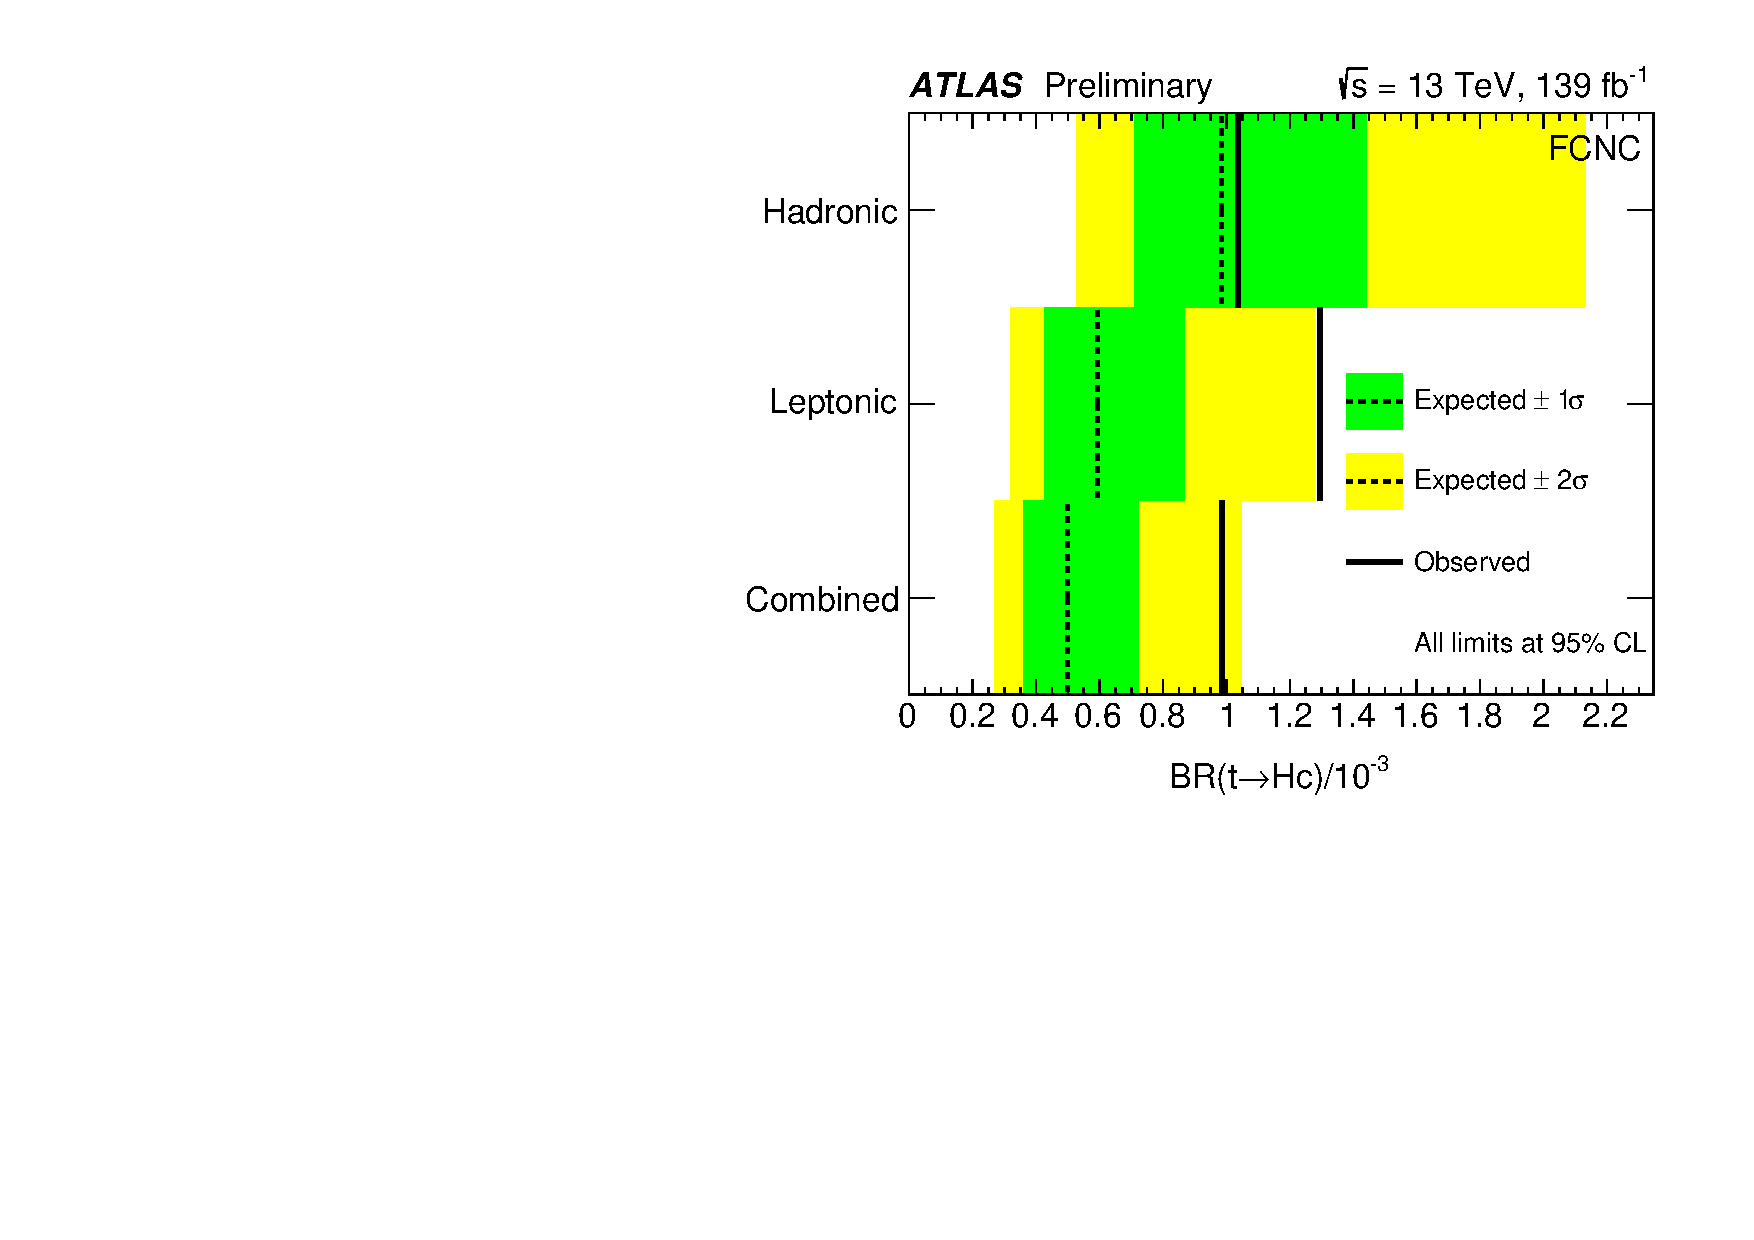
\includegraphics[width=0.49\textwidth]{figures/tcH_Limits.pdf}&
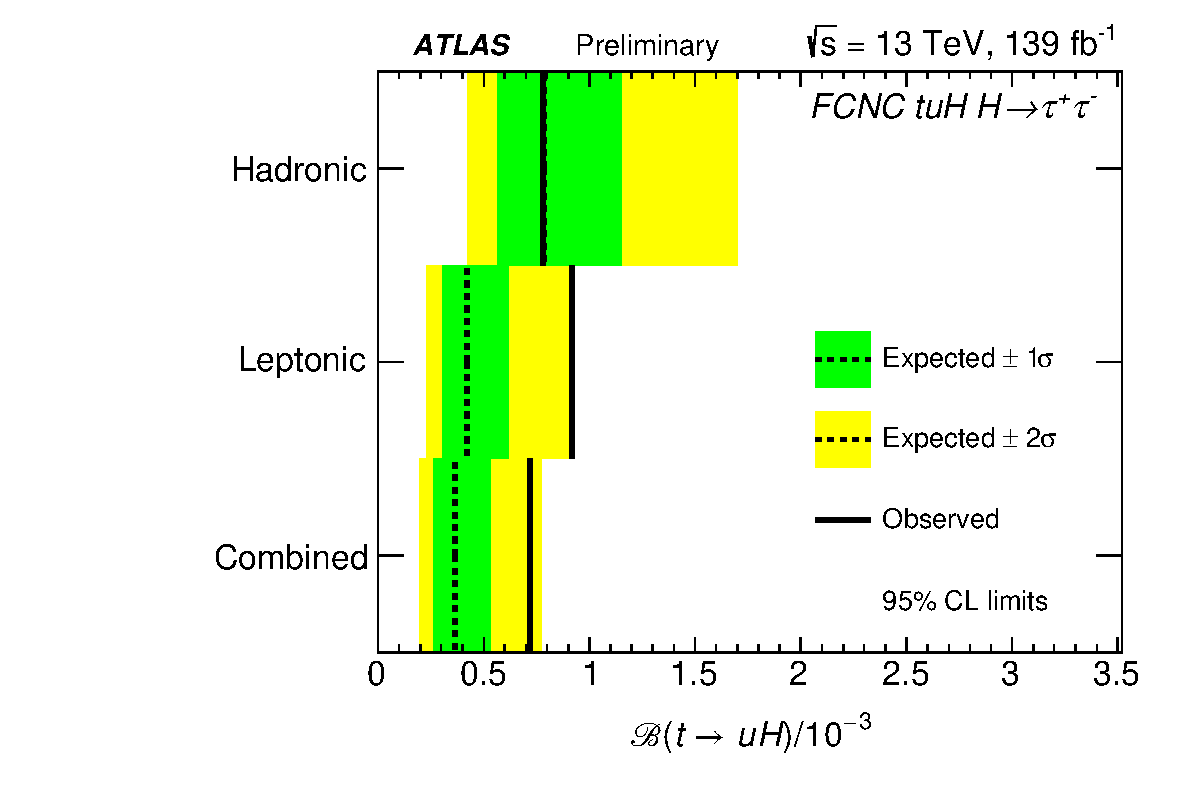
\includegraphics[width=0.49\textwidth]{figures/tuH_Limits.pdf}\\
(a) $tcH$ & (b) $tuH$ \\
\end{tabular}
\caption{\small {(a) This figure shows 95\% CL upper limits on $\BR(t\to cH)$ for the individual searches as well as their
combination, assuming $\BR(t\to uH)=0$. (b) This figure shows 95\% CL upper limits on $\BR(t\to uH)$ for the individual searches as well as their
combination, assuming $\BR(t\to cH)=0$. The observed limits (solid lines) are compared with the 
expected (median) limits under the background-only hypothesis (dotted lines). The surrounding shaded bands correspond to the 68\% and 95\% CL intervals around the expected limits, 
denoted by $\pm 1\sigma$ and $\pm 2\sigma$ respectively.
}}
\label{fig:limits_combo_1D_hc} 
\end{center}
\end{figure*}
%%%%%%%%%%%%%%

%%%%%%%%%%%%%%%%%%
%%%%\begin{figure*}[h!]
%%%%\begin{center}
%%%%\includegraphics[width=0.7\textwidth]{figures/tuH_combined_Limit.pdf}
%%%%\caption{\small {95\% CL upper limits on $\BR(t\to Hu)$ for the individual searches as well as their
%%%%combination, assuming $\BR(t\to Hc)=0$. The observed limits (solid lines) are compared with the 
%%%%expected (median) limits under the background-only
%%%%hypothesis (dotted lines). The surrounding shaded bands correspond to the 68\% and 95\% CL intervals around the expected limits, 
%%%%denoted by $\pm 1\sigma$ and $\pm 2\sigma$, respectively.
%%%%}}
%%%%\label{fig:limits_combo_1D_hu} 
%%%%\end{center}
%%%%\end{figure*}

A similar set of results can be obtained by simultaneously varying both branching ratios in the likelihood function.
Figure~\ref{fig:limits_combo_2D}(a) shows the 95\% CL upper limits on the branching ratios in the $\BR(t\to uH)$ versus $\BR(t\to cH)$ plane. 
%The small differences between the limiting values (on the $x$- and $y$-axes) of the branching ratio limits obtained in the two-dimensional scan and 
%those reported in Table~\ref{tab:limits_summary}, result from slightly different choices in the $\HML$ search  
%regarding the final discriminant, which in the two-dimensional case should be common to both signals, and its binning.
%\textbf{Add comment of what discriminant is used in this case and the caveat regarding the corresponding 1D limit.}
The corresponding upper limits on the D6 Wilson coefficient couplings in the $C_{u\phi}$ versus $C_{c\phi}$ plane are shown in Figure~\ref{fig:limits_combo_2D}(b).

\begin{figure*}[t!]
\begin{center}
\subfloat[]{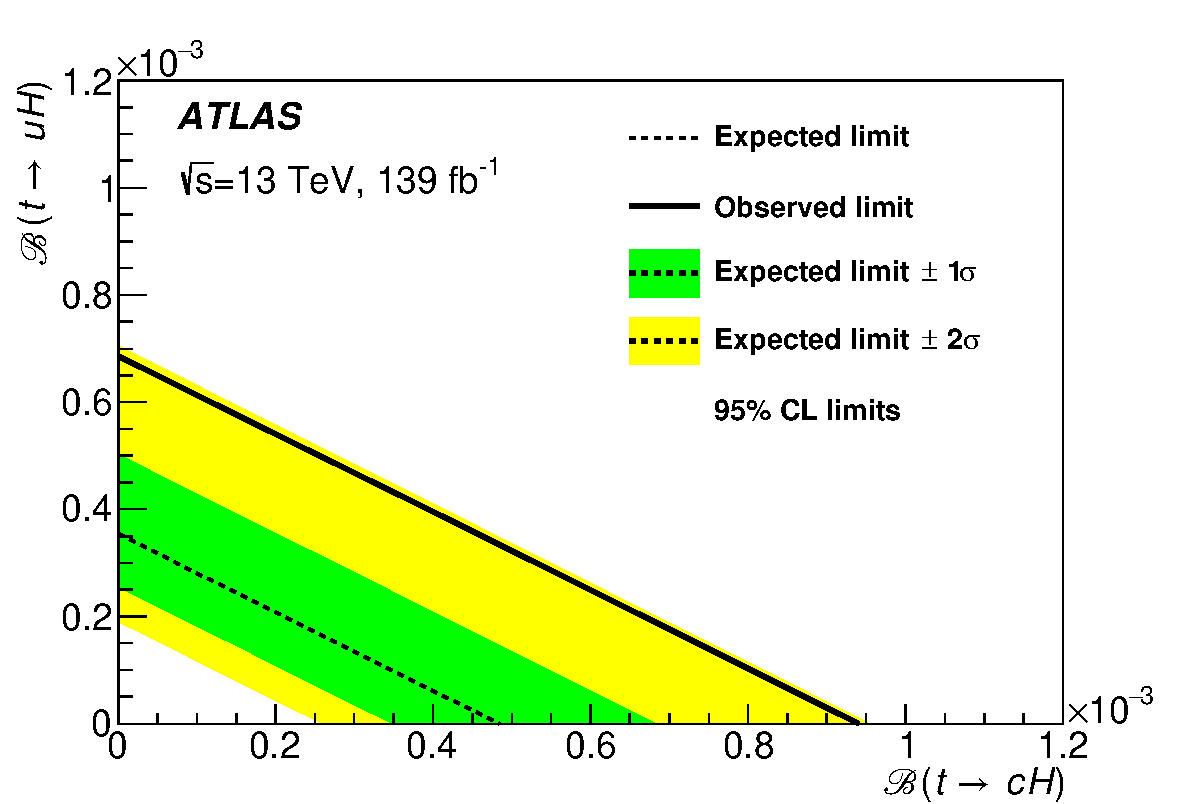
\includegraphics[width=0.49\textwidth]{figures/2DLimits.pdf}}
\subfloat[]{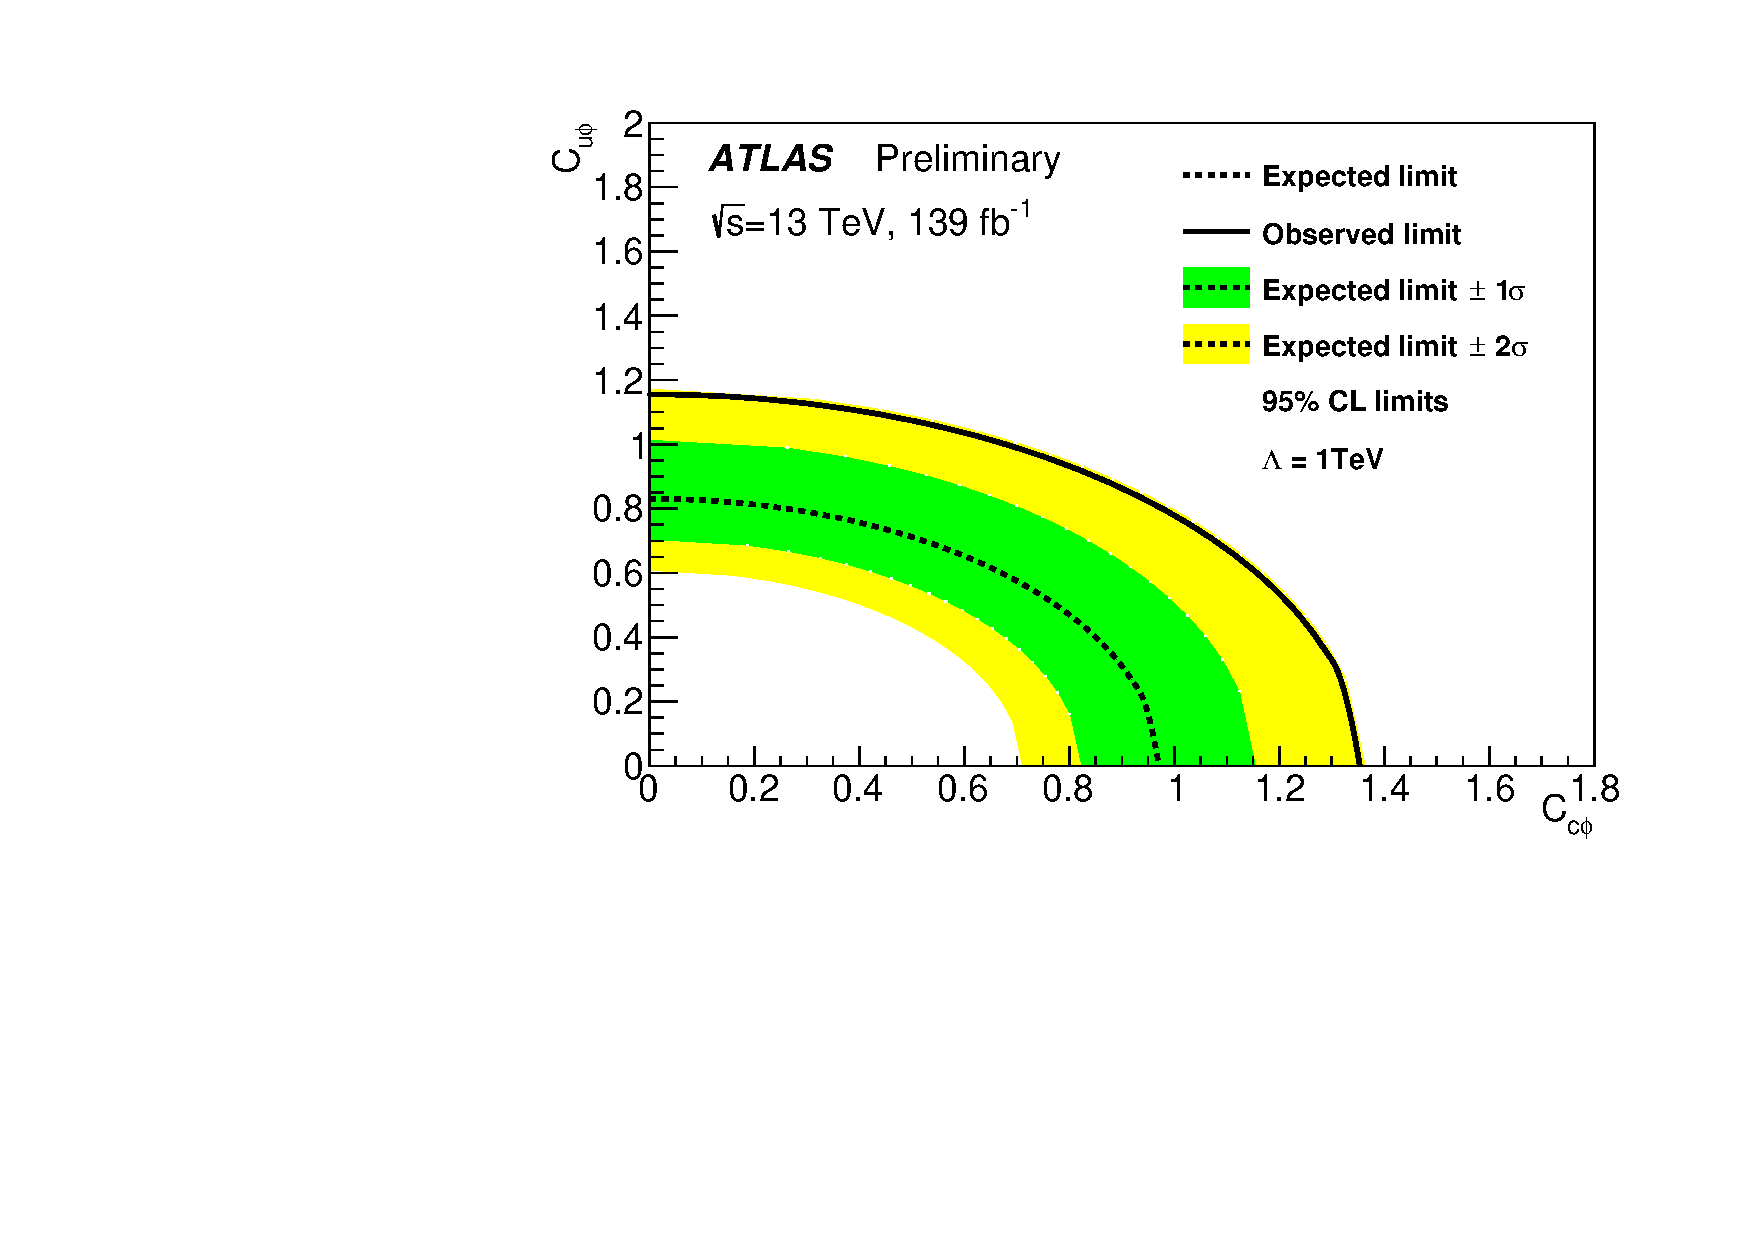
\includegraphics[width=0.49\textwidth]{figures/Wilson_coefficient_smooth.pdf}}
\caption{\small {95\% CL upper limits (a) in the $\BR(t\to cH)$ versus $\BR(t\to uH)$ plane and (b) in the 
$C_{c\phi}$ versus $C_{u\phi}$ plane for the combination of the searches. The observed limits (solid lines) are compared with the expected (median) limits under the background-only hypothesis (dotted lines). The surrounding shaded bands correspond to the 68\% and 95\% CL intervals around the expected limits, 
denoted by $\pm 1\sigma$ and $\pm 2\sigma$ respectively.}}
%%=======
%%of $C_{u\phi}$ versus $C_{c\phi}$ for the combination of the searches. The observed limits (solid lines) are compared with the expected (median) limits under the background-only hypothesis (dotted %%lines). The surrounding shaded bands correspond to the 68\% and 95\% CL intervals around the expected limits, 
%%denoted by $\pm 1\sigma$ and $\pm 2\sigma$, respectively. ({\color{red} plot (b) needs to be updated}) }}
%%>>>>>>> e84999e0023e50e93b4b7507152380195248366c
\label{fig:limits_combo_2D} 
\end{center}
\end{figure*}
%%%%%%%%%%%%%%





%\begin{table}
%\caption{ Summary of fake tau scale factors derived in ttCRs. The numbers are shown as: nominal values,statistical errors and systematics erros. }
%\begin{center}
%\begin{tabular}{lcccccc}
%\toprule\toprule
%
%\multirow{2}{*}{Fake Factor Types} & \multicolumn{3}{c}{1 prong}                                                        & \multicolumn{3}{c}{3 prong}  \\
%                                &  $25-35$ GeV  & $35-45$ GeV  &  $45-$ GeV                                             &  $25-35$ GeV  & $35-45$ GeV       &  $45-$ GeV  \\
%\midrule
%Type-1                          &$0.71 \pm 0.01 \pm 0.03 $ &$0.61 \pm 0.02 \pm 0.04 $ &$0.38 \pm 0.02 \pm 0.05 $        & $1.01 \pm 0.03 \pm 0.04 $ & $1.09 \pm 0.04 \pm 0.05 $ & $0.30 \pm 0.05 \pm 0.07 $ \\
%% W fake OS       
%Type-2                          &$0.76 \pm 0.06 \pm 0.04 $ & $0.37 \pm 0.08 \pm 0.02$ & $0.74 \pm 0.08 \pm 0.02 $       & $0.93 \pm 0.10 \pm 0.04 $ & $1.05 \pm 0.09 \pm 0.03 $ & $0.79 \pm 0.09 \pm 0.04 $ \\
%% W fake SS          
%Type-3                          &$0.62 \pm 0.10 \pm 0.03 $ &$0.83 \pm 0.09 \pm 0.03 $ &$0.94 \pm 0.07 \pm 0.02 $        & $1.07 \pm 0.13 \pm 0.03 $ &$1.39 \pm 0.12 \pm 0.03 $ &$1.26 \pm 0.10 \pm 0.04 $  \\
%%  b fake       
%Type-4                          &$1.20 \pm 0.02 \pm 0.01 $ & $1.01 \pm 0.04 \pm 0.02 $ &$0.76 \pm 0.03 \pm 0.03 $       &$1.28 \pm 0.07 \pm 0.02 $ &$0.66 \pm 0.08 \pm 0.01 $ & $0.71 \pm 0.07 \pm 0.02 $ \\
%% other fake
%\bottomrule\bottomrule
%\end{tabular}
%\label{tab:ff_summary}
%\end{center}
%\end{table}


%\begin{table}
%\caption{ Summary of fake tau (1-prong) scale factors derived in ttCRs. The numbers are shown as: nominal values,statistical errors and systematics erros. }
%\begin{center}
%\begin{tabular}{lcccccc}
%\toprule\toprule

%\multirow{2}{*}{Fake Factor Types} & \multicolumn{3}{c}{1 prong}  \\                                                
%                                   &  $25-35$ GeV  & $35-45$ GeV  &  $45-$ GeV            \\                           
%\midrule
%Type-1                          &$0.71 \pm 0.01 \pm 0.03 $ &$0.61 \pm 0.02 \pm 0.04 $ &$0.38 \pm 0.02 \pm 0.05 $  \\
%% W fake OS       
%Type-2                          &$0.76 \pm 0.06 \pm 0.04 $ & $0.37 \pm 0.08 \pm 0.02$ & $0.74 \pm 0.08 \pm 0.02 $ \\
%% W fake SS          
%Type-3                          &$0.62 \pm 0.10 \pm 0.03 $ &$0.83 \pm 0.09 \pm 0.03 $ &$0.94 \pm 0.07 \pm 0.02 $  \\
%%  b fake       
%Type-4                          &$1.20 \pm 0.02 \pm 0.01 $ & $1.01 \pm 0.04 \pm 0.02 $ &$0.76 \pm 0.03 \pm 0.03 $  \\
%% other fake
%\bottomrule\bottomrule
%\end{tabular}
%\label{tab:ff1_summary}
%\end{center}
%\end{table}


%\begin{table}
%\caption{ Summary of fake tau (3-prong) scale factors derived in ttCRs. The numbers are shown as: nominal values,statistical errors and systematics erros. }
%\begin{center}
%\begin{tabular}{lcccccc}
%\toprule\toprule

%\multirow{2}{*}{Fake Factor Types}        & \multicolumn{3}{c}{3 prong}  \\

%\begin{table}
%\caption{ Summary of fake tau (3-prong) scale factors derived in ttCRs. The numbers are shown as: nominal values,statistical errors and systematics erros. }
%\begin{center}
%\begin{tabular}{lcccccc}
%\toprule\toprule

%\multirow{2}{*}{Fake Factor Types}        & \multicolumn{3}{c}{3 prong}  \\
%                                          &  $25-35$ GeV  & $35-45$ GeV       &  $45-$ GeV  \\
%\midrule
%Type-1                                    & $1.01 \pm 0.03 \pm 0.04 $ & $1.09 \pm 0.04 \pm 0.05 $ & $0.30 \pm 0.05 \pm 0.07 $ \\
%% W fake OS
%Type-2                                    & $0.93 \pm 0.10 \pm 0.04 $ & $1.05 \pm 0.09 \pm 0.03 $ & $0.79 \pm 0.09 \pm 0.04 $ \\
%% W fake SS
%Type-3                                    & $1.07 \pm 0.13 \pm 0.03 $ &$1.39 \pm 0.12 \pm 0.03 $ &$1.26 \pm 0.10 \pm 0.04 $  \\
%%  b fake
%Type-4                                    &$1.28 \pm 0.07 \pm 0.02 $ &$0.66 \pm 0.08 \pm 0.01 $ & $0.71 \pm 0.07 \pm 0.02 $ \\
%% other fake
%\bottomrule\bottomrule
%\end{tabular}
%\label{tab:ff2_summary}
%\end{center}
%\end{table}


